\documentclass[12pt,a4paper,openright,twoside]{book}
\usepackage[utf8]{inputenc}
\usepackage{disi-thesis}
\usepackage{code-lstlistings}
\usepackage{notes}
\usepackage{shortcuts}
\usepackage{acronym}
\usepackage{rotating}
\usepackage[nobiblatex]{xurl}

\school{\unibo}
\programme{Corso di Laurea Magistrale in Ingegneria e Scienze Informatiche}
\title{Processo di Transizione e Reingegnerizzazione di un Pannello Web per DNS Filtering}
\author{Alberto Spadoni}
\date{\today}
\subject{Paradigmi di Programmazione e Sviluppo}
\supervisor{Prof. Mirko Viroli}
\cosupervisor{Dott. Nicolas Farabegoli}
\morecosupervisor{Dott. Gianluca Aguzzi}
\session{IV}
\academicyear{2023-2024}

% Definition of acronyms
\acrodef{IoT}{Internet of Thing}
\acrodef{vm}[VM]{Virtual Machine}

\mainlinespacing{1.241} % line spacing in mainmatter, comment to default (1)

\begin{document}

\frontmatter\frontispiece

\begin{abstract}
  Max 2000 characters, strict.
\end{abstract}

\begin{dedication} % this is optional
  Alla mia famiglia, a Lara
\end{dedication}

%----------------------------------------------------------------------------------------
\tableofcontents
\listoffigures
%----------------------------------------------------------------------------------------

\mainmatter

\chapter{Introduzione}

La presente tesi nasce dall’esperienza di tirocinio svolta presso un’azienda specializzata nello sviluppo di soluzioni per il filtraggio DNS. Durante tale esperienza, è stato possibile contribuire alle prime fasi di reingegnerizzazione del pannello Web per la configurazione di un filtro DNS. Questo pannello, concepito per offrire funzionalità di gestione e controllo dei domini da filtrare, presentava tuttavia limiti strutturali e tecnologici che ne ostacolavano la manutenibilità e l’estensibilità. L’esigenza di modernizzare l’architettura, migliorare l’esperienza utente e garantire maggiore sicurezza è nata anche dalla volontà di posizionare l’azienda in un mercato più orientato alle medie-grandi organizzazioni. Questo obiettivo mira a favorirne la crescita e a consolidarne il ruolo come punto di riferimento a livello globale nel settore del filtraggio DNS.

Il presente lavoro si inserisce in questo contesto, con l’obiettivo di progettare e sviluppare una nuova versione del pannello di configurazione del filtro DNS aziendale, adottando un’architettura moderna basata su microservizi. Questo approccio mira a garantire maggiore efficienza, sicurezza e manutenibilità rispetto alla versione precedente, superando le rigidità del legacy e introducendo nuove funzionalità essenziali.

Scopo dell’elaborato è fornire una visione organica del processo di reingegnerizzazione svolto, illustrando le motivazioni alla base della necessità di aggiornare il pannello, i principali obiettivi progettuali e i risultati raggiunti nelle prime fasi di sviluppo.

Il contesto teorico di riferimento comprende sia il Domain Name System (DNS), con le sue logiche di funzionamento e la sua importanza nella gestione del traffico in rete, sia le metodologie di reingegnerizzazione software, che offrono linee guida per affrontare in modo sistematico la modernizzazione di soluzioni esistenti.

Dal punto di vista metodologico, il progetto ha richiesto un'attenta fase di analisi, seguita dalla definizione di un’architettura più flessibile e scalabile, fino all’implementazione di un primo set di funzionalità.

Durante lo sviluppo, sono state affrontate diverse sfide, tra cui la transizione da un’architettura monolitica a una basata su microservizi, la riprogettazione della base dati e la creazione di un sistema avanzato di gestione degli errori, in grado di operare in modo strutturato e pervasivo su tutti i livelli del sistema.

\section{Struttura dell'elaborato}
L'elaborato è suddiviso nei seguenti capitoli, ciascuno dedicato a un aspetto specifico del progetto:

\begin{itemize}
  \item \textbf{Capitolo 2: Background} – Introduce il funzionamento del DNS e il filtraggio DNS, oltre alle metodologie di reingegnerizzazione software.
  \item \textbf{Capitolo 3: Analisi} – Esamina il sistema legacy, evidenziandone l’architettura, le tecnologie adottate e le limitazioni riscontrate. Inoltre, introduce i requisiti del nuovo sistema e la modellazione del dominio.
  \item \textbf{Capitolo 4: Design} – Presenta la nuova architettura proposta, sia lato frontend che backend, illustrando le interazioni tra i componenti e le principali scelte tecnologiche adottate.
  \item \textbf{Capitolo 5: Implementazione} – Descrive il processo di sviluppo del nuovo sistema, soffermandosi sull’infrastruttura, sull’organizzazione della repository e sull'implementazione del sistema di gestione degli errori.
  \item \textbf{Capitolo 6: Valutazione} – Analizza i requisiti soddisfatti e le funzionalità implementate, confrontandole con gli obiettivi iniziali. Inoltre, discute i miglioramenti pianificati e gli aspetti ancora da sviluppare.
  \item \textbf{Capitolo 7: Conclusione} – Riassume il lavoro svolto, evidenziando le principali lezioni apprese e proponendo possibili sviluppi futuri del sistema.
\end{itemize}

Grazie a questa suddivisione, l’elaborato mira a fornire una panoramica completa del percorso di reingegnerizzazione del sistema, dall’analisi dei requisiti iniziali fino alle valutazioni finali e ai suggerimenti per successivi sviluppi. L’obiettivo ultimo è offrire un contributo concreto alla modernizzazione del software, ponendo le basi per futuri interventi di mantenimento e potenziamento del sistema.

\chapter{Stato dell'Arte}

\section{Introduzione al DNS e al filtraggio}
Prima di trattare l'argomento cardine del presente capitolo, si ritiene opportuno fare una breve panoramica sui concetti importanti ad esso collegati. Verrà in prima batttuta presentato il Domain Name System (DNS), che può essere definito come uno dei pilastri fondamentali di tutta l'architettura della rete Internet. Successivamente, ci si sposterà sull'ambito del filtraggio in Internet, che rappresenta il contesto più ampio di cui il filtraggio DNS fa parte.

\subsection{Cos'è il DNS e il suo ruolo in Internet}
Il Domain Name System è un database gerarchico e distribuito che contiene le associazioni tra nomi di dominio ed altre importanti informazioni, tra cui gli indirizzi IP.

Questo fondamentale sistema consente agli utenti di localizzare le risorse sulla rete andando a convertire nomi di dominio familiari ed in formato leggibile dagli umani in indirizzi numerici ai quali un computer può connettersi. Un'analogia comune che si uutilizza per spiegare il ruolo dei sistema DNS è che esso serve da rubrica telefonica per Internet, andando a tradurre i nomi di computer comprensibili agli umani nei relativi indirizzi numerici interpretabili dalle macchine. Per fare un esempio, il nome di dominio \texttt{www.airbus.com} viene tradotto dal DNS nell'indirizzo IPv4 \texttt{107.154.76.155}.

\subsubsection{Vulnerabilità del DNS e necessità di filtraggio}
Il DNS rappresenta una porzione cruciale della rete Internet e per questo motivo la sua messa in sicurezza risulta molto importante. Infatti, se un individuo malintenzionato dovesse riuscire a comprometterlo, sarebbe in grado di bloccare, o comunque ridurre, le normali attività che avvengono sulla rete.

Il sistema in oggetto è stato progettato negli anni '80 per rispondere alla necessità di una risoluzione dei nomi rapida e scalabile su una rete in continua espansione. Al momento della sua concezione, come descritto nelle specifiche originarie RFC 1034 \cite{rfc1034} e RFC 1035 \cite{rfc1035}, l'attenzione era principalmente concentrata sulla funzionalità e sull'efficienza, senza considerare i potenziali problemi di sicurezza che sarebbero emersi con la crescita esponenziale di Internet. Oltretutto, la solida fiducia che le specifiche RFC trasmettevano ai professionisti IT dell’epoca non li spinse a preoccuparsi o a indagare sui potenziali rischi di sicurezza che tale sistema poteva comportare \cite{hudaib2014dns}. Questa scelta rifletteva il contesto storico in cui è nato il DNS: la rete era allora utilizzata principalmente da enti accademici e governativi, con un livello di fiducia reciproca tra i partecipanti. Tuttavia, con l'apertura di Internet a un pubblico globale, il DNS ha rivelato vulnerabilità intrinseche, tra cui la mancanza di meccanismi nativi che garantiscano l'autenticazione delle risposte e l'integrità delle informazioni da esso fornite. Tali lacune hanno reso possibile una serie di attacchi che sfruttano le debolezze proprie del sistema DNS. Tra questi, si annoverano il DNS Spoofing, gli attacchi di tipo Distributed Denial of Service (DDoS) nei confronti dell'infrastruttura DNS e il DNS Hijacking.

\paragraph{DNS Spoofing}
Il DNS spoofing, noto anche come Cache Poisoning, consiste nell'iniettare dati malevoli nella cache dei server DNS bersaglio, inducendoli a restituire informazioni errate agli utenti. Questo attacco permette ai malintenzionati di reindirizzare il traffico verso siti controllati da essi, facilitando il furto di credenziali o altre forme di attacchi avanzati. Un esempio storico di DNS spoofing è l'attacco di Eugene Kashpureff del 1997, il quale riuscì a reindirizzare tutti i visitatori del dominio \texttt{internic.net} verso il sito della compagnia Alternic, di cui era il fondatore \cite{lioy2000dns}. In generale, questa tipologia di attacco sfrutta la mancanza di autenticazione nelle risposte DNS e l'assenza di integrità nelle informazioni memorizzate nella cache. I metodi per mitigare il DNS spoofing includono sostanzialmente l'implementazione di DNSSEC, che garantisce l'autenticità delle risposte attraverso firme digitali \cite{rfc2535}.

\paragraph{Attacchi di amplificazione DNS}
Gli attacchi Distributed Denial of Service (DDoS) rappresentano una minaccia critica e persistente per la sicurezza informatica. In generale, essi mirano a compromettere la disponibilità dei servizi di un sistema bersaglio, costringendolo a un riavvio forzato o esaurendone le risorse, come cicli della CPU, memoria RAM o larghezza di banda di rete. A conseguenza di ciò, il sistema attaccato diventa incapace di fornire i servizi previsti agli utenti legittimi.

Tra le più comuni applicazioni del DDoS nei confronti dell'infrastruttura DNS è possibile trovare i cosiddetti DNS Amplification Attacks, in cui un attaccante invia richieste al Domain Name System con un indirizzo IP sorgente falsificato, facendole apparire come provenienti dalla vittima. A questo punto, i server DNS rispondono con pacchetti di dimensioni molto superiori rispetto alla richiesta iniziale, amplificando così il traffico diretto alla vittima.
%
Il principio alla base di questa tecnica risiede nella capacità degli attaccanti di sfruttare la differenza tra la dimensione delle richieste e quella delle risposte. Ad esempio, una richiesta per un grande file di zona DNS, con l'indirizzo IP sorgente falsificato, viene inviata a un numero significativo di server DNS pubblici. Questi, ignari della natura fraudolenta delle richieste, rispondono inviando i dati direttamente alla vittima designata. La differenza di dimensioni tra la richiesta, tipicamente piccola, e la risposta, significativamente più grande, permette agli attaccanti di moltiplicare il volume di traffico generato, compromettendo gravemente il sistema bersaglio \cite{Alieyan2016}.

Un esempio di amplificazione DNS è quello che ha colpito Spamhaus nel 2013, considerato uno dei più grandi attacchi DDoS mai accaduti. Esso è stato caratterizzato da una richiesta di 36 byte che ha generato una risposta di 3.000 byte, amplificando il traffico di un fattore 100 e generando un volume di dati in entrata ai server della compagnia pari a 75GBps \cite{Bonasera2021}.

\paragraph{DNS Hijacking}
Il DNS hijacking prevede la compromissione di server DNS o la manipolazione delle configurazioni DNS di un utente per reindirizzare il traffico verso destinazioni controllate dall'attaccante. Questo attacco può essere implementato attraverso malware che modifica le impostazioni DNS locali o mediante la compromissione diretta dei server DNS \cite{hudaib2014dns}.

Le conseguenze includono il furto di credenziali, la diffusione di malware e la censura di contenuti web. Alcuni provider di servizi Internet (ISP) utilizzano questa tecnica per scopi commerciali, come la visualizzazione di pubblicità. Per mitigare il DNS hijacking, si consiglia di utilizzare configurazioni DNS sicure, abilitare DNSSEC e controllare in maniera scrupolosa le modifiche ai record DNS \cite{hudaib2014dns}.

\paragraph{Necessità di un filtraggio DNS}
Per affrontare queste problematiche, il filtraggio DNS rappresenta una soluzione efficace e scalabile. Oltre a bloccare domini malevoli, consente di ottimizzare l'uso delle risorse di rete e garantire conformità normativa. Tuttavia, la sua implementazione richiede un bilanciamento tra sicurezza e accessibilità, minimizzando l'impatto sulle prestazioni.

\subsection{Il filtraggio Internet e il posizionamento del DNS filtering}

\chapter{Analisi}
Il presente capitolo fornisce un'analisi introduttiva sul sistema legacy, descrivendone le funzionalità principali, l'architettura e le tecnologie impiegate. Verranno evidenziati i limiti strutturali e operativi che hanno portato l'azienda a intraprendere un processo di reingegnerizzazione, con l'obiettivo di sviluppare un sistema più moderno, scalabile e manutenibile.

Un aspetto cruciale di questa analisi riguarda la strategia di transizione dal sistema legacy al nuovo pannello di configurazione. Inizialmente era stata prevista una coesistenza graduale tra i due sistemi, ma la direzione aziendale ha successivamente deciso di adottare un approccio differente. Il nuovo sistema verrà sviluppato fino a includere tutte le macrofunzionalità fondamentali, che gli garantiranno una quasi completa operatività. Inoltre, sarà introdotta una nuova funzionalità che, oltre a rappresentare un'evoluzione rispetto al legacy, contribuirà a differenziare il nuovo sistema e a valorizzarne le potenzialità.
%
Solo una volta completato, il nuovo pannello sostituirà integralmente il legacy con una transizione netta, eliminando quindi la necessità di retrocompatibilità e riducendo la complessità della fase transitoria.

Proseguendo, il capitolo illustrerà gli obiettivi e i requisiti principali che hanno guidato la progettazione del nuovo sistema, preparando la discussione del capitolo successivo, in cui verranno descritte nel dettaglio le scelte architetturali adottate per superare le limitazioni del sistema legacy e rispondere alle nuove esigenze aziendali e di mercato.

Infine, la parte finale del capitolo sarà dedicata all'analisi del dominio applicativo, con l'obiettivo di identificare i concetti e le entità fondamentali del sistema legacy che verranno utilizzati per la progettazione del nuovo sistema. Questa analisi è essenziale per definire una base strutturata su cui modellare le funzionalità del nuovo pannello di configurazione, garantendo una transizione coerente e ben organizzata dalle logiche del sistema precedente a quelle della nuova implementazione.

\section{Introduzione al sistema esistente}
Il sistema legacy qui esaminato rappresenta un pannello Web utilizzato dall'azienda \textit{FlashStart Group srl}\footnote{\url{https://flashstart.com}} per la gestione e la configurazione del suo filtro DNS. L’analisi in questione, effettuata nell’ambito di un tirocinio in preparazione della presente tesi, si basa sulle osservazioni dirette fatte durante lo sviluppo del nuovo sistema, dato che la documentazione del legacy risulta pressoché assente.

Come illustrato in \Cref{fig:flashstart-legacy}, il pannello legacy offre una dashboard che riporta statistiche sulle richieste DNS processate, suddivise tra richieste bloccate, consentite e non risolte, con grafici relativi alle categorie più filtrate e ai servizi più bloccati. L’interfaccia presenta un'organizzazione a schede, con una barra superiore per la selezione del cliente e dei profili associati.
%
Nonostante le funzionalità offerte, il design risulta datato e poco curato dal punto di vista estetico, con un layout che non trasmette immediatamente la professionalità del prodotto e non valorizza l’esperienza utente.

\begin{figure}
  \centering
  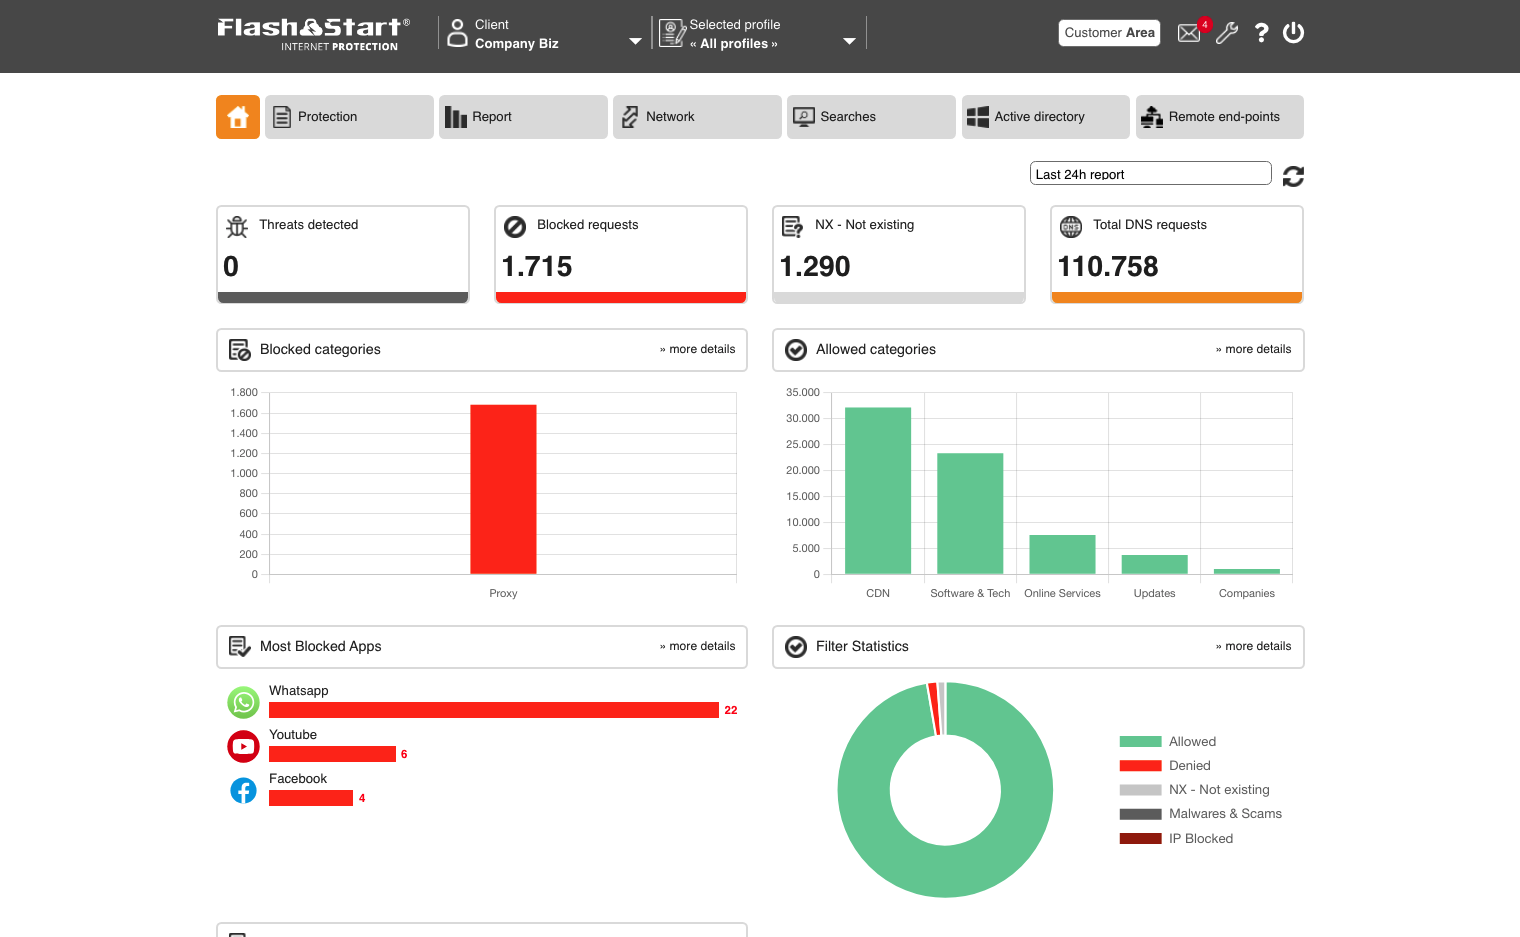
\includegraphics[width=1\textwidth]{figures/old-home.png}
  \caption{Schermata principale del pannello Web legacy di FlashStart.}
  \label{fig:flashstart-legacy}
\end{figure}

\subsubsection{Terminologia e definizioni}
Da qui in avanti verranno utilizzate alcune terminologie specifiche che descrivono concetti e funzionalità del sistema legacy. Pertanto, prima di proseguire con la sua analisi, è opportuno fornire una breve spiegazione di questi termini, utilizzati dall'azienda per rappresentare concetti chiave del dominio applicativo.

\begin{itemize}
  \item \textbf{Rete}: identifica un indirizzo IP registrato nel sistema e associato alla sede di un cliente, come ad esempio una scuola. Le reti possono essere statiche (IP pubblico fisso) o dinamiche (IP pubblico variabile).

  \item \textbf{Endpoint}: rappresenta un dispositivo fisico specifico registrato nel sistema, come un computer o uno smartphone. A differenza della rete, un endpoint è associato direttamente a un dispositivo, piuttosto che a un indirizzo IP generico.

  \item \textbf{Dealer}: un rivenditore che vende licenze del filtro DNS ai clienti finali, i quali devono, in autonomia, configurare le proprie policy di sicurezza tramite il pannello Web.

  \item \textbf{Managed Service Provider (MSP)}: è un particolare tipo di Dealer che, oltre a vendere licenze, si occupa anche della configurazione e della gestione delle policy di sicurezza per i propri clienti. A differenza dei precedenti fornitori di servizi, gli MSP impediscono ai clienti finali di accedere al pannello, occupandosi interamente della gestione.

  \item \textbf{Whitelabel}: una funzionalità che consente ai fornitori di servizi, come i Dealer, di personalizzare il pannello Web con il proprio logo, colori e branding, nascondendo ogni riferimento al produttore originale del sistema.

  \item \textbf{ClientShield}: è un'applicazione per computer e dispositivi mobili sviluppata dall'azienda, che consente di registrare un endpoint nel sistema e sfruttare il filtro DNS anche al di fuori della rete usuale.
\end{itemize}

\subsection{Panoramica sulle funzionalità}
Il pannello Web legacy rappresenta lo strumento principale per la gestione e configurazione del filtro DNS offerto dall'azienda. Nonostante le limitazioni architetturali e tecnologiche, il sistema fornisce un insieme di funzionalità che consentono agli utenti di configurare, monitorare e amministrare le policy di filtraggio DNS. Di seguito viene fornita una panoramica delle principali funzionalità offerte dal suddetto pannello.

\subsubsection{Gestione delle policy di protezione}
Il pannello consente di creare e configurare diversi profili di protezione, ciascuno dei quali può includere una combinazione personalizzata di filtri per:
\begin{itemize}
  \item Bloccare minacce informatiche come malware e phishing;
  \item Limitare l'accesso a contenuti specifici, come siti per adulti o contenuti inappropriati;
  \item Bloccare l'accesso ad applicazioni o servizi specifici, divisi per categoria di appartenenza;
  \item Bloccare l'accesso a pagine Web e servizi provenienti da determinate aree geografiche.
\end{itemize}

Per aumentare il grado di flessibilità del filtro, gli utenti possono creare delle liste di accesso personalizzate, tra cui:
\begin{itemize}
  \item \textbf{Allow list}: per consentire l'accesso a domini specifici;
  \item \textbf{Block list}: per bloccare domini o indirizzi IP specifici.
\end{itemize}
Queste liste possiedono una priorità più elevata rispetto alle funzioni di protezione citate in precedenza. Per questo motivo, esse consentono di specificare delle \emph{eccezioni} rispetto alle normali policy di sicurezza. Ad esempio, è possibile concedere l'accesso ad un contenuto di norma non consentito, oppure bloccare un dominio che risulta legittimo.

\subsubsection{Gestione delle reti di protezione}
Un'altra funzionalità fondamentale del pannello è la possibilità di specificare quali reti devono essere sottoposte al filtraggio, garantendo un controllo preciso e mirato sulle attività DNS. Questo permette di configurare reti aziendali o domestiche in modo che tutte le richieste DNS generate da tali indirizzi IP passino attraverso le policy di protezione impostate. La configurazione delle reti di protezione può essere adattata a diverse esigenze, supportando due principali modalità:
\begin{itemize}
  \item \textbf{IP pubblico statico}: questa configurazione è utilizzata quando la rete dispone di un IP pubblico statico, ovvero un indirizzo IP assegnato in modo permanente dal proprio ISP. In questo caso, il pannello consente di associare le policy di filtraggio a una rete identificata da uno specifico IP, garantendo che tutte le richieste DNS provenienti da tale rete siano sottoposte ai controlli e ai filtri impostati;

  \item \textbf{IP pubblico dinamico}: per le reti che non dispongono di un IP pubblico statico, il sistema supporta la configurazione tramite DynamicDNS\footnote{\url{https://www.rfc-editor.org/rfc/rfc2136.html}} (DDNS). Questo approccio consente di monitorare e filtrare le richieste DNS anche quando l’indirizzo IP della rete varia nel tempo, utilizzando un sistema di aggiornamento dinamico che associa un nome di dominio all’IP corrente della rete. Questo garantisce continuità nella protezione senza la necessità di aggiornamenti manuali.
\end{itemize}

\subsubsection{Visualizzazione e analisi dei report}
Il pannello offre una sezione dedicata alla generazione e analisi dei report relativi al traffico DNS della rete, permettendo di monitorare l’efficacia delle policy di filtraggio e di ottenere informazioni dettagliate sull’attività di rete in un determinato intervallo di tempo. Questi report forniscono una visione chiara e organizzata del comportamento della rete, aiutando gli utenti a identificare potenziali minacce e a ottimizzare le configurazioni esistenti.

\paragraph{Tipologie di report disponibili}
Tramite un menu a cascata, è possibile selezionare diversi tipi di report, tra cui:
\begin{itemize}
  \item \textbf{Bloccati per categoria}: mostrano le richieste DNS bloccate verso siti indesiderati, raggruppandole per categoria o macro-categoria;
  \item \textbf{Consentiti per paese o categoria}: forniscono il numero di richieste consentite, organizzate per paese o per categoria di contenuti;
  \item \textbf{Malware e minacce bloccate}: presentano un’analisi delle richieste che hanno attivato il filtro, indicando malware o altre minacce bloccate;
  \item \textbf{Traffico per fasce orarie o giorni}: permettono di analizzare le richieste DNS effettuate in specifiche fasce orarie o giorni della settimana;
  \item \textbf{Report geografici}: forniscono una mappa del mondo che evidenzia il traffico DNS suddiviso per paesi e continenti.
\end{itemize}

Dopo aver configurato i parametri di analisi, gli utenti possono generare i report secondo diverse modalità. Essi possono essere esportati in formato PDF, oppure inviati direttamente via e-mail a destinatari predefiniti. Inoltre, il pannello offre una funzione di pianificazione che consente di programmare l'invio automatico dei report a intervalli regolari, ad esempio su base settimanale, rendendo più efficiente il monitoraggio continuo.

\subsubsection{Gestione dei dispositivi protetti (Endpoint)}
Il pannello include anche una funzionalità per gestire i dispositivi su cui è installato il ClientShield. In particolare, questa configurazione permette di tracciare con precisione quale dispositivo ha originato una determinata richiesta DNS, fornendo un maggiore controllo e un livello di dettaglio maggiore sulle attività della rete.

\subsubsection{Funzionalità aggiuntive}
Oltre alle funzionalità principali già descritte, il pannello Web offre una serie di strumenti utili per migliorare la gestione e il controllo delle configurazioni. Tra queste, vi è la possibilità di personalizzare la pagina di blocco che viene visualizzata dagli utenti ogni volta che tentano di accedere a un dominio non consentito.
%
Il pannello consente anche di verificare facilmente a quale categoria appartiene un determinato sito Web, aiutando gli utenti a valutare come configurare al meglio le politiche di filtraggio.
%
Un’altra funzionalità interessante è la visualizzazione del traffico DNS in tempo reale, che fornisce un monitoraggio immediato dell’attività di rete. Inoltre, il sistema supporta l'importazione di domini in formato batch, permettendo di aggiungere rapidamente liste di siti Web consentiti o bloccati attraverso file di testo.

Per concludere la panoramica sulle funzionalità, il pannello possiede un'importante integrazione con la tecnologia Active Directory di Microsoft, che consente di ottenere informazioni dettagliate non solo sul dispositivo che ha originato una determinata richiesta DNS, ma anche sull’utente utilizzato per accedere a tale macchina.

\subsection{Architettura e tecnologie utilizzate}
Il pannello Web in esame, fino ad ora descritto solo dal punto di vista delle funzionalità, presenta un'architettura monolitica, tipica dei vecchi sistemi Web-based. Nonostante sia possibile identificare due macro-sezioni, denominate \textit{Customer area} e \textit{Pannello cloud}, non vi è una reale modularizzazione del frontend e del backend. Tutto il codice risulta scritto in modo procedurale, senza l’adozione di un paradigma orientato agli oggetti, e con una scarsa separazione delle responsabilità.

\subsubsection{Tecnologie utilizzate}
Il backend è interamente sviluppato in PHP, utilizzando un approccio ``plain'', ossia privo di framework moderni come Laravel\footnote{\url{https://laravel.com}}. Per il frontend sono stati utilizzati HTML, CSS e una versione obsoleta di jQuery\footnote{\url{https://jquery.com}} (\texttt{1.x}), che limita le possibilità di modernizzazione dell'interfaccia. In alcuni casi, il codice PHP si occupa anche di generare dinamicamente script JavaScript, i quali eseguono ulteriori chiamate a codice PHP lato server.

\subsubsection{Integrazione con API esterne}
L'azienda ha sviluppato un set di API pubbliche che consentono di gestire il filtro DNS senza dover necessariamente utilizzare il pannello Web in questione. Queste API offrono agli utenti la possibilità di integrare il filtro DNS in applicazioni personalizzate o di sviluppare un proprio client per la gestione delle configurazioni.

Nel tempo, alcune operazioni che il sistema legacy eseguiva direttamente sono state trasferite alle suddette API, le quali centralizzano la logica di business e gestiscono l'interazione con il database. Il pannello Web, in questi casi, funge da semplice interfaccia per chiamare le API. Tuttavia, molte operazioni continuano a risiedere direttamente sul sistema, implementando la logica applicativa e accedendo alla base dati.

\subsubsection{Gestione del database}
Il sistema legacy utilizza due database distinti per gestire le sue funzionalità e garantire la persistenza delle configurazioni. Entrambi adottano un motore di database \emph{relazionale}, che organizza i dati in tabelle collegate tra loro tramite un sistema di chiavi. La differenza principale risiede nella tecnologia sottostante: una base dati utilizza MySQL\footnote{\url{https://www.mysql.com}}, mentre l’altra è basata su PostgreSQL\footnote{\url{https://www.postgresql.org}}. Ciascuna di esse è destinata a scopi specifici e presenta caratteristiche diverse in termini di configurazione e prestazioni.

Il database MySQL è dedicato esclusivamente alla gestione delle licenze e dei dati anagrafici dei clienti. Esso viene ospitato su un server interno all’azienda e non è replicato in altre regioni. Questa configurazione rappresenta un collo di bottiglia significativo per gli utenti che sono distanti dalla sede aziendale, poiché tutte le richieste relative ai dati dei clienti o delle licenze (usate soprattutto nella fase di accesso al pannello) devono necessariamente essere inviate al server centrale per essere elaborate, causando latenze elevate.

Il database PostgreSQL, invece, è utilizzato per tutti gli altri dati, inclusi i report, le regole di protezione e le liste dei domini da bloccare. Questo database è configurato in replica globale, garantendo così prestazioni più elevate e tempi di risposta migliori per i clienti situati in diverse aree geografiche. Grazie a questa configurazione, i dati necessari al funzionamento del filtro DNS possono essere accessibili rapidamente da qualunque parte del mondo.

Un aspetto di fondamentale importanza per l'azienda è rappresentato dal contenuto del suddetto database, che costituisce un valore strategico significativo. Al suo interno, infatti, è presente una lista dei domini associati alla relativa categoria di appartenenza. Questa categorizzazione è utilizzata direttamente dal filtro DNS per bloccare l'accesso a determinati siti in base alle regole configurate dagli utenti. L'operazione di categorizzazione viene gestita internamente all'azienda e si basa su un approccio di intelligenza artificiale. Tale sistema analizza i testi delle pagine Web e determina automaticamente la categoria di appartenenza di ciascun dominio, migliorando l'efficacia del filtro DNS e arricchendo continuamente il patrimonio informativo dell'azienda.

\subsection{Limitazioni riscontrate}
Il sistema legacy presenta numerose limitazioni che hanno reso necessaria una completa reingegnerizzazione. Queste riguardano sia l’assenza di funzionalità fondamentali, come il supporto alla multiutenza, sia problematiche strutturali e di usabilità che compromettono la flessibilità e l’efficienza operativa dello stesso.

\subsubsection{Mancanza del supporto alla multiutenza}
Una delle principali limitazioni del sistema legacy, e tra quelle più sentite dai clienti dell'azienda, è l’assenza di un supporto per la multiutenza. Attualmente, infatti, il sistema permette a ciascun cliente di disporre di un unico account per accedere al pannello di configurazione, che possiede i privilegi di amministratore.

Questa mancanza rappresenta un ostacolo significativo, soprattutto per i dealer o gli MSP che integrano il filtro DNS in altri prodotti o lo rivendono ad aziende terze. Questi ultimi si trovano spesso a dover gestire configurazioni e politiche di protezione per conto dei loro clienti, ma l'assenza di un sistema multiutente impedisce di delegare determinate operazioni o di offrire accesso limitato a figure specifiche all’interno delle organizzazioni servite. Allo stesso modo, chi utilizza direttamente il pannello non può creare profili con permessi ridotti, ad esempio per utenti che necessitano soltanto di monitorare le configurazioni o consultare i report senza possibilità di modificarli.

Implementare la funzionalità in questione nel sistema attuale richiederebbe modifiche strutturali profonde, che non sono realisticamente attuabili senza un suo completo stravolgimento.

\subsubsection{Profili di protezione non condivisibili}
Un’altra significativa limitazione del sistema legacy riguarda l’impossibilità di condividere i profili di protezione tra diversi utenti. Attualmente, ogni profilo è strettamente associato a un singolo cliente, senza alcuna possibilità di essere condiviso o ereditato da altri. Questa carenza rappresenta un ostacolo rilevante, specialmente per gli MSP che gestiscono clienti con esigenze simili, come un gruppo di scuole o aziende dello stesso settore. In tali casi, sarebbe estremamente utile disporre di profili condivisi che consentano di applicare la stessa configurazione a più clienti contemporaneamente.
%
Inoltre, la mancanza di questa funzionalità aumenta il carico di lavoro in caso di modifiche alle regole di protezione. La situazione attuale, infatti, è tale per cui ogni variazione deve essere riportata manualmente su ciascun cliente, imponendo un processo lungo e soggetto a errori.

\subsubsection{Limiti e debolezze architetturali}
Il sistema legacy presenta numerosi limiti dovuti a scelte architetturali e tecnologiche datate, che influiscono negativamente sulla manutenibilità e sull'evoluzione del software. La mancanza di una chiara separazione tra frontend e backend complica la gestione del codice, rendendo difficoltosa l’adozione di nuove tecnologie. Oltretutto, pratiche quali l’utilizzo di PHP per generare dinamicamente codice JavaScript introducono ulteriore complessità ed opacità dei sorgenti, limitando la modularità e aumentando il rischio di commettere errori.

L’architettura monolitica rappresenta una delle principali debolezze del sistema. Qualsiasi modifica, anche minima, comporta interventi che possono avere ripercussioni su altre parti del codice, a causa dell’assenza di un design accurato e di una netta separazione delle responsabilità. Questo approccio non solo rallenta il ciclo di sviluppo, ma aumenta significativamente il rischio di regressioni e rende difficoltoso il debugging. La mancanza di modularità aggrava ulteriormente il problema: ogni nuova funzionalità o aggiornamento richiede un lavoro complesso e rischioso, che spesso si traduce in un incremento della fragilità del sistema.

\subsubsection{Problemi di usabilità}
L'interfaccia utente del sistema, sviluppata con tecnologie ormai obsolete, presenta diverse limitazioni che compromettono l’esperienza degli utenti finali. L’utilizzo di una versione datata di jQuery, unito all’assenza di un layout moderno, rende l’interfaccia poco intuitiva e difficile da navigare. Questi problemi non solo riducono l’efficienza operativa degli utenti, ma influenzano negativamente anche la percezione complessiva del sistema.

Un design grafico superato e poco efficiente limita, inoltre, la capacità del sistema di competere con soluzioni contemporanee, riducendone l’attrattiva sia per gli utenti attuali che per potenziali nuovi clienti.

\subsubsection{Conclusioni}
Le limitazioni evidenziate, che includono l’assenza di funzionalità essenziali come la multiutenza e i profili condivisibili, le debolezze architetturali e i problemi legati all’usabilità e all’interfaccia utente, mettono in luce la rigidità e l'obsolescenza del sistema legacy. Tali carenze ostacolano non solo l'efficienza operativa e la scalabilità del sistema, ma anche la capacità dell'azienda di rispondere alle richieste di mercato e di competere con soluzioni moderne. Questi fattori rendono indispensabile una completa reingegnerizzazione per soddisfare le esigenze attuali e future, garantendo al contempo un sistema moderno, scalabile ed efficiente.

\section{Esigenza di transizione tra i due sistemi}\label{sec:transizione}
La transizione dal sistema legacy al nuovo pannello di configurazione seguirà una strategia differente rispetto a quanto inizialmente previsto. Non sarà più adottato un approccio di coesistenza graduale tra i due sistemi, bensì una transizione netta non appena il nuovo sistema sarà pronto per il rilascio. Durante la fase di sviluppo, il vecchio pannello rimarrà l’unico utilizzato dagli utenti, mentre il nuovo verrà completato fino a includere tutte le macrofunzionalità fondamentali necessarie per garantirne l’operatività, oltre a una nuova funzionalità dedicata alla gestione dei profili condivisi. Solo a quel punto avverrà il passaggio definitivo al nuovo sistema.

Poiché gli utenti si ritroveranno i propri dati direttamente nel nuovo pannello, la migrazione delle informazioni dal legacy al nuovo sistema diventa un requisito fondamentale. Questo processo avverrà internamente all’azienda e dovrà garantire che tutti i dati necessari alle funzionalità trasferite siano disponibili nel nuovo sistema prima del rilascio. Le strategie di migrazione adottate dovranno assicurare la completa integrità e coerenza delle informazioni, evitando perdite o incongruenze tra i due ambienti.

Dopo il rilascio, la fase di transizione sarà limitata esclusivamente al periodo necessario per completare il trasferimento delle funzionalità minori ancora rimaste nel legacy. Tuttavia, rispetto all'approccio iniziale, non sarà più richiesta alcuna retrocompatibilità tra i due sistemi. Infatti, le funzionalità che continueranno a essere utilizzate nel legacy fino alla loro migrazione definitiva, non dovranno interagire con il nuovo sistema, evitando così complessità aggiuntive nella gestione dei dati.

Questa strategia di transizione consente di semplificare il passaggio al nuovo sistema, evitando la necessità di mantenere attivi entrambi i pannelli per un lungo periodo. Inoltre, riduce i rischi legati alla gestione della retrocompatibilità e permette di concentrare gli sforzi sullo sviluppo del nuovo sistema, senza vincoli imposti dall’integrazione con il legacy.

\section{Analisi del nuovo sistema}
\subsection{Obiettivi}
Il nuovo sistema nasce con l'obiettivo di posizionarsi come una soluzione moderna e professionale, capace di soddisfare le esigenze di un mercato in espansione e di attirare anche clienti di grandi dimensioni. Per raggiungere questo scopo è fondamentale che il pannello abbia un'interfaccia più curata e in linea con gli standard richiesti da organizzazioni complesse. Questo aspetto si inserisce in un più ampio percorso di rinnovamento della \textit{brand identity} aziendale, che include un nuovo logo, una palette di colori aggiornata e uno stile comunicativo uniforme.

Dal punto di vista tecnico, il sistema dovrà superare le limitazioni strutturali del legacy, modernizzando l'architettura per renderla più robusta e scalabile, in modo da poter gestire un numero crescente di utenti. Una delle priorità è quella di ridurre i tempi necessari per la manutenzione e l’aggiornamento, facilitando al contempo l’integrazione di nuove funzionalità.

Un obiettivo chiave della prima release del pannello è l'introduzione di funzionalità avanzate pensate per i fornitori di servizi, con particolare attenzione ai dealer e agli MSP. Tra queste, un ruolo centrale è ricoperto dai profili condivisi, noti anche come \textit{template}, che consentono di definire e applicare regole di protezione comuni a più clienti. Grazie ad i template, gli MSP potranno gestire in modo più efficiente le configurazioni, evitando di doverle replicare manualmente per ciascun cliente e permettendo la propagazione automatica delle modifiche.
%
Un'altra caratteristica fondamentale che differenzia questa prima versione da quella legacy è la presenza di una dashboard dedicata ai fornitori di servizi gestiti. Questo strumento consentirà loro di gestire in maniera completa ed efficace i clienti sotto la loro supervisione, offrendo una panoramica dettagliata sul traffico, sulle configurazioni applicate e sugli eventi di sicurezza rilevati. La dashboard sarà progettata per agevolare l’amministrazione su larga scala, semplificando operazioni come la modifica delle policy di protezione, l'assegnazione dei template e il monitoraggio centralizzato delle reti gestite.

Infine, una funzionalità fondamentale che differenzia questa prima versione da quella legacy è la gestione avanzata della multiutenza, una caratteristica assente nel sistema precedente. Nel nuovo pannello, sarà possibile associare più utenti a un singolo cliente, ciascuno con ruoli e permessi differenziati. Questo rappresenta un miglioramento significativo rispetto al passato, in cui l’accesso al pannello di configurazione era ristretto a un unico account per cliente. Grazie a questa funzione, più operatori all'interno di un'organizzazione potranno collaborare alla gestione delle policy di filtraggio DNS, con livelli di accesso che vanno dall'amministrazione completa alla sola consultazione dei report.

\subsection{Requisiti}
I requisiti riportati di seguito forniscono una panoramica delle funzionalità previste per il nuovo sistema. Tuttavia, solo una parte di essi è stata sviluppata o analizzata direttamente nel contesto del tirocinio in preparazione della presente tesi. Le funzionalità che verranno introdotte successivamente, pur essendo parte integrante del sistema finale, sono incluse in questa sezione per offrire una visione completa, ma non saranno trattate nel dettaglio in questo elaborato.

\subsubsection{Requisiti funzionali}
\begin{itemize}
  \item \textbf{Operatività del nuovo sistema al rilascio:}
    \begin{itemize}
      \item Il nuovo sistema deve includere fin dalla prima release tutte le macrofunzionalità necessarie per garantire la piena operatività del pannello di configurazione, in modo da consentire la transizione completa dal sistema legacy.
      \item Le funzionalità essenziali devono comprendere la gestione delle reti, la gestione utenti e permessi (compresa la multiutenza), la configurazione delle policy di filtraggio e la reportistica avanzata.
      \item Oltre a queste caratteristiche ereditate dal legacy, il nuovo sistema dovrà introdurre almeno una caratteristica distintiva rispetto alla versione precedente. In particolare, sarà implementata la gestione avanzata dei template, che consentirà di definire profili condivisi per applicare configurazioni comuni a più clienti.
      \item Prima della dismissione del sistema legacy, tutte le funzionalità previste dovranno essere completamente operative e testate su quello nuovo.
    \end{itemize}

  \item \textbf{Migrazione interna dei dati:}
    \begin{itemize}
      \item Tutti i dati del sistema legacy devono essere migrati nel nuovo sistema prima del rilascio, garantendo continuità operativa per gli utenti.
      \item Il processo di migrazione deve avvenire internamente all’azienda, senza richiedere interventi manuali da parte degli utenti finali.
      \item L’integrità e la coerenza dei dati devono essere assicurate, evitando perdite o incongruenze tra il vecchio e il nuovo sistema.
    \end{itemize}

  \item \textbf{Multiutenza e gestione utenti:}
    \begin{itemize}
      \item Il sistema deve supportare la multiutenza con ruoli differenziati, quali SuperAdmin, Admin e altri con permessi limitati.
      \item La creazione e la gestione degli utenti deve essere riservata agli amministratori.
    \end{itemize}

  \item \textbf{Dashboard per MSP:}
    \begin{itemize}
      \item Deve essere presente una schermata dedicata agli MSP, che fornisce loro una panoramica dei clienti gestiti.
      \item Tale panoramica deve includere report e statistiche aggregate che consentano di monitorare il traffico sulla rete e avere una visione completa sull'utilizzo del filtro.
      \item Deve inoltre essere presente la possibilità di impersonare uno dei clienti in gestione al fornitore di servizi, visualizzando il pannello come se tale cliente avesse effettuato l'accesso con il proprio account utente. L’MSP deve essere in grado non solo di visionare i report e le statistiche relative al cliente, ma anche di monitorare ed eventualmente modificare la sua configurazione del filtro.
      \item La schermata deve adattarsi dinamicamente in base al tipo di utente (MSP o cliente finale), mostrando solo i componenti grafici e le funzionalità a cui l’utente ha accesso.
    \end{itemize}

  \item \textbf{Gestione dei template di protezione:}
    \begin{itemize}
      \item Il sistema deve consentire la creazione e la gestione di template, che possono essere assegnati a diversi clienti.
      \item I template devono supportare opzioni di configurazione come categorie e applicazioni da bloccare, paesi da bloccare, attivazione SafeSearch e blocco completo tranne alcuni domini specifici.
      \item Le modifiche apportate ai template devono essere propagate automaticamente a tutti i clienti a cui sono stati assegnati.
      \item Devono essere disponibili template di eccezioni personalizzati, configurabili per soddisfare esigenze specifiche.
      \item Le liste di eccezioni devono poter essere importate nel sistema anche tramite file di testo in formato \texttt{.txt} o \texttt{.csv}.
    \end{itemize}

  \item \textbf{Reportistica:}
    \begin{itemize}
      \item Il sistema deve permettere di creare, visualizzare ed esportare report personalizzati.
      \item I report devono poter coprire intervalli temporali più estesi rispetto al legacy, passando da un mese a 3, 6 o anche 12 mesi per singolo report.
      \item Deve essere possibile pianificare l’invio automatico dei report via email, con frequenza settimanale o mensile.
    \end{itemize}
    \newpage
  \item \textbf{API pubbliche:}
    \begin{itemize}
      \item Il sistema deve offrire un set di API pubbliche per la gestione delle configurazioni, consentendo agli utenti di integrare il filtro DNS in applicazioni personalizzate o di sviluppare un proprio client per la gestione delle configurazioni.
      \item Le API devono supportare tutte le funzionalità disponibili tramite il pannello Web, inclusa la nuova gestione dei template.
      \item Le API devono essere provviste di una documentazione chiara e completa, che descriva i metodi disponibili e i relativi parametri.
    \end{itemize}

  \item \textbf{Notifiche:}
    \begin{itemize}
      \item Il sistema deve fornire notifiche direttamente nel pannello Web e via email.
      \item Le notifiche devono riguardare nuove funzionalità rilasciate, errori di rete e malware rilevati.
      \item Le notifiche via email devono includere report pianificati dagli utenti.
    \end{itemize}

  \item \textbf{Personalizzazione Whitelabel:}
    \begin{itemize}
      \item Il sistema deve supportare la personalizzazione whitelabel riservata ai Dealer, consentendo di modificare elementi come: nome, logo, palette di colori, menu, messaggi personalizzati al login, email per il supporto, notifiche e redirect.
    \end{itemize}

  \item \textbf{Audit log:}
    \begin{itemize}
      \item Il sistema deve registrare in un log dettagliato tutte le azioni eseguite dagli utenti, inclusi gli accessi al pannello e le modifiche alla configurazione del filtro.
    \end{itemize}

  \item \textbf{Supporto per il multilingua:}
    \begin{itemize}
      \item Il sistema deve supportare la localizzazione in diverse lingue, e in particolare italiano, inglese, spagnolo, francese e portoghese.
      \item Esso deve inoltre essere progettato per consentire l’aggiunta di nuove lingue in maniera rapida ed agevole.
      \item La lingua di default deve essere impostata in base alla preferenza del browser dell’utente.
      \item Le traduzioni devono coinvolgere tutti gli elementi dell’interfaccia grafica, inclusi i messaggi di errore e le notifiche.
      \item Per quanto riguarda le API, l'unica lingua supportata sarà l'inglese.
    \end{itemize}
\end{itemize}

\subsubsection{Requisiti non funzionali}
\begin{itemize}
  \item \textbf{Modellazione del dominio e gestione del database:}
    \begin{itemize}
      \item Il sistema deve prevedere una nuova modellazione del dominio, al fine di migliorare la struttura dei dati e rendere il database più robusto ed efficace.
      \item Il database deve essere progettato in modo da garantire una gestione più coerente delle relazioni tra entità, evitando le problematiche riscontrate nel sistema legacy.
    \end{itemize}

  \item \textbf{Sicurezza:}
    \begin{itemize}
      \item Il sistema deve implementare l’autenticazione a più fattori (\textit{Multi-Factor Authentication}, MFA) per tutti gli utenti.
      \item La sicurezza deve essere garantita tramite un sistema di autorizzazione centralizzato, che gestisca permessi e operazioni in base ai ruoli degli utenti e alle licenze possedute. Questo servizio dedicato deve applicare le autorizzazioni a tutti i livelli, includendo le API, l’interfaccia del pannello e la gestione delle policy.
    \end{itemize}

  \item \textbf{Usabilità e interfaccia utente:}
    \begin{itemize}
      \item L’interfaccia deve essere moderna, accattivante e progettata per garantire una user experience migliorata.
      \item Il design deve avere un aspetto estetico professionale e orientato a clienti di grandi organizzazioni (look enterprise).
      \item L’interfaccia deve essere responsive e ottimizzata per l’utilizzo su qualsiasi dispositivo, sia esso desktop o mobile.
    \end{itemize}

  \item \textbf{Manutenibilità:}
    \begin{itemize}
      \item Il sistema deve essere sviluppato in maniera modulare, per semplificare la manutenzione e consentire l’estensione con nuove funzionalità.
      \item Ci deve essere una netta distinzione tra frontend e backend, così come la suddivisione del backend in molteplici microservizi.
    \end{itemize}
\end{itemize}

Le scelte progettuali adottate per l'implementazione delle funzionalità sviluppate nel contesto di questa tesi verranno discusse nel capitolo successivo.

\subsection{Modellazione del dominio}\label{sec:domain-analysis}
Per progettare correttamente il nuovo sistema è stato necessario analizzare il dominio applicativo, partendo dalla struttura concettuale del sistema legacy, per definire in modo più chiaro le entità fondamentali e le loro relazioni. Questa analisi fornisce una base strutturata per la modellazione dei dati e per l'implementazione delle funzionalità previste nel nuovo pannello di configurazione.

Attualmente, la modellazione è ancora in fase di sviluppo e la seguente descrizione rappresenta una versione parziale del sistema. In particolare, le entità \textbf{Protection}, \textbf{Network}, \textbf{License} e \textbf{Report} non sono state ancora completamente definite insieme al team aziendale. Tuttavia, si è scelto di includerle ugualmente per fornire un quadro più completo del dominio e delineare le aree che necessiteranno di ulteriori approfondimenti.
%
Al contrario, le entità \textbf{Organization} e \textbf{User} sono state completamente modellate e costituiscono il nucleo del sistema multi-tenant.

In \Cref{fig:domain_model} è riportato il diagramma delle classi in formato UML che rappresenta il dominio applicativo del nuovo sistema. Tale rappresentazione non ha la pretesa di essere esaustiva, soprattutto dal punto di vista degli attributi e dei metodi delle classi, ma mira a fornire una visione d'insieme delle entità coinvolte e delle relazioni tra di esse.

\begin{figure}
  \centering
  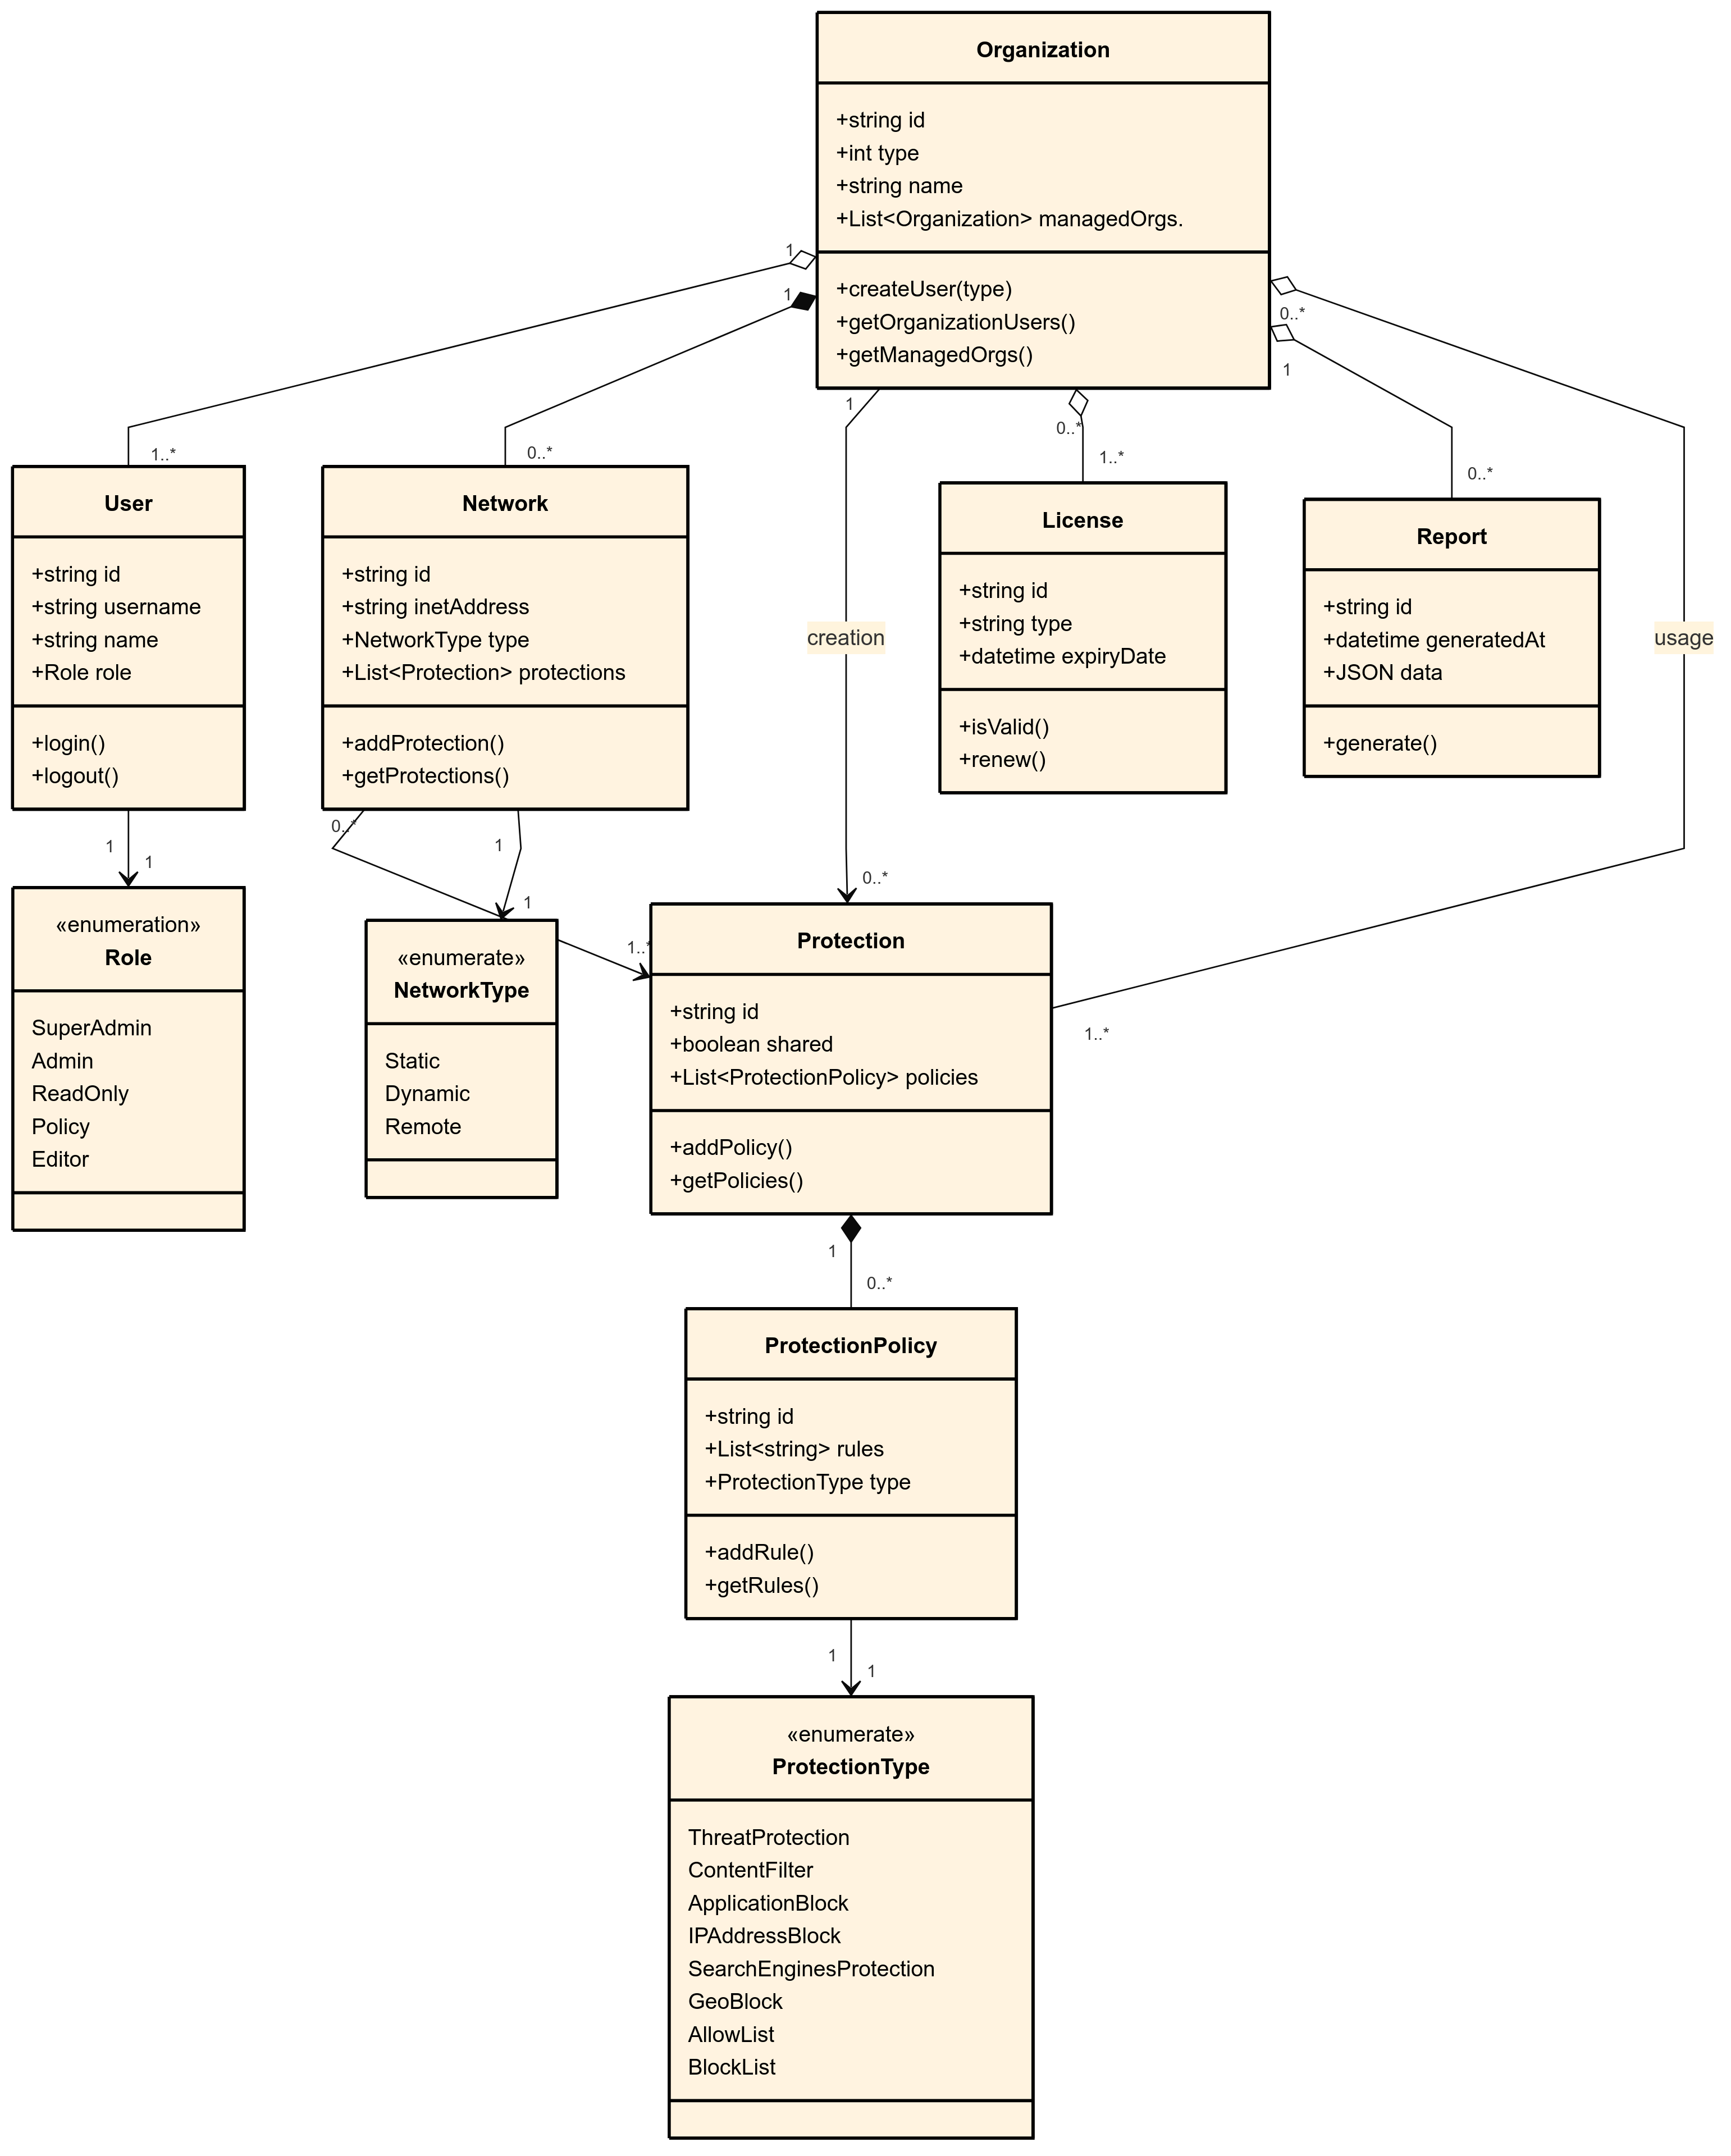
\includegraphics[width=1\textwidth]{figures/domain-model.png}
  \caption{Diagramma delle classi UML relativo al dominio applicativo del nuovo sistema.}
  \label{fig:domain_model}
\end{figure}

\subsubsection{Organization}
L'entità \texttt{Organization} rappresenta il fulcro del sistema multi-tenant ed è il punto di riferimento per tutte le altre componenti. Ogni utente, configurazione di filtraggio e reportistica è direttamente associata a un'organizzazione, che costituisce il contesto primario in cui avvengono le operazioni all'interno del sistema.

L'organizzazione è l'elemento che definisce l'esistenza stessa di un utente all'interno del sistema. Questi ultimi, infatti, non esistono al di fuori del contesto organizzativo: ogni utente deve appartenere a una specifica organizzazione e non può operare al di fuori di essa. Al momento della creazione di una nuova organizzazione, viene automaticamente generato un primo utente con permessi di amministratore. Tale amministratore ha la facoltà di creare nuovi utenti all'interno della propria organizzazione, o in quelle da essa gestite.

L'entità in questione non si limita a definire il perimetro degli utenti, ma è il nodo centrale attorno al quale ruotano tutte le altre configurazioni del sistema. Ogni organizzazione è associata a una o più reti (Network), che rappresentano gli indirizzi IP da sottoporre al filtraggio DNS. Le configurazioni di protezione (Protection), che definiscono cosa filtrare, sono legate all'organizzazione e non ai singoli utenti. Questo significa che tutte le policy di filtraggio sono decise a livello organizzativo. I dati statistici relativi all’utilizzo del sistema di filtraggio DNS sono raccolti e visualizzati a livello di organizzazione, consentendo agli utenti di monitorare il traffico filtrato e le attività correlate.

Ogni organizzazione è identificata da un \texttt{id} univoco, un nome (\texttt{name}) e una tipologia (\texttt{type}) che ne determina il ruolo all'interno del sistema. Esistono due macrotipologie di organizzazione:
\begin{itemize}
  \item \textbf{Organizzazioni che gestiscono altre organizzazioni}, ovvero Managed Service Provider e Dealer.
    \begin{itemize}
      \item \textbf{MSP}: oltre a rivendere il servizio di filtraggio DNS, si occupano direttamente della gestione della protezione per i loro clienti. In questo modello, il cliente finale non ha autonomia sulle proprie policy di protezione, in quanto è l'MSP a definirle e amministrarle.
      \item \textbf{Dealer}: rivendono il servizio di filtraggio DNS, ma senza occuparsi della configurazione delle policy. I clienti finali hanno piena libertà di gestione delle proprie protezioni.
    \end{itemize}
  \item \textbf{Clienti finali}, che possono essere:
    \begin{itemize}
      \item \textbf{Altre organizzazioni}, come scuole, hotel, aziende, attività commerciali.
      \item \textbf{Singoli individui}, che desiderano proteggere la propria rete domestica e i propri dispositivi personali.
    \end{itemize}
\end{itemize}

\subsubsection{User}
L'entità \texttt{User} rappresenta qualsiasi soggetto in grado di accedere al pannello di configurazione di un'organizzazione ed eseguire azioni sulla base dei permessi definiti dal proprio ruolo. Si ribadisce il fatto che gli utenti operano sempre all'interno del contesto di un'organizzazione, non potendo esistere in modo indipendente. Il sistema adotta un modello a ruoli per differenziare le capacità operative di ciascun utente, limitandone o ampliandone i privilegi a seconda delle necessità organizzative.

Esistono cinque tipologie di utenti, ciascuna con permessi specifici nell'ambito della propria organizzazione:
\begin{itemize}
  \item \textbf{SuperAdmin}: rappresenta l'utente con i più alti privilegi possibili. Questo ruolo è riservato al team di supporto dell'azienda produttrice del filtro DNS e gode di accesso illimitato a tutte le organizzazioni registrate nel sistema. Un SuperAdmin può creare ed eliminare utenti e organizzazioni, modificare qualsiasi policy e visionare tutti i report disponibili, indipendentemente dal cliente a cui sono associati.
  \item \textbf{Admin}: è l'utente amministratore della propria organizzazione e di tutte quelle al di sotto di essa nella gerarchia. Ha pieno controllo sulle entità amministrate ed è l'unico utente con il permesso di creare nuovi account all'interno del proprio contesto organizzativo.
  \item \textbf{Policy}: ha la facoltà di gestire le reti (Network) e i profili di protezione (Protection) all'interno della propria organizzazione. Non dispone di permessi amministrativi e non può gestire gli utenti.
  \item \textbf{Editor}: ha privilegi simili all'utente di tipo Policy, ma con un ambito più ristretto. In particolare, può gestire solo le configurazioni di sicurezza, senza poter modificare le impostazioni delle reti.
  \item \textbf{ReadOnly}: è l'utente con il livello di accesso più limitato. Ha esclusivamente il permesso di visionare report e statistiche, senza poter modificare alcuna configurazione. Il suo ruolo è strettamente legato al monitoraggio passivo delle attività del filtro DNS per una data organizzazione.
\end{itemize}

Ogni utente è identificato da un \texttt{id}, un nome (\texttt{name}), un ruolo (\texttt{role}) e da uno \texttt{username}. Quest'ultimo campo contiene l'indirizzo email dell'utente ed è utilizzato per l'autenticazione all'interno del sistema.

\subsubsection{License}
L'entità \texttt{License} rappresenta una delle componenti ancora in fase di modellazione, ma il suo ruolo nel sistema è chiaro: essa determina il livello di servizio del prodotto associato a un'organizzazione e influisce sui permessi e sulle funzionalità disponibili per quest’ultima. Ogni organizzazione deve disporre di almeno una licenza attiva per poter usufruire del servizio di filtraggio DNS.

Esistono diverse tipologie di licenze, tra cui quelle di prova, che vengono fornite gratuitamente con lo scopo di illustrare e dimostrare le capacità del prodotto prima di un eventuale acquisto. Oltre alle licenze di prova, sono previste licenze a pagamento con diversi livelli di servizio, i cui dettagli non sono ancora stati completamente definiti.

L'assegnazione di una licenza può essere effettuata esclusivamente da un utente con il ruolo di SuperAdmin, oppure dall’Admin di un’organizzazione di tipo MSP o Dealer. Ciò significa che solo il produttore del software e gli intermediari autorizzati possono concedere o modificare una licenza per un'organizzazione cliente.

\subsubsection{Report}
L'entità \texttt{Report} rappresenta la capacità del sistema di generare e visualizzare dati analitici relativi all'attività di filtraggio DNS per una o più organizzazioni. Lo scopo principale di un report è quello di fornire un monitoraggio dettagliato sull'utilizzo del filtro, offrendo statistiche utili per comprendere il traffico di rete e l'efficacia delle policy di protezione adottate. Tra le informazioni contenute in un report vi sono, ad esempio, il numero di richieste DNS bloccate, le cinque categorie di siti più frequentemente filtrate, il numero di domini non risolti e altri indicatori rilevanti per la sicurezza della rete.

Una caratteristica distintiva del nuovo sistema è la possibilità di generare report aggregati, che includono dati provenienti da più organizzazioni. Questa funzionalità è particolarmente utile per gli MSP, in quanto consente loro di ottenere una panoramica completa e centralizzata sui clienti che gestiscono. I report aggregati possono includere informazioni come l’elenco dei malware rilevati e i dispositivi su cui sono stati identificati, il numero di sessioni attive e altre metriche relative alla sicurezza e alla gestione del traffico DNS.

L'entità Report non è ancora stata completamente modellata, ma il suo ruolo nel sistema è fondamentale per garantire una visibilità chiara e approfondita sull’efficacia delle configurazioni di filtraggio applicate alle reti delle organizzazioni.

\subsubsection{Protection}
L'entità \texttt{Protection} rappresenta il concetto di protezione associato a una rete (Network), determinando in che modo il sistema di filtraggio DNS deve bloccare o consentire l'accesso ai contenuti. Ogni istanza di Protection è composta da una lista di policy di sicurezza, ognuna delle quali specifica una particolare configurazione del filtro. Generalmente, una Protection viene creata da un'organizzazione e assegnata a una o più delle proprie reti, definendo le regole di filtraggio applicate al traffico proveniente da tali indirizzi IP.

Con lo sviluppo del nuovo sistema, l’entità in esame introduce un'importante evoluzione: la possibilità di essere condivisa tra più organizzazioni. Se un’Organization crea una Protection e la contrassegna come condivisibile, tale configurazione potrà essere visualizzata e assegnata dai clienti gestiti dall'organizzazione creatrice. Questa funzionalità risulta particolarmente utile per gli MSP e i Dealer, che possono fornire ai propri clienti configurazioni predefinite e standardizzate senza richiedere loro di crearne di nuove.

Un ulteriore vantaggio del nuovo modello è la propagazione automatica delle modifiche per le Protection condivise. Se l’organizzazione creatrice aggiorna una configurazione di protezione condivisa, tutte le organizzazioni che la utilizzano vedranno applicate automaticamente le modifiche, senza necessità di intervento manuale. Per supportare questa logica, la modellazione prevede due relazioni distinte tra Protection e Organization:
\begin{enumerate}
  \item Una relazione di \textit{associazione semplice} che esprime la creazione, collegando un’Organization alla Protection che ha generato.
  \item Una relazione di \textit{aggregazione} che esprime l’utilizzo, collegando una Protection a una o più Organization che la utilizzano. Questa relazione è valida sia per le Protection non condivise, che per quelle condivise.
\end{enumerate}

Nonostante la sua importanza, Protection da sola non è sufficiente a garantire il livello di granularità richiesto da un moderno sistema di filtraggio DNS. Per questo motivo, essa è composta da una lista di configurazioni più specifiche, rappresentate dall'entità ProtectionPolicy, che definisce nel dettaglio il comportamento della protezione.

\subsubsection{ProtectionPolicy}
L'entità \texttt{ProtectionPolicy} rappresenta un insieme di regole appartenenti alla stessa tipologia di protezione, definita dall'attributo \texttt{ProtectionType}. Poiché il sistema di filtraggio DNS prevede diverse categorie di protezione, la modellazione adotta una struttura a due livelli: l'entità Protection mantiene la lista delle policy applicate, mentre ogni elemento di questa lista contiene le regole specifiche relative a una determinata categoria di protezione.
%
Questa suddivisione consente di organizzare in modo chiaro e modulare le configurazioni di sicurezza. Un'istanza di Protection può essere composta da più ProtectionPolicy, ciascuna responsabile di un particolare aspetto del filtraggio. Questo approccio permette alle organizzazioni di combinare diverse policy all'interno di un'unica configurazione di protezione, garantendo così una gestione flessibile e scalabile delle regole di filtraggio DNS.
%
I possibili tipi di protezione (\texttt{ProtectionType}) includono:
\begin{itemize}
  \item \textbf{ThreatProtection}: blocca siti identificati come minacce alla sicurezza, come malware e phishing.
  \item \textbf{ContentFilter}: filtra i contenuti sulla base della loro categoria tematica (es. pornografia, giochi d'azzardo, social network).
  \item \textbf{ApplicationBlock}: impedisce l’accesso a specifiche applicazioni o servizi online.
  \item \textbf{IPAddressBlock}: blocca l'accesso a determinati indirizzi IP.
  \item \textbf{SearchEnginesProtection}: applica restrizioni alle ricerche sui motori di ricerca, come l'attivazione forzata della modalità SafeSearch.
  \item \textbf{GeoBlock}: limita l’accesso a domini o indirizzi IP in base alla loro geolocalizzazione.
  \item \textbf{AllowList} e \textbf{BlockList}: definiscono eccezioni personalizzate, rispettivamente per consentire o bloccare domini specifici.
\end{itemize}

\subsubsection{Network}
L'entità \texttt{Network} riveste un ruolo fondamentale nel presente dominio applicativo, in quanto definisce l’ambito su cui devono essere applicate le regole di protezione del filtro DNS. Ogni rete è associata a un'Organization e rappresenta il punto di ingresso del traffico che verrà sottoposto a filtraggio. La configurazione della protezione di una rete è determinata dalla Protection assegnata ad essa, specificando così quali policy devono essere applicate.
%
Questa relazione tra Network e Organization è modellata come una \textit{composizione}, indicando che una rete non può esistere senza l’Organization a cui appartiene. Se un'organizzazione viene eliminata, anche tutte le reti ad essa associate vengono rimosse.

Una rete può appartenere a una delle seguenti tipologie, identificate dall'enumerazione \texttt{NetworkType}:
\begin{itemize}
  \item \textbf{Static}: identifica reti con un indirizzo IP statico, il cui riferimento rimane invariato nel tempo.
  \item \textbf{Dynamic}: rappresenta reti con indirizzo IP dinamico, che necessitano dell’ausilio di un servizio di DynamicDNS per garantire un'associazione stabile nel tempo.
  \item \textbf{Remote}: utilizzata per proteggere dispositivi mobili ed endpoint aziendali che richiedono la protezione del filtro DNS anche quando non sono connessi alla rete principale dell'organizzazione.
\end{itemize}

Ogni Network è identificata da un \texttt{id}, da un \texttt{type} e da un \texttt{inetAddress}. Quest'ultimo supporta sia indirizzi IPv4 che IPv6 e consente l'inserimento di intervalli IP secondo lo standard Classless Inter-Domain Routing\footnote{\url{https://datatracker.ietf.org/doc/html/rfc4632}} (CIDR), specificandoli con una barra finale (es. \texttt{192.168.1.0/24}). L'associazione tra Network e Protection permette di applicare un insieme di policy a una specifica rete, garantendo così un controllo granulare sul filtraggio del traffico DNS.

\chapter{Design}

Il presente capitolo descrive le scelte architetturali, tecnologiche e progettuali adottate per soddisfare gli obiettivi e i requisiti definiti nel capitolo precedente. L'attenzione si concentra sulle funzionalità sviluppate o analizzate durante il tirocinio, pur accennando alle linee guida per alcune delle funzionalità future, al fine di offrire una visione più completa del sistema.

La progettazione del nuovo sistema punta a superare i limiti identificati nel legacy, adottando un'architettura moderna, modulare e scalabile, che semplifichi la gestione e consenta l'integrazione di nuove funzionalità. Particolare attenzione è stata dedicata alla separazione delle responsabilità tra i vari componenti, alla progettazione di un backend flessibile e robusto agli errori, e alla realizzazione di un frontend intuitivo e con un aspetto enterprise.

Il capitolo è strutturato come segue: dopo una descrizione dell’architettura generale del sistema, si approfondiranno le principali componenti e funzionalità chiave, come la multiutenza e la gestione degli errori. Infine, saranno discussi gli aspetti relativi al miglioramento del database e alle strategie messe in campo per garantire una corretta migrazione dei dati dal sistema legacy.

\section{Architettura generale}
Per la progettazione del nuovo sistema è stata adottata un'architettura a microservizi, caratterizzata da una separazione netta tra frontend e backend. Questa scelta è motivata dalla necessità di superare i limiti architetturali del sistema legacy, introducendo modularità e una chiara separazione delle responsabilità tra i vari componenti.

Nel nuovo sistema, il frontend è rappresentato da un singolo microservizio dedicato alla logica di presentazione dei dati e all'interazione con l'utente. Il backend, invece, è stato suddiviso in molteplici microservizi indipendenti, ciascuno dedicato a un modulo o a una funzionalità specifica dell'applicativo. Questa scomposizione consente di ottenere una maggiore flessibilità, facilitando sia l'aggiunta di nuove funzionalità che la manutenzione del sistema.

I microservizi comunicano tra loro utilizzando il protocollo HTTP e, più specificamente, attraverso le API RESTful che ciascuno di essi espone. Queste ultime vengono inoltre utilizzate sia dal frontend sia per la creazione delle API pubbliche aziendali. Tali API, già presenti insieme al sistema legacy, sono state rinnovate per adattarsi alle nuove logiche di funzionamento introdotte nel nuovo sistema.

Una rappresentazione schematica dell'architettura del sistema è riportata in \Cref{fig:system-architecture}, dove sono evidenziate le principali componenti del frontend e del backend. Il diagramma mostra come il primo gestisca l'interazione con l'utente attraverso moduli specifici per il routing e per la gestione dello stato e della sessione, mentre il secondo sia organizzato in servizi dedicati a funzionalità come gestione utenti e autenticazione.

\begin{figure}
  \centering
  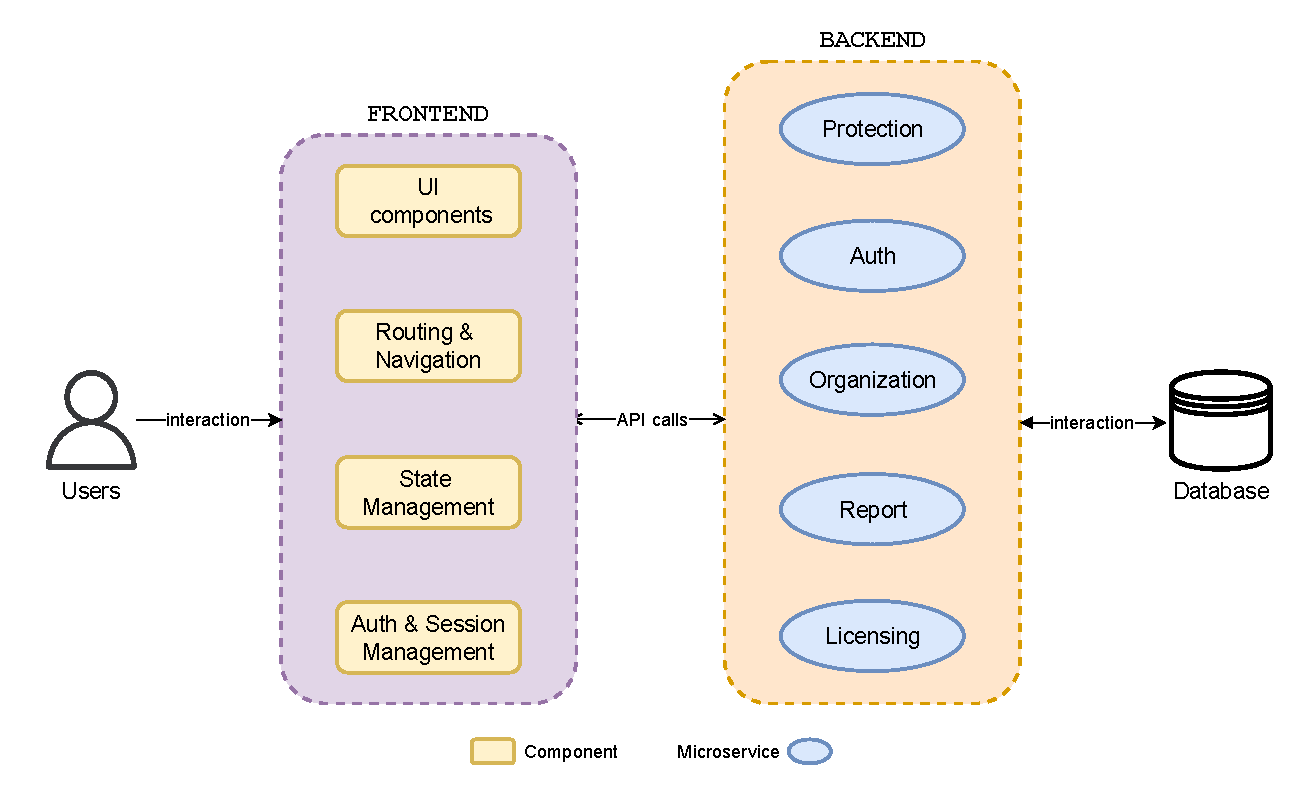
\includegraphics[width=1\textwidth]{figures/system-architecture.pdf}
  \caption{Architettura generale del sistema.}
  \label{fig:system-architecture}
\end{figure}

\subsection{Struttura del Frontend}
Il frontend è stato progettato come una Single-Page Application (SPA) \cite{Fink2014}, scelta che consente di offrire agli utenti un'esperienza fluida e un accesso rapido da qualsiasi browser, senza bisogno di installare alcun applicativo localmente. Questo microservizio si occupa esclusivamente della logica di presentazione, implementando l'interfaccia grafica e gestendo l'interazione con gli utenti finali. Infatti, tutte le operazioni di elaborazione dei dati, come le computazioni o la gestione delle regole di business, sono demandate al backend.

L'architettura del frontend segue un approccio modulare, in cui ogni pagina e componente è organizzato secondo una struttura gerarchica. Ciò consente di mantenere l'architettura chiara e scalabile, facilitando l'estensione del sistema e la gestione delle singole sezioni dell'applicazione.

Per garantire un design coerente e accelerare lo sviluppo dell'interfaccia, è stato adottato un template grafico altamente personalizzabile. Questo approccio ha consentito di ridurre i tempi di progettazione dell’interfaccia grafica, mantenendo al contempo la flessibilità necessaria per adattare l’aspetto grafico alle esigenze specifiche del progetto.

\subsection{Struttura del Backend}
Come già accennato, il backend non è stato concepito come un unico servizio monolitico, ma si è optato per una suddivisione in più microservizi, ciascuno responsabile di una specifica funzionalità o modulo del sistema. La definizione di questi microservizi è stata guidata dall'analisi del dominio (\Cref{sec:domain-analysis}), individuando le principali entità e le loro responsabilità all'interno dell'architettura complessiva. Questo approccio ha permesso di modellare il backend in modo coerente con le esigenze del sistema, garantendo una chiara separazione delle responsabilità e facilitando l'evoluzione futura della piattaforma. Di seguito, vengono descritti i principali microservizi di cui il backend è composto.

\paragraph{Auth}
Il microservizio \texttt{auth} è responsabile dell'autenticazione e dell'autorizzazione degli utenti. L'autenticazione è implementata attraverso un meccanismo basato su token, che consente di gestire sessioni sicure senza la necessità di mantenere uno stato lato server.
L'autorizzazione, invece, fornisce un sistema per determinare se un utente ha i permessi necessari per eseguire una determinata azione. Questa valutazione si basa sul ruolo dell'utente e sulla licenza associata all'organizzazione cui appartiene, garantendo così un controllo granulare sugli accessi alle funzionalità della piattaforma.

\paragraph{Report}
Il microservizio \texttt{report} gestisce la generazione e la visualizzazione dei report relativi alle attività di filtraggio DNS. Nella prima versione del sistema, questa funzionalità è limitata alla visualizzazione di report specifici per gli MSP. Questo microservizio si interfaccia con il database per raccogliere e aggregare i dati necessari, fornendo agli utenti una panoramica dettagliata sull'attività di filtraggio e sull'efficacia delle policy applicate.

\paragraph{Organization}
Il microservizio \texttt{organization} è un componente chiave per l'implementazione della multiutenza. Esso si occupa di gestire tutte le operazioni CRUD sugli utenti, consentendo di creare nuovi account, modificarne i dati, nonché rimuovere utenti dalle organizzazioni. Grazie a questo servizio più utenti possono essere associati a un'unica organizzazione con livelli di accesso differenziati, migliorando la flessibilità e la gestione delle autorizzazioni.

\paragraph{Protection}
Il microservizio \texttt{protection} è responsabile della gestione delle policy di protezione applicate agli utenti e alle organizzazioni. Questo servizio permette di creare, modificare ed eliminare i profili di protezione, ossia insiemi di regole che determinano quali contenuti possono essere filtrati o consentiti.
Inoltre, gestisce la creazione e l’amministrazione dei profili condivisi, che consentono di applicare una configurazione comune a più clienti senza dover definire manualmente le stesse regole per ciascuno di essi.

\paragraph{Licensing}
Il microservizio \texttt{licensing} si occupa della gestione delle licenze associate agli utenti e alle organizzazioni. Attraverso questo servizio, è possibile visualizzare lo stato delle licenze attive, gestire le assegnazioni e monitorare la loro scadenza.
Questo microservizio è essenziale per garantire che ogni utente abbia accesso solo alle funzionalità previste dal proprio piano, permettendo un controllo efficace sui livelli di servizio offerti.

\subsubsection{Architettura a livelli}
I microservizi appena discussi adottano un'architettura uniforme, basata sull'esposizione di API REST, garantendo una progettazione modulare e scalabile. Tale struttura consente di mantenere indipendenti le diverse componenti del sistema, facilitando la manutenzione e l'evoluzione del software. Ogni microservizio è organizzato in più livelli, ciascuno con responsabilità ben definite, come illustrato in \Cref{fig:microservice-architecture}:

\begin{itemize}
  \item \textbf{Routes}: rappresenta il punto di ingresso delle richieste HTTP. Questo livello si occupa di applicare eventuali middleware, come quello per la gestione dell'autenticazione, e di indirizzare le richieste verso il controller appropriato, in base al metodo HTTP e al percorso richiesto.

  \item \textbf{Controllers}: ricevono le richieste dai Routes, validano i parametri in ingresso e delegano l'elaborazione ai servizi applicativi. Una volta ottenuto il risultato, i controllers generano la risposta HTTP da restituire al client.

  \item \textbf{Services}: costituiscono il livello di business logic, elaborando i dati e orchestrando le operazioni necessarie. Questo livello intermedio permette di mantenere separata la logica di dominio dall'accesso ai dati, garantendo maggiore modularità e riusabilità del codice.

  \item \textbf{Repositories}: forniscono un'interfaccia per l'accesso ai dati, eseguendo operazioni di lettura e scrittura sul database. Questo livello è responsabile esclusivamente della gestione dei dati.

  \item \textit{Database}: sebbene non sia parte integrante dell'architettura dei microservizi, rappresenta il livello di persistenza su cui vengono eseguite le operazioni di lettura e scrittura da parte dei repositories.
\end{itemize}

\begin{figure}
  \centering
  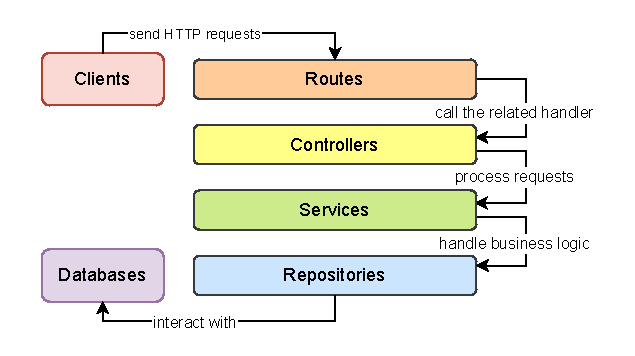
\includegraphics[width=0.9\textwidth]{figures/microservice-architecture.pdf}
  \caption{Visione schematica relativa all'architettura a livelli dei microservizi.}
  \label{fig:microservice-architecture}
\end{figure}
%
Questa suddivisione in livelli garantisce una chiara separazione delle responsabilità, migliorando la manutenibilità e la scalabilità del sistema. Inoltre, consente di evolvere il backend in modo strutturato, rendendo più semplice l'aggiunta di nuove funzionalità o modifiche alle logiche applicative senza impattare gli altri componenti.

\subsection{Interazione tra i componenti}
La comunicazione tra i componenti del sistema avviene principalmente tramite chiamate HTTP verso un'API, permettendo al frontend, e ai microservizi del backend, di interagire in maniera modulare ed efficiente. In \Cref{fig:system-interactions} è rappresentata la struttura generale del sistema, evidenziando i flussi di comunicazione tra frontend, backend e database, oltre alle interazioni tra i microservizi del backend.

\begin{figure}
  \centering
  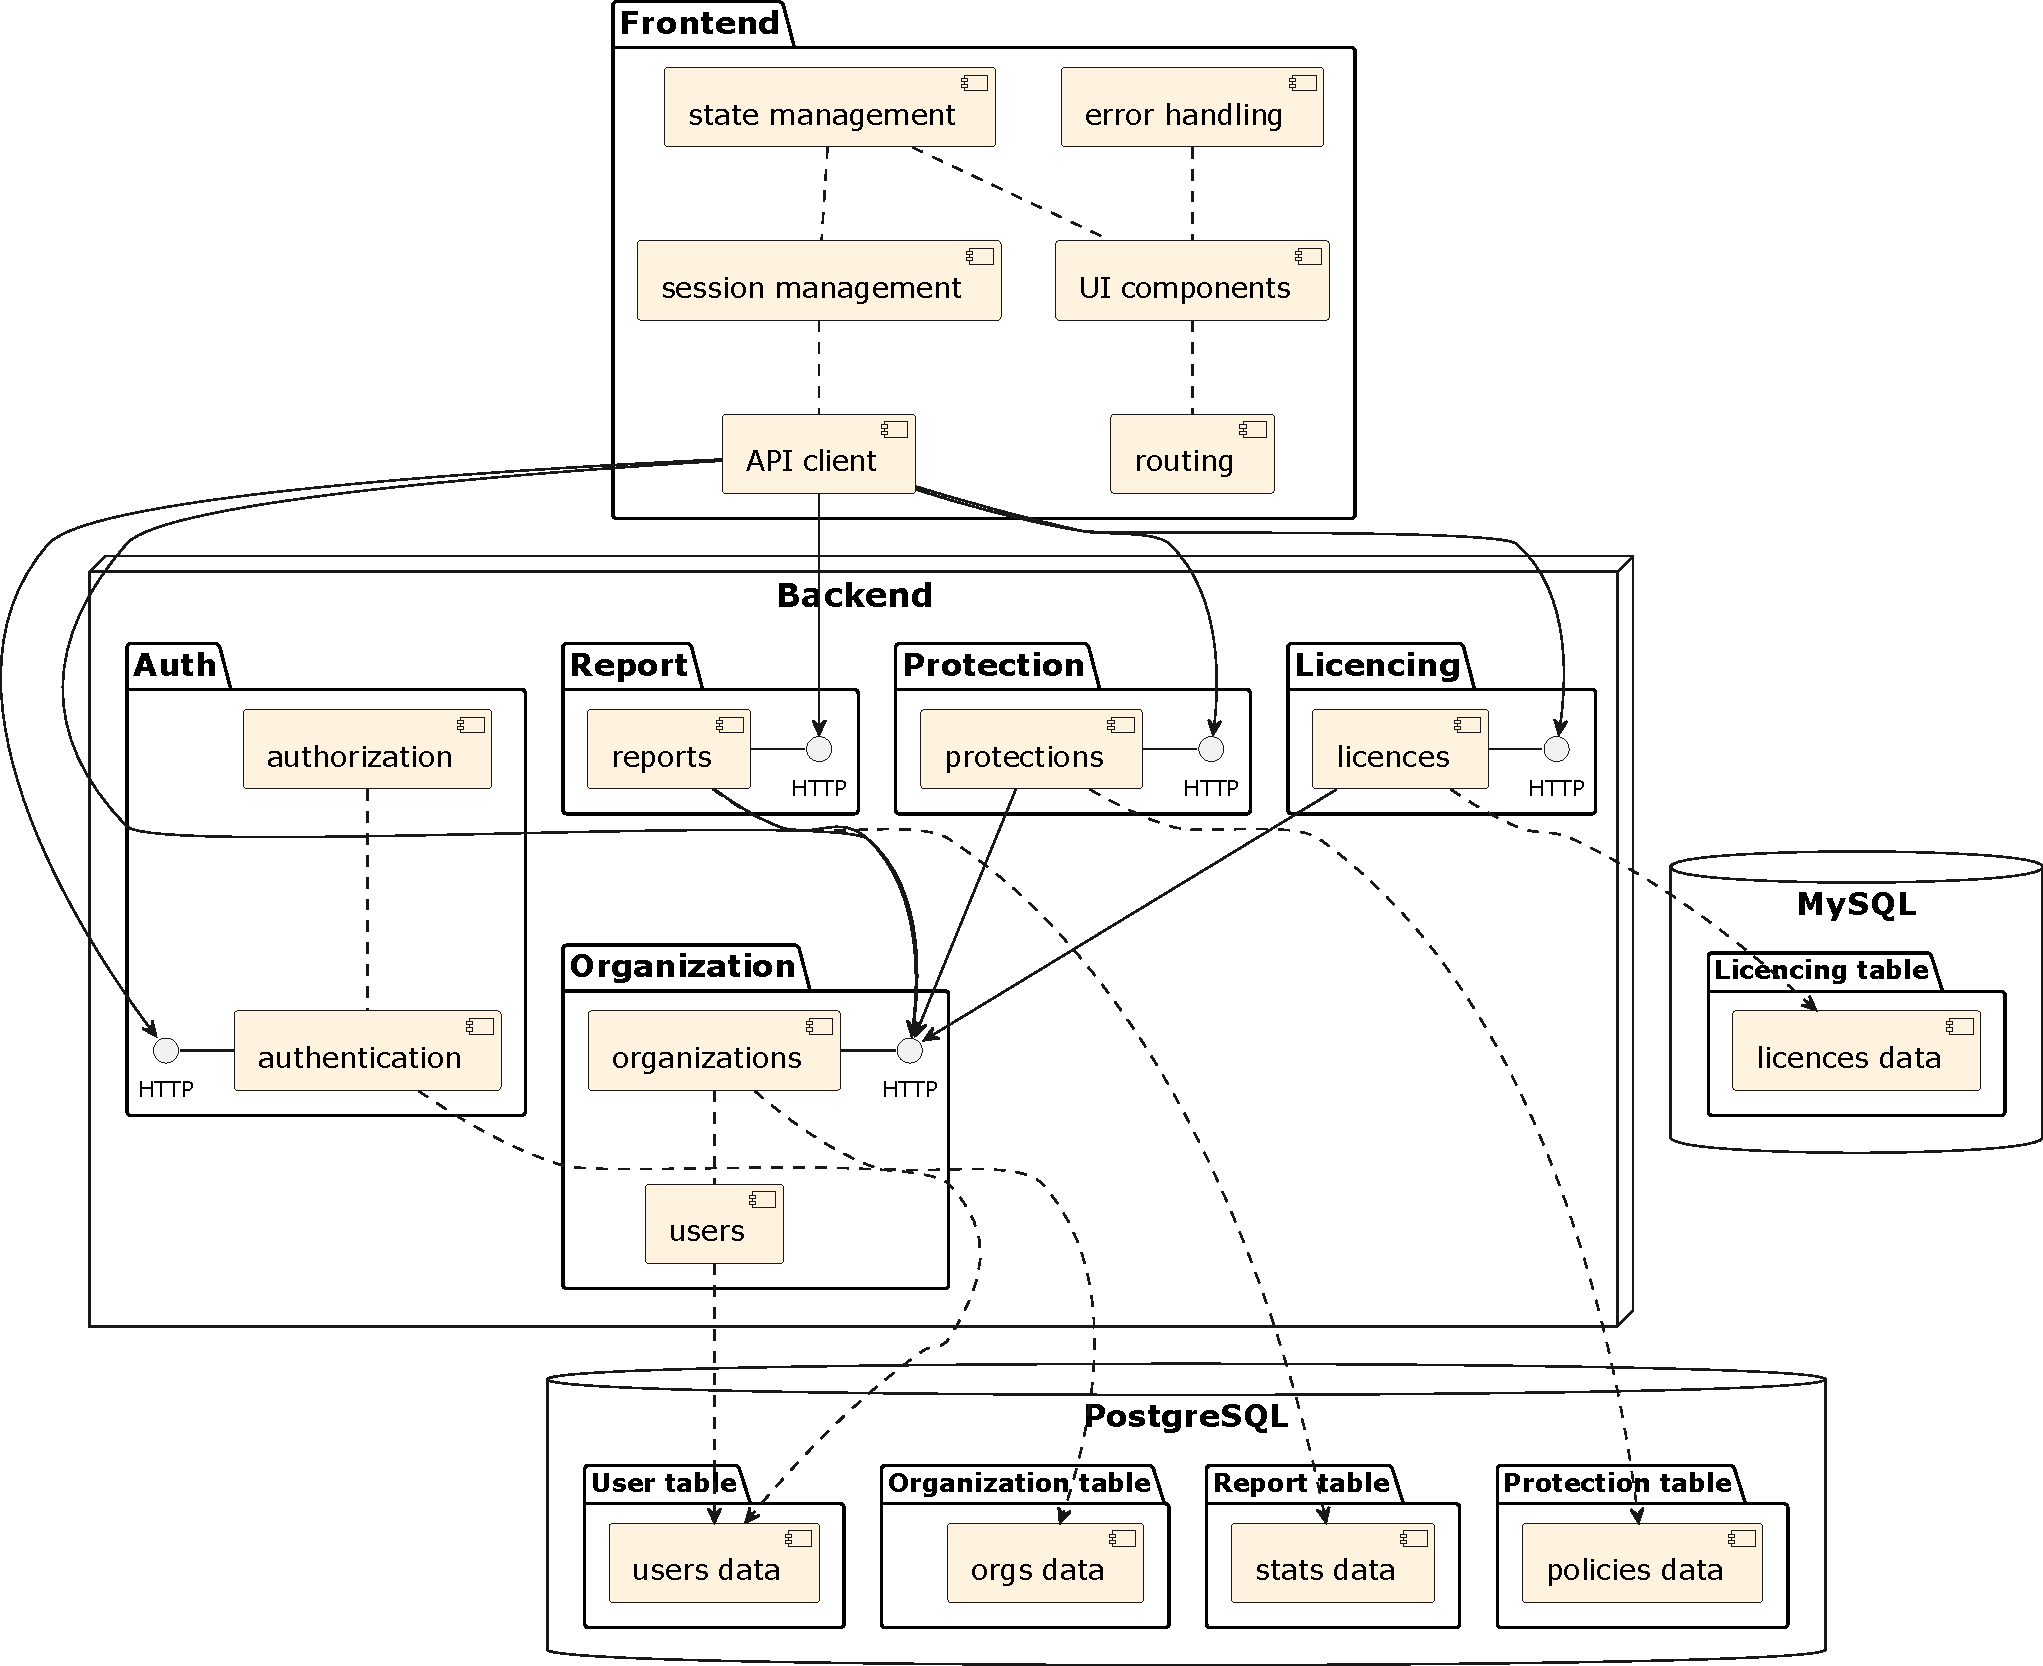
\includegraphics[width=1\textwidth]{figures/global-system-interactions.pdf}
  \caption{Visione globale del sistema relativamente ai suoi componenti e alle interazioni tra di essi.}
  \label{fig:system-interactions}
\end{figure}

\subsubsection{Componenti e interazioni del frontend}
Sebbene il frontend sia implementato come un unico microservizio, al suo interno è suddiviso in moduli funzionali che si occupano di gestire aspetti specifici dell’interfaccia utente e della comunicazione con il backend. Tra i principali:
\begin{itemize}
  \item \textbf{Routing e navigazione}: gestisce il passaggio tra le diverse viste dell'applicazione.
  \item \textbf{Gestione dello stato}: mantiene e sincronizza le informazioni tra i componenti per garantire coerenza nei dati.
  \item \textbf{Autenticazione e sessione}: protegge le sezioni riservate e gestisce l’accesso degli utenti.
  \item \textbf{Client API}: funge da intermediario tra il frontend e il backend, inviando richieste e processando le risposte.
  \item \textbf{Gestione degli errori}: intercetta eventuali problemi nelle comunicazioni con il backend e fornisce all'utente un feedback chiaro.
\end{itemize}

% Il frontend interagisce con il backend esclusivamente tramite chiamate API REST, delegando a esso l'elaborazione dei dati e la logica applicativa.

\subsubsection{Interazioni del backend}
Come è già stato puntualizzato, i microservizi del backend comunicano tra loro, e con il frontend, esponendo API REST. Ogni servizio è progettato per gestire una specifica funzionalità e può interagire con gli altri quando necessario. Le principali interazioni avvengono secondo due modalità:
\begin{itemize}
  \item \textbf{Comunicazione frontend-backend}: il frontend invia richieste ai microservizi per ottenere dati o eseguire operazioni, ricevendo le informazioni necessarie per aggiornare l'interfaccia utente.
  \item \textbf{Interazioni tra microservizi}: i servizi si scambiano dati tramite API REST per operazioni che coinvolgono più moduli, come la gestione degli utenti, delle organizzazioni o delle policy di protezione.
\end{itemize}

Questo modello garantisce che ogni microservizio operi in modo indipendente, riducendo le dipendenze dirette e migliorando la scalabilità e l'efficienza complessiva del sistema.

\subsubsection{Interazione con i database}
Il backend sfrutta due database distinti per la gestione della persistenza dei dati:
\begin{itemize}
  \item \textbf{PostgreSQL}: utilizzato per la maggior parte delle operazioni, inclusa la gestione di utenti, organizzazioni, report, autenticazione e policy di protezione.
  \item \textbf{MySQL}: impiegato esclusivamente per la gestione delle licenze, in quanto derivante dal sistema legacy. Il pannello customer area utilizza questo database per archiviare e gestire le licenze dei clienti.
\end{itemize}

\subsubsection{Interazione tra i livelli interni del backend}
Come già menzionato, ogni microservizio del backend segue un'architettura a livelli ben definita, composta da \textit{Routes}, \textit{Controllers}, \textit{Services} e \textit{Repositories}. Tuttavia, non è stato ancora approfondito il modo in cui questi livelli interagiscono tra loro e come questa struttura influenzi il funzionamento complessivo del sistema.

L'organizzazione a livelli permette di mantenere una chiara separazione delle responsabilità, semplificando la manutenzione e l'estensibilità del software. La \Cref{fig:microservice-internal-interactions} illustra il flusso di interazione tra questi componenti, evidenziando il percorso di una richiesta all'interno del sistema, dal momento in cui viene ricevuta fino alla gestione dei dati nel livello di persistenza.

\begin{figure}
  \centering
  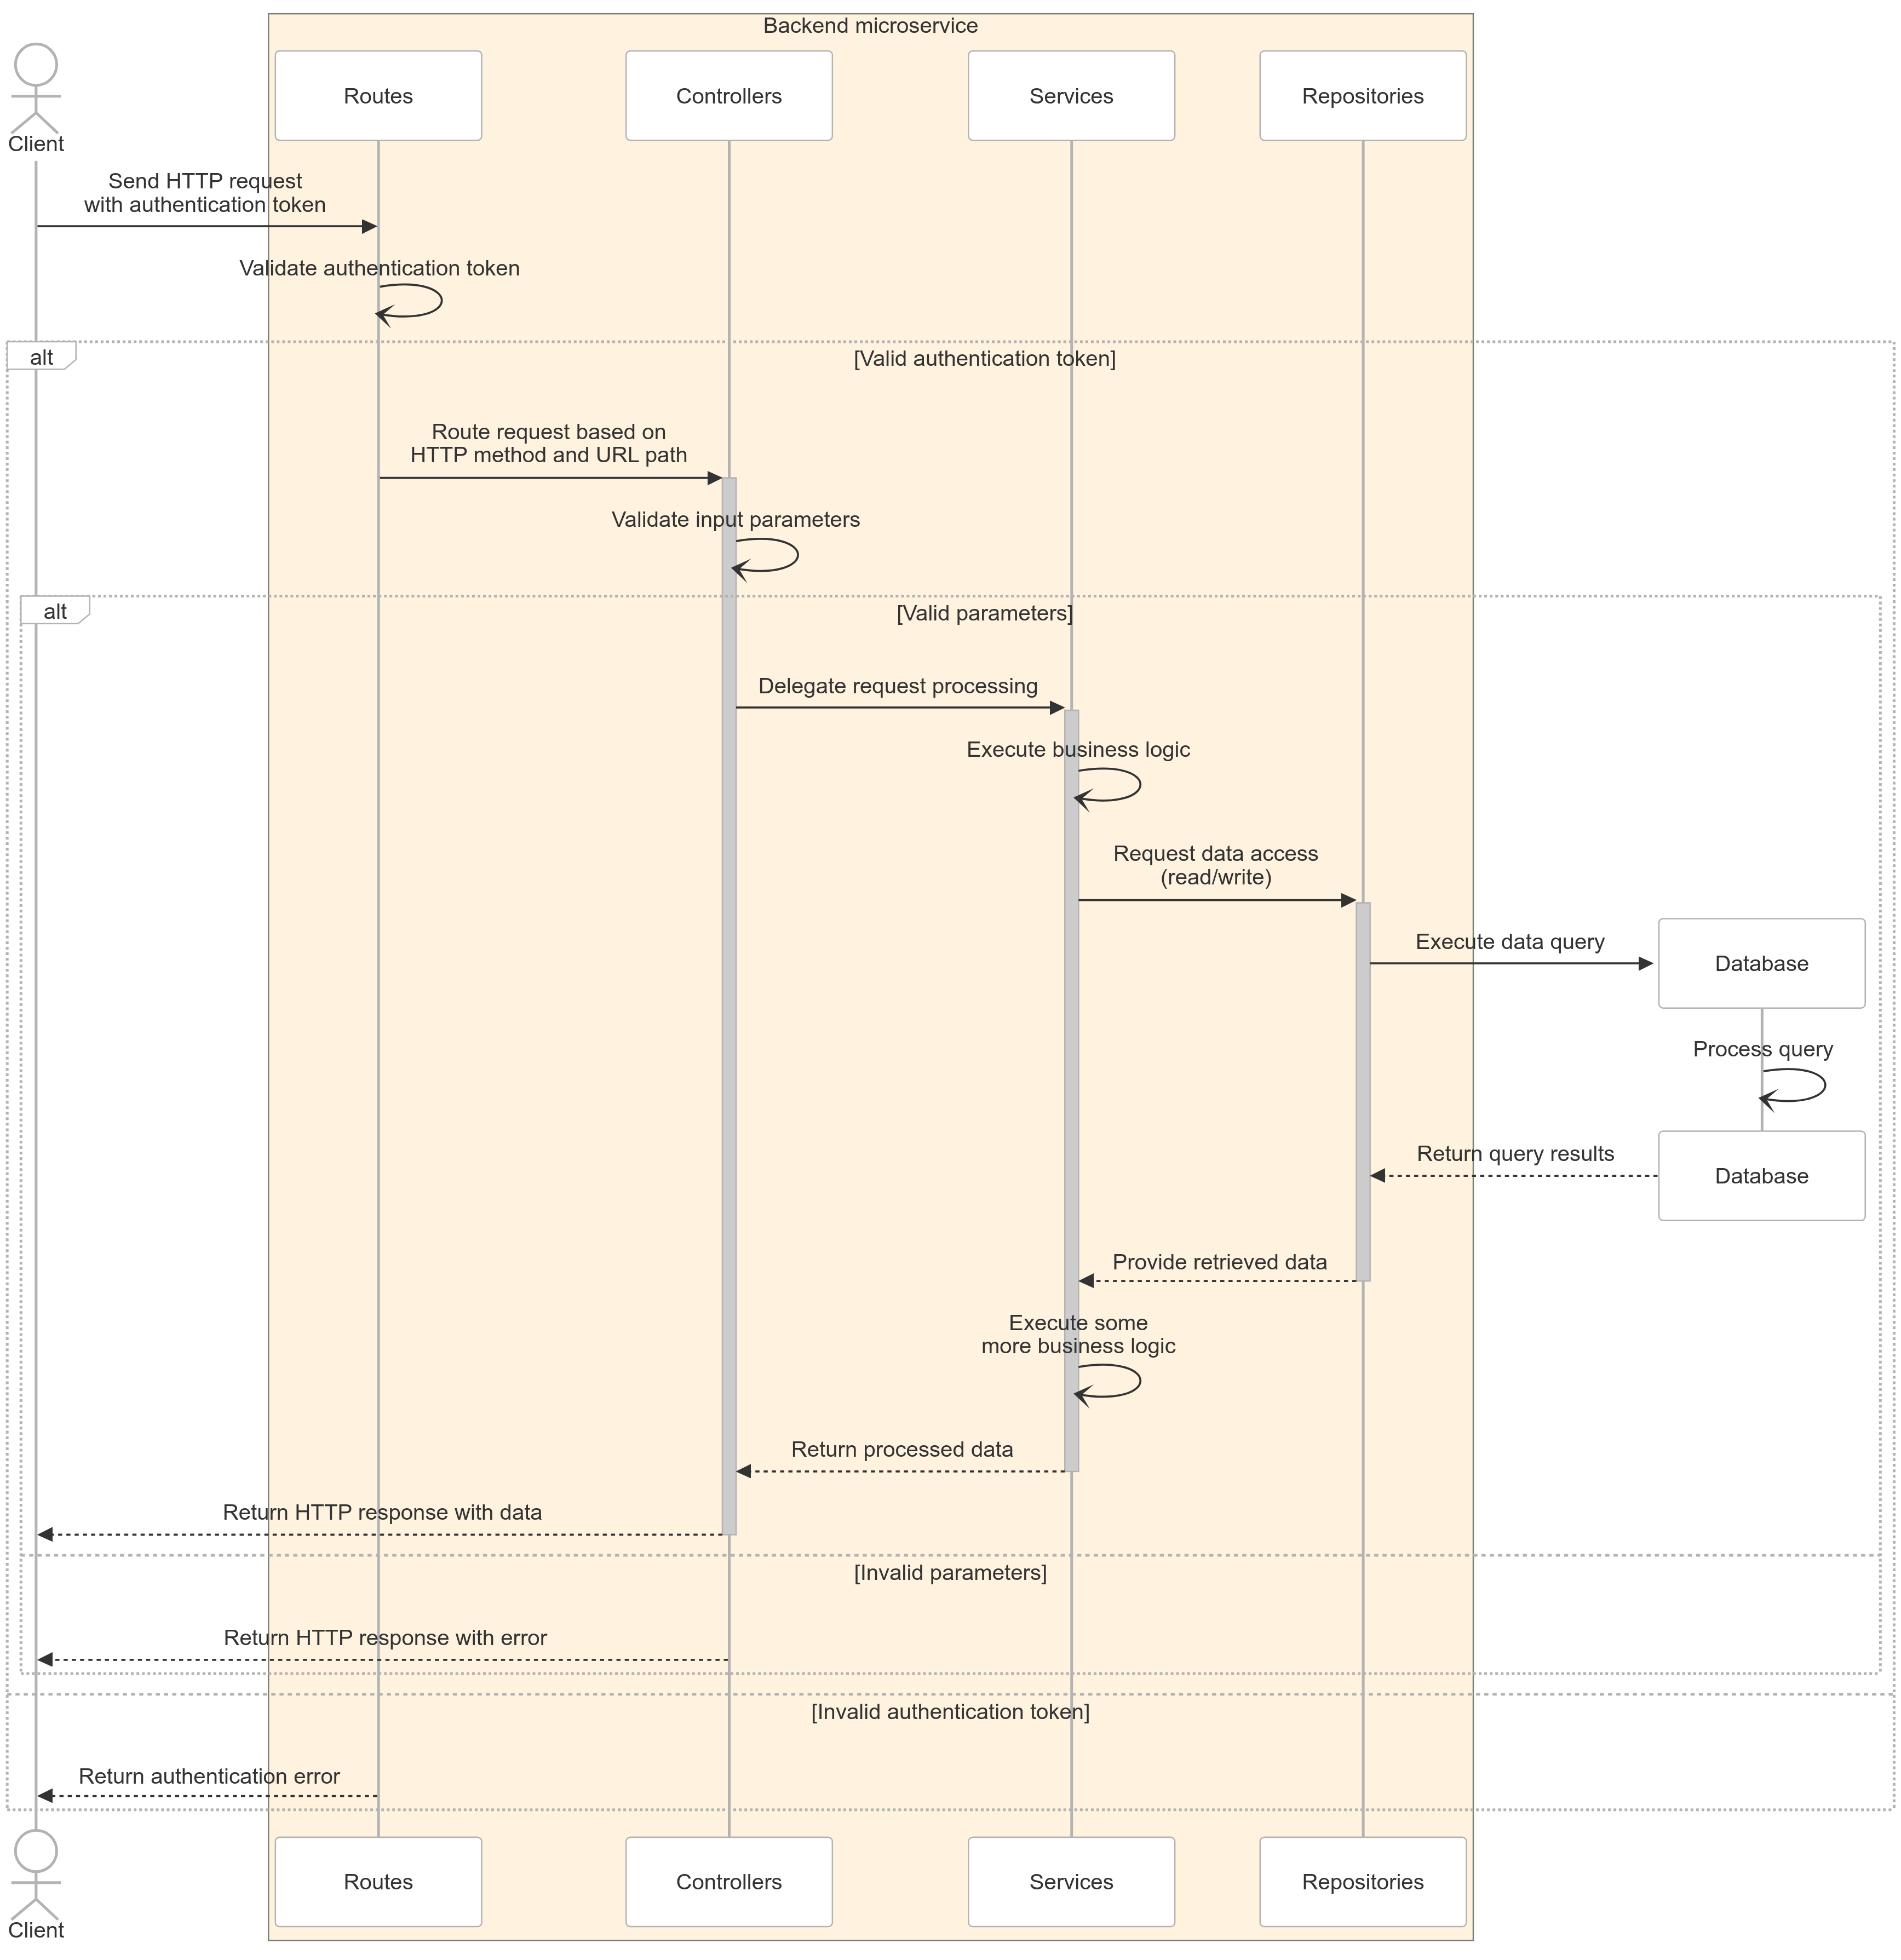
\includegraphics[width=1\textwidth]{figures/microservice-internal-interactions.png}
  \caption{Diagramma di sequenza UML che illustra l'interazione tra i livelli dell'architettura interna del backend.}
  \label{fig:microservice-internal-interactions}
\end{figure}

Il processo inizia quando un client invia una richiesta HTTP al backend, includendo eventualmente un token di autenticazione. Il primo livello che intercetta la richiesta è quello delle \textit{Routes}, che ha il compito di validare il token e determinare il controller appropriato in base al metodo HTTP e al percorso della richiesta. Se il token di autenticazione non è valido, il sistema risponde immediatamente con un errore.
%
Al contrario, se il processo di autenticazione va a buon fine, la richiesta viene inoltrata al livello dei \textit{Controllers}, che ha la responsabilità di verificare la correttezza dei parametri in ingresso. Se i parametri risultano non validi, viene generata una risposta di errore senza procedere oltre. In caso contrario, il controller delega l'elaborazione della richiesta al livello \textit{Services}.
%
I servizi rappresentano il cuore della logica di business del sistema. Qui vengono eseguite le operazioni necessarie per soddisfare la richiesta, che possono includere accessi ai dati. Se è necessario recuperare o modificare informazioni persistenti, il servizio delega l'operazione al livello dei \textit{Repositories}, il quale è responsabile della comunicazione diretta con il database. Esso esegue le query richieste e restituisce i risultati al servizio chiamante. Quest'ultimo può applicare ulteriori elaborazioni ai dati ricevuti prima di restituirli al controller.
%
Infine, il controller invia la risposta direttamente al client, restituendo i dati elaborati o, in caso di errore, un messaggio appropriato. Questo flusso strutturato garantisce un'elevata modularità del backend, facilitando l'estensione del sistema e migliorando la gestione degli errori e della sicurezza.

\subsection{Scelte tecnologiche}
Le tecnologie utilizzate per l'implementazione del nuovo sistema erano già state definite prima dell'inizio del presente lavoro di tesi. Tuttavia, la loro adozione può essere motivata sulla base di considerazioni tecniche e di opportunità.

Per l'intero sistema, sia frontend che backend, è stato scelto il linguaggio TypeScript\footnote{\url{https://www.typescriptlang.org}}, che combina la flessibilità e la vasta disponibilità di librerie di JavaScript con i vantaggi di un linguaggio tipizzato. Grazie a TypeScript, è stato possibile sviluppare entità e funzionalità più robuste rispetto a un'implementazione in JavaScript puro, riducendo il rischio di errori a runtime. Il sistema di tipizzazione consente di individuare molteplici errori già in fase di compilazione, generando file JavaScript più affidabili e sicuri.

Come sistema di gestione delle dipendenze, si è optato per \texttt{pnpm}\footnote{\url{https://pnpm.io}}, un package manager che offre un'alternativa più efficiente rispetto ai classici \texttt{npm} o \texttt{yarn}. Questo strumento si distingue per la sua capacità di ottimizzare l'uso dello spazio su disco condividendo le dipendenze tra i progetti, evitando duplicazioni inutili e riducendo significativamente i tempi di installazione. Inoltre, garantisce una gestione più affidabile delle dipendenze grazie al meccanismo di \textit{store globale}, che assicura un'integrità maggiore rispetto agli altri gestori. La scelta di \texttt{pnpm} è stata adottata in maniera uniforme per garantire coerenza tra frontend e backend, migliorando l'efficienza del processo di sviluppo.

\subsubsection{Tecnologie del frontend}
Il frontend è stato sviluppato utilizzando Next.js\footnote{\url{https://nextjs.org}}, un framework basato su React. La scelta di React\footnote{\url{https://react.dev}} è stata dettata dalla volontà di mantenere la filosofia del sistema legacy, che forniva il pannello sotto forma di web application, e dalla sua combinazione tra ampia diffusione, efficienza e curva di apprendimento bilanciata. Tuttavia, piuttosto che utilizzare React in modo standalone, si è preferito adottare un framework che ne ottimizzasse l’utilizzo. Next.js è stato selezionato per le sue funzionalità avanzate, tra cui il pieno supporto a TypeScript e la gestione automatizzata di operazioni come il bundling e la compilazione, consentendo agli sviluppatori di concentrarsi sulla logica applicativa senza preoccuparsi della configurazione dell'ambiente di sviluppo.

Come strategia di routing delle pagine, si è scelto di utilizzare App Router\footnote{\url{https://nextjs.org/docs/app}}, il sistema di routing integrato in Next.js. Questo approccio permette di definire le rotte dell'applicazione in modo strutturato, organizzando il codice in base alla gerarchia delle directory. Inoltre, offre supporto per il rendering lato server, migliorando la flessibilità nella gestione e nel caricamento dei componenti.

Dal punto di vista grafico, la scelta del template TailAdmin\footnote{\url{https://tailadmin.com}} come base di partenza è stata motivata dalla sua somiglianza con il design desiderato per il nuovo sistema. La disponibilità di schermate predefinite e componenti riutilizzabili ha accelerato lo sviluppo dell’interfaccia, mentre la sua natura open source ha garantito massima flessibilità, permettendo modifiche e personalizzazioni senza vincoli.

\subsubsection{Tecnologie del backend}
Tutti i microservizi del backend utilizzano il framework web Express\footnote{\url{https://expressjs.com}} per esporre le loro API REST. Questa scelta è stata dettata dalla leggerezza e rapidità di tale libreria, oltre alla sua capacità di gestire le rotte in modo intuitivo e modulare. Express consente di definire una gerarchia di routing chiara, facilitando la suddivisione delle responsabilità tra i vari livelli dell'architettura. Inoltre, supporta l'integrazione di middleware personalizzati, aumentando la flessibilità nella gestione delle logiche applicative, come l'autenticazione e la validazione delle richieste.

Per i meccanismi di autenticazione, si è optato per un sistema basato su JSON Web Token\footnote{\url{https://datatracker.ietf.org/doc/html/rfc7519}} (JWT). Questa soluzione è ampiamente diffusa grazie alla sua semplicità di implementazione e alla possibilità di essere utilizzata in ambienti scalabili e distribuiti senza la necessità di mantenere uno stato centralizzato per le sessioni utente. A condizione che venga implementata correttamente, JWT garantisce un elevato livello di sicurezza, permettendo un controllo efficiente sugli accessi e l'integrazione con i microservizi in maniera indipendente.

Per quanto riguarda la gestione dell’accesso ai dati, si è scelto di adottare un Object-Relational Mapping  (ORM) per semplificare l’interazione tra il backend e il database, evitando la necessità di scrivere manualmente query SQL all’interno del codice applicativo. In particolare, la scelta è ricaduta su Prisma\footnote{\url{https://www.prisma.io}}, che si differenzia dagli Object-Relational Mapping tradizionali per il suo approccio dichiarativo. Più in dettaglio, a differenza degli ORM convenzionali, che mappano le tabelle del database su classi del linguaggio di programmazione, Prisma utilizza uno schema dichiarativo chiamato \textit{Prisma Schema} come unica fonte di verità per la struttura del database e dei modelli dell’applicazione. Questo consente una gestione più chiara e coerente dei dati, evitando le problematiche legate all'incompatibilità tra il modello a oggetti e quello relazionale.
%
Dal punto di vista della programmazione, Prisma fornisce una libreria lato client che permette di eseguire operazioni di lettura e scrittura sul database in modo tipizzato e sicuro, senza la necessità di gestire manualmente istanze di modelli complessi.

\subsubsection{Scelte tecnologiche del database}
Il nuovo sistema adotta un database relazionale con tecnologia PostgreSQL, scelta dettata principalmente dalla necessità di garantire la compatibilità con i dati gestiti dal sistema legacy, che utilizza lo stesso DBMS. Oltre a questo requisito, PostgreSQL è stato selezionato per le sue caratteristiche di affidabilità, scalabilità e performance, rendendolo una soluzione solida per applicazioni che devono gestire un elevato volume di dati e richieste concorrenti.

\section{Aspetti funzionali del sistema}
Il sistema in esame implementa diverse funzionalità fondamentali per garantire un'esperienza utente efficiente e una gestione strutturata delle operazioni. Tra queste, la multiutenza consente di amministrare utenti con permessi differenziati, assicurando un controllo granulare sull’accesso alle risorse. Parallelamente, la gestione degli errori è stata progettata per migliorare l'affidabilità del sistema, garantendo un trattamento coerente e strutturato delle anomalie, sia lato frontend che backend.
%
Le sezioni seguenti approfondiscono queste funzionalità, descrivendo il modello adottato, le soluzioni implementate e le possibili aree di miglioramento.

\subsection{Multitenancy e gestione degli utenti}
Nel nuovo sistema, la multiutenza si riferisce alla possibilità per un'organizzazione di disporre di molteplici credenziali di accesso, consentendo a diversi utenti di accedere al pannello di configurazione del filtro. Essi, hanno quindi la possibilità di amministrarne le caratteristiche o monitorare le statistiche, in base al loro ruolo. Questo rappresenta un notevole miglioramento rispetto al sistema precedente, in cui ogni cliente disponeva di un singolo account con permessi di amministratore. Tale limitazione risultava problematica, in particolar modo per le organizzazioni più strutturate che necessitavano di un accesso distribuito tra più figure con differenti livelli di autorizzazione.

\subsubsection{Modello attuale di gestione degli utenti}
Attualmente, come già spiegato nella \Cref{sec:domain-analysis}, gli utenti esistono solo nel contesto dell'organizzazione di cui fanno parte. Ogni organizzazione, infatti, al momento della creazione, dispone di un account utente con ruolo di amministratore (Admin). Quest'ultimo ha la possibilità di creare altri utenti, assegnando loro un ruolo specifico e un'organizzazione di appartenenza. Tale organizzazione può essere la stessa di chi effettua la creazione, oppure una delle organizzazioni gestite (nel caso di utenti appartenenti a MSP o Dealer). Inoltre, l'Admin può modificare le informazioni di qualsiasi utente della propria gerarchia, nonché eliminarlo.

\subsubsection{Gestione dell'autenticazione e della sessione}
L'autenticazione nel backend segue il meccanismo JWT, garantendo sicurezza e scalabilità nella gestione degli accessi. Le password degli utenti, prima di essere memorizzate nel database, vengono sottoposte a \textit{hashing} mediante la funzione \texttt{bcrypt}\footnote{\url{https://www.usenix.org/legacy/events/usenix99/provos/provos_html/index.html}}, utilizzando un ``fattore di lavoro'' pari a 10, che determina il numero di iterazioni dell'algoritmo e influisce sul tempo necessario per generare l'output. Questo parametro rende più oneroso il calcolo dell'\textit{hash}, e il valore scelto aumenta la resistenza agli attacchi di forza bruta senza compromettere le prestazioni del sistema.

Durante il login, il backend genera e restituisce due token, in accordo con JWT: l'\textit{access token}, incluso nel corpo della risposta, e il \textit{refresh token}, inviato come cookie HTTP-only. Il primo incorpora le informazioni essenziali per l'identificazione dell'utente, tra cui il suo ID, l'email e il ruolo, permettendo al backend di verificare le autorizzazioni senza dover interrogare il database a ogni richiesta. Il secondo, invece, consente di ottenere un nuovo \textit{access token} senza costringere l'utente a eseguire nuovamente l'autenticazione, migliorando così l'esperienza d'uso.

Questa strategia non solo incrementa la sicurezza, evitando l’esposizione dei \textit{refresh token} nel codice lato client, ma semplifica anche la gestione per il frontend. Infatti, grazie all'uso dei cookie HTTP-only, il browser si occupa automaticamente dell'invio del \textit{refresh token} nelle richieste al backend, riducendo il rischio di furti di credenziali e migliorando la protezione complessiva del sistema.

\subsubsection{Limitazioni e aspetti da migliorare}
Per garantire una corretta gestione dell'autorizzazione, si è deciso di adottare un modello basato su Role-Based Access Control\footnote{\url{https://www.sciencedirect.com/science/article/abs/pii/S0167404803006096}} (RBAC). Tuttavia, tale sistema non è ancora stato implementato nella sua completezza.
%
Attualmente, sono previste solo due tipologie di utenti, Admin e ReadOnly, ma senza una distinzione effettiva nei permessi tra le due categorie. Gli utenti ReadOnly, infatti, possono eseguire le stesse operazioni degli Admin. Questa configurazione rappresenta una soluzione provvisoria, in attesa dell'introduzione di un sistema RBAC più strutturato. Una volta implementato, gli utenti ReadOnly saranno limitati esclusivamente alla visualizzazione di report e statistiche, senza la possibilità di apportare modifiche.

Oltre alla gestione dei ruoli, un ulteriore livello di complessità deriva dal fatto che i permessi non dipendono esclusivamente dal ruolo assegnato all'utente, ma anche dai privilegi associati all’organizzazione di appartenenza, i quali a loro volta sono influenzati dalla tipologia di licenza in uso. Per affrontare questa complessità è prevista l'implementazione di un sistema basato su una lista di permessi derivanti da questi fattori. Tali permessi verranno poi aggregati e consolidati dal backend durante il processo di autorizzazione, restituendo al client solo il fatto che l'utente abbia o meno il permesso di eseguire una determinata azione.

Questo sistema di permessi sarà applicato sia nel frontend, per regolare l'accesso alle pagine e ai componenti dell'interfaccia utente, sia nel backend, per proteggere le API e le operazioni disponibili per ciascun utente. In questo modo, sarà possibile garantire un accesso controllato e coerente su tutti i livelli del sistema, migliorando la sicurezza e l’affidabilità del processo di autorizzazione.

\subsection{Gestione degli errori}\label{sec:error-management}
Uno degli aspetti chiave della progettazione del nuovo sistema riguarda la definizione di un meccanismo di gestione degli errori strutturato e centralizzato. Questo sistema, sviluppato appositamente nell’ambito del tirocinio che ha portato alla presente tesi, consente di rappresentare e trattare in modo coerente le diverse tipologie di errore, garantendo uniformità tra backend e frontend e migliorando l’esperienza utente.

L'obiettivo principale di questa soluzione è evitare una gestione dispersiva e poco strutturata degli errori, introducendo un modello tipizzato e scalabile. Il sistema consente di differenziare gli errori in base al contesto e alla loro natura, assicurando che ogni anomalia sia rappresentata con un formato chiaro e prevedibile. Questo approccio consente inoltre di evitare l'esposizione di informazioni sensibili e di mantenere la logica di gestione degli errori separata dalle altre componenti del sistema.

\subsubsection{Gestione degli errori nel backend}
Il sistema di gestione degli errori nel backend è stato progettato attorno a una gerarchia di classi che permette di categorizzare le diverse tipologie di errore. Alla base vi è una classe astratta che definisce una struttura comune, fornendo un codice identificativo, un codice di stato HTTP e un eventuale insieme di dettagli aggiuntivi. Le classi derivate rappresentano errori specifici dell’applicazione e sono strutturate per coprire due aspetti principali: da un lato, scenari generici come accesso non autorizzato o errori interni del server; dall’altro, errori strettamente legati alle entità del dominio applicativo. In quest’ultimo caso, ogni entità è associata a una serie di errori tipici, come \texttt{UserNotFound} per indicare l’assenza di un utente richiesto o \texttt{UserCreateError} per segnalare un problema nella creazione di un nuovo utente.

Per mantenere un formato coerente, tutti gli errori seguono una mappatura predefinita, che associa ogni codice identificativo a un insieme strutturato di dettagli. Questa soluzione garantisce che ogni errore disponga delle informazioni necessarie per essere compreso dal frontend senza ambiguità. La gestione delle eccezioni è completata da un middleware centralizzato, che intercetta gli errori a tutti i livelli del backend e restituisce una risposta strutturata, includendo solo le informazioni rilevanti per il client.

Grazie a questa architettura, la gestione degli errori nel backend risulta modulare ed estensibile, permettendo di aggiungere nuove tipologie di errore senza impattare il resto del sistema.

\subsubsection{Gestione degli errori nel frontend}
Il sistema di gestione degli errori è stato progettato in modo da garantire una perfetta integrazione con il frontend. In particolare, il codice d'errore e i dettagli aggiuntivi forniti dal backend consentono al frontend di costruire messaggi chiari e contestualizzati per l'utente, senza che le stringhe siano \textit{hard-coded} nel backend.

Un aspetto rilevante della progettazione è la compatibilità con il sistema di multilingua del frontend. La struttura dei codici di errore, infatti, segue la stessa organizzazione delle directory utilizzate per la localizzazione delle stringhe, rendendo immediata la traduzione del messaggio in base alla lingua selezionata dall'utente. Questo permette di generare notifiche e avvisi coerenti senza necessità di duplicare la logica di gestione degli errori in più parti del sistema.

\section{Miglioramento del database}
Il database del nuovo sistema è stato quasi completamente rinnovato come parte integrante del processo di reingegnerizzazione in corso. Questo intervento è stato reso possibile dal cambio di strategia descritto nella \Cref{sec:transizione}, che ha eliminato la necessità di una coesistenza tra il vecchio e il nuovo sistema, optando invece per una transizione netta.
%
L’assenza di vincoli legati alla retrocompatibilità ha permesso di riprogettare la base dati in accordo con l’analisi del dominio, affrontando e risolvendo le criticità presenti nella precedente modellazione. Questa libertà ha consentito di introdurre una struttura più coerente e scalabile, ottimizzando la gestione delle informazioni e predisponendo il sistema per l’integrazione di nuove funzionalità.

\subsection{Struttura della base dati}
La seguente analisi descrive l'architettura del nuovo database, mettendo in evidenza le principali differenze rispetto al sistema legacy. Le entità saranno presentate in gruppi tematici, organizzati in base alla loro funzione, fornendo una visione strutturata delle relazioni e delle caratteristiche di ciascuna componente del modello dati.

\subsubsection{Gestione delle organizzazioni, degli utenti e dei permessi}
La gestione delle organizzazioni e degli utenti è centrale nel modello del database in quanto permette di strutturare il sistema in modo scalabile e multi-tenant. Ogni organizzazione definisce un'unità amministrativa indipendente, all'interno della quale operano utenti con ruoli e permessi specifici.

\paragraph{Struttura gerarchica delle organizzazioni}
Il database prevede la possibilità di modellare relazioni gerarchiche tra organizzazioni, consentendo la gestione di scenari in cui un'entità superiore controlla più sotto-organizzazioni. Questo è realizzato attraverso una relazione auto-referenziale sull'entità Organization. Pertanto, ogni organizzazione può opzionalmente riferirsi a un'organizzazione genitore, creando così una struttura ad albero. Tale approccio è particolarmente utile nei casi in cui un provider di servizi (Dealer o MSP) debba gestire clienti separati, mantenendo al contempo un controllo centralizzato.

\paragraph{Associazione tra utenti e organizzazioni}
Gli utenti nel sistema appartengono a una specifica organizzazione, stabilendo un legame chiaro tra le entità amministrative e gli individui che vi operano. Questo vincolo è fondamentale per garantire che ogni utente possa accedere solo ai dati e alle configurazioni pertinenti alla propria organizzazione, rispettando i livelli di isolamento tra clienti diversi.

Un aspetto critico del modello è la gestione dei ruoli e dei permessi, che determinano le operazioni che un utente può eseguire all’interno della propria organizzazione o di quelle subordinate. Il ruolo di ciascun utente viene interpretato direttamente dal backend del sistema e regola le azioni disponibili nell’applicazione, garantendo un controllo granulare sull’accesso alle funzionalità.

\paragraph{Gestione dei permessi}
Nel database vengono gestite due tipologie di permessi, che operano su livelli differenti (\Cref{fig:organization-user-permissions}):
\begin{itemize}
  \item \textbf{RolePermission}: definiti staticamente all'interno del backend e assegnati in base alla tipologia dell’utente. Essi determinano le operazioni consentite all’interno del sistema, come la possibilità di apportare modifiche ai parametri del filtro o visualizzare determinate informazioni.
  \item \textbf{OrganizationPermission}: memorizzati nel database ma gestiti dalla \textit{customer area}  (un sistema esterno a quello in esame). Questi permessi sono definiti sulla base della licenza associata all'organizzazione e regolano le funzionalità accessibili per gli utenti al suo interno. Sebbene non siano amministrati direttamente dal backend, risultano fondamentali per il servizio di autorizzazione, che li utilizza per stabilire se un utente ha il diritto di eseguire una determinata operazione.
\end{itemize}

\begin{figure}
  \centering
  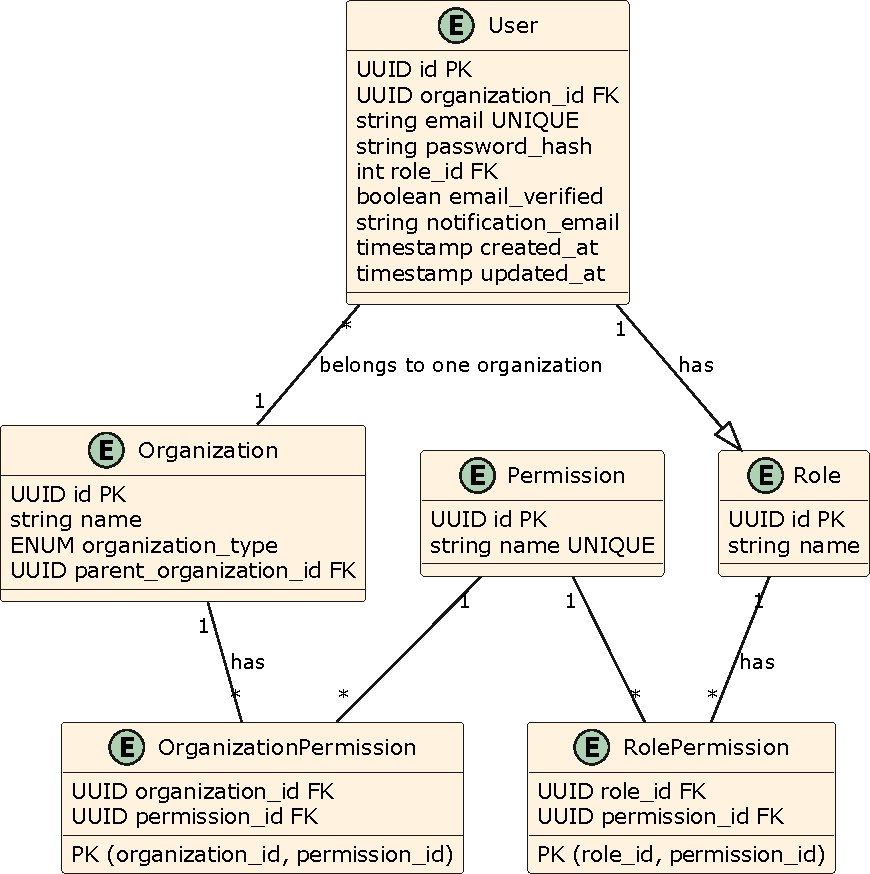
\includegraphics[width=0.5\textwidth]{figures/db-user-organization.pdf}
  \caption{Diagramma ER relativo alla gestione delle organizzazioni, degli utenti e dei permessi.}
  \label{fig:organization-user-permissions}
\end{figure}

\subsubsection{Gestione delle reti e dei profili di protezione}
Il modello di database adotta un approccio basato sui profili, che rappresentano l’unico punto in cui vengono definite le policy di filtraggio. Le reti non contengono direttamente regole di protezione, ma si associano a uno o più profili per determinare quali configurazioni di sicurezza applicare.

\paragraph{Gestione delle reti}
Ogni organizzazione può registrare una o più reti, che rappresentano gli indirizzi IP dai quali provengono le richieste al sistema. Una delle principali innovazioni introdotte in questa modellazione è il supporto alla notazione CIDR, che permette di rappresentare un intero intervallo di indirizzi IP con una sola entry nel database. Questo migliora significativamente l’efficienza del sistema, riducendo il numero di righe necessarie rispetto al modello precedente, in cui ogni indirizzo IP veniva memorizzato singolarmente, anche se appartenente allo stesso range.

Per supportare scenari in cui gli indirizzi IP di una rete cambiano dinamicamente, è presente un meccanismo di aggiornamento tramite \emph{DDNS}. Il database memorizza le informazioni necessarie per gestire queste variazioni, includendo dati di autenticazione e timestamp relativi all’ultimo aggiornamento della rete registrata.

\paragraph{Profili di protezione}
Nel nuovo database, i profili di protezione sono modellati come entità indipendenti, associate a una specifica organizzazione, ma con la possibilità di essere condivise con le organizzazioni a essa subordinate. Questo meccanismo è implementato tramite un attributo che indica se un profilo è ereditabile all'interno della gerarchia. In tal caso, esso risulta visibile e utilizzabile anche per le organizzazioni figlie, evitando la duplicazione delle configurazioni di filtraggio.

\paragraph{Filtri e categorie di protezione}
Ogni profilo può essere associato a una serie di filtri di protezione, che regolano il blocco di contenuti in base a diverse tipologie di criteri. Il sistema prevede una tabella specifica per ciascun tipo di filtro, tra cui:
\begin{itemize}
  \item Blocco per categoria, per contenuto o singolo servizio;
  \item Abilitazione forzata di SafeSearch per i motori di ricerca;
  \item Limitazioni per indirizzi IP e domini.
\end{itemize}

La struttura del database prevede che per ogni opzione bloccata sia presente una riga separata. Ad esempio, se un profilo vieta l’accesso a cinque categorie di contenuti, la tabella relativa al blocco per categorie conterrà cinque righe distinte, ognuna riferita al profilo e alla categoria corrispondente.

Il database consente inoltre di definire i \emph{profili ristretti} attraverso un attributo dedicato, che indica se un profilo opera in modalità restrittiva. In questa configurazione, tutte le protezioni risultano attive di default, mentre l’accesso è consentito esclusivamente ai domini autorizzati. Sebbene l’informazione sia memorizzata nel database, la logica che governa il comportamento di questi profili è demandata al livello applicativo, che interpreta tale configurazione e applica le restrizioni di conseguenza.

\paragraph{Associazione dei profili alle reti}
L’assegnazione di un profilo a una rete avviene attraverso la coppia di server DNS utilizzata per le richieste. Questo meccanismo consente di determinare quale profilo debba essere applicato in base alla configurazione DNS impostata dall’amministratore, evitando così la necessità di separare fisicamente i dispositivi su reti diverse per applicare configurazioni differenti. Nel database, questo concetto è rappresentato dal termine \emph{porta} (\Cref{fig:network-profiles}), una scelta terminologica che potrebbe apparire incoerente rispetto al suo significato tradizionale. Tuttavia, essa deriva da una versione precedente del sistema, in cui la selezione del profilo veniva effettivamente implementata sfruttando il numero della porta TCP.

Questa modellazione permette quindi di gestire scenari avanzati in cui più profili possono coesistere sulla stessa rete, garantendo un elevato livello di flessibilità nella definizione delle policy di filtraggio e riducendo la necessità di configurazioni ridondanti.

\begin{figure}
  \centering
  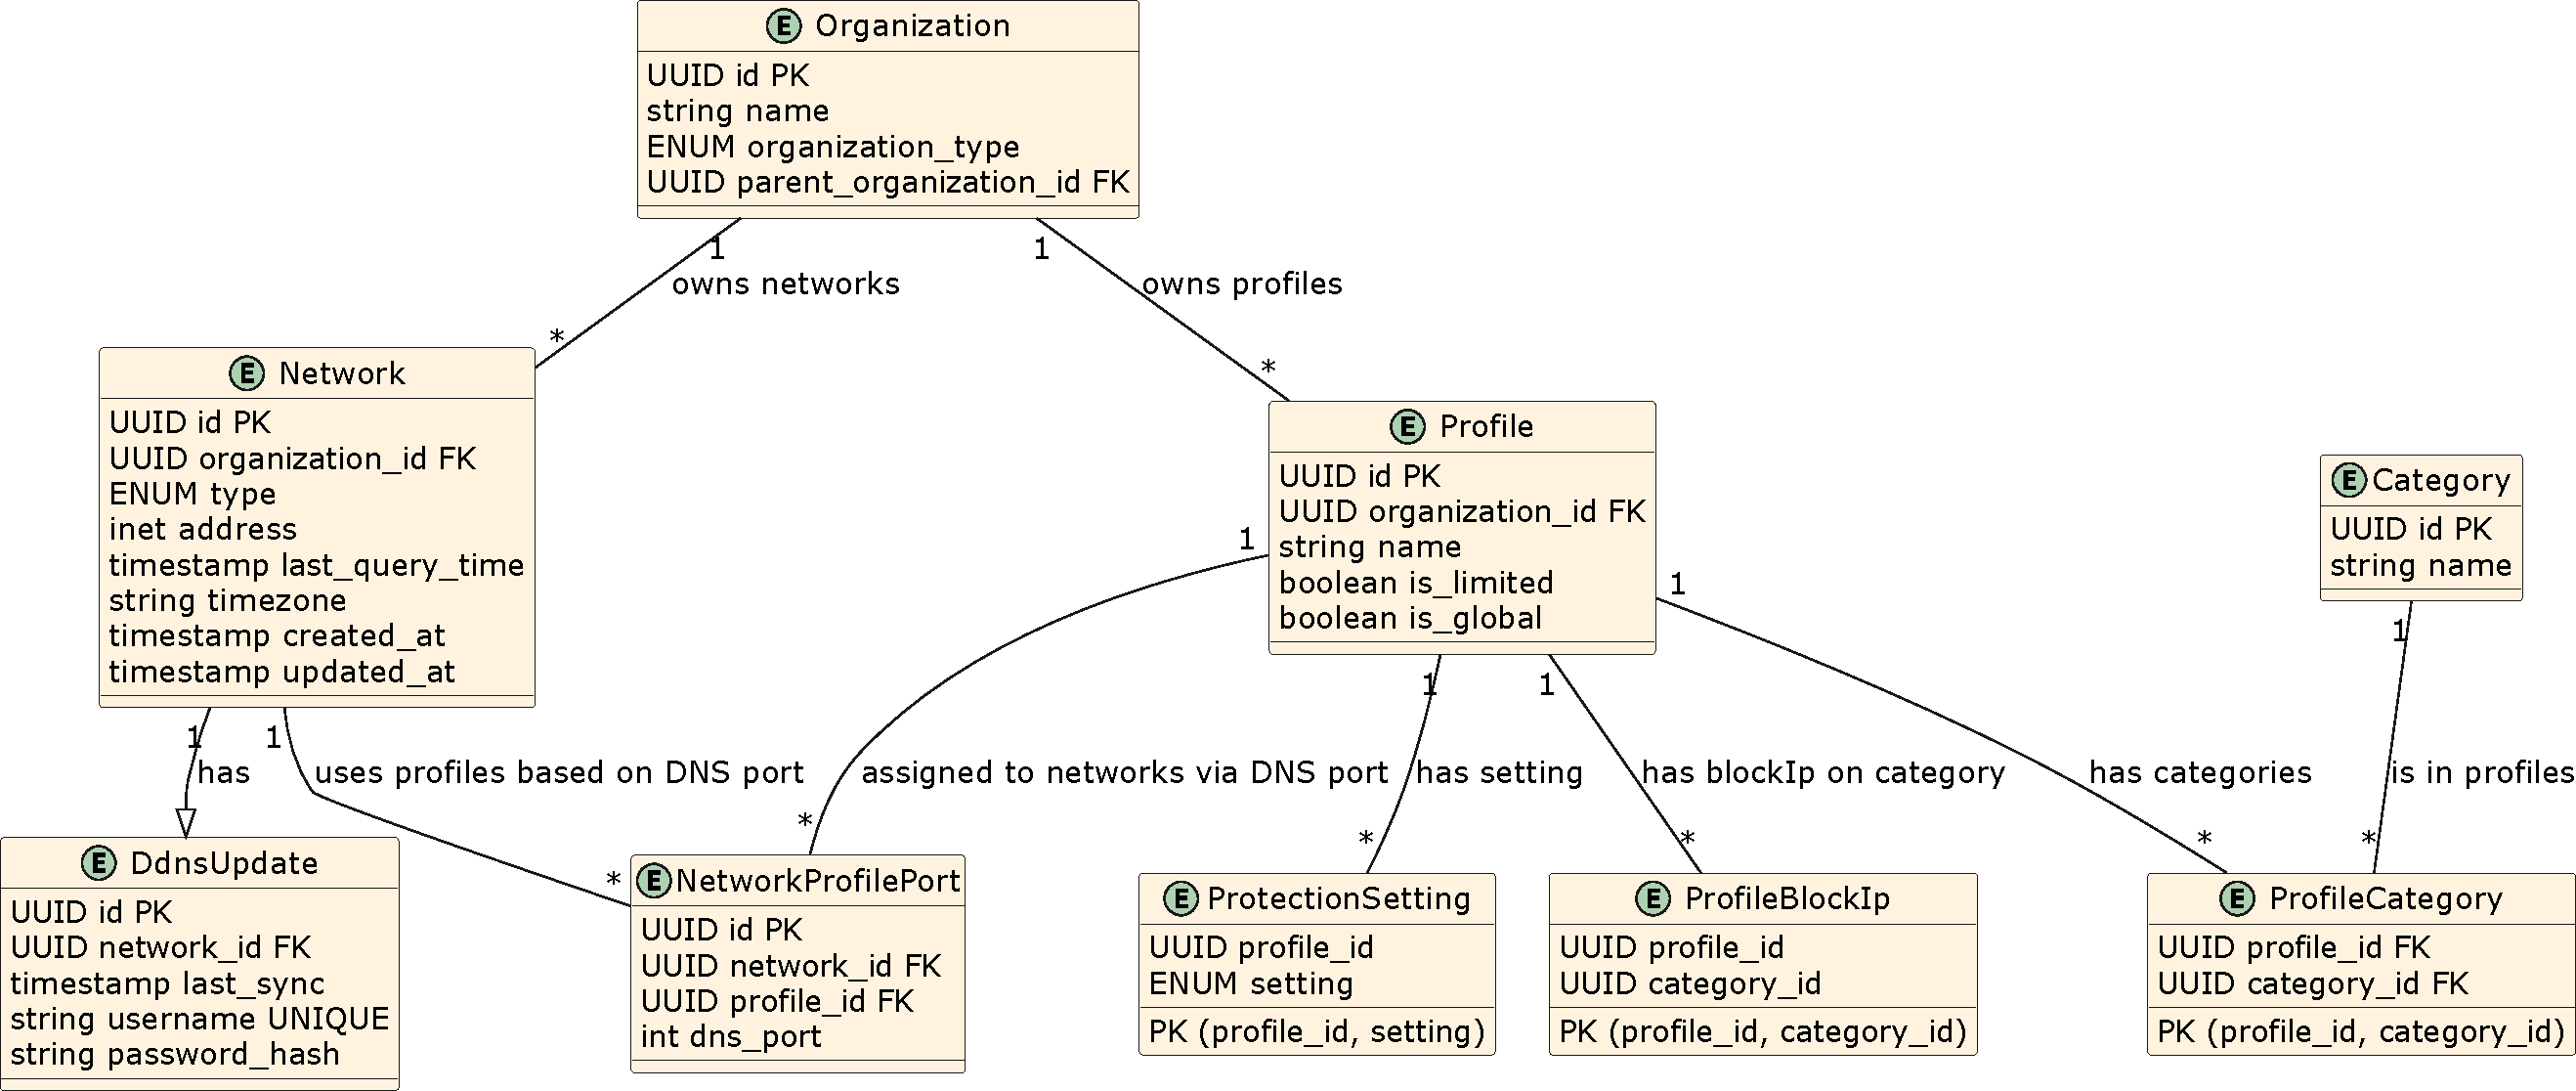
\includegraphics[width=1\textwidth]{figures/db-network-profile.pdf}
  \caption{Diagramma ER relativo alla gestione delle reti e dei profili di protezione.}
  \label{fig:network-profiles}
\end{figure}

\subsubsection{Gestione delle categorie e delle eccezioni}
Il nuovo database introduce una modellazione più strutturata delle categorie di contenuti e delle eccezioni, con l'obiettivo di migliorare la gestione delle configurazioni di filtraggio. Rispetto alla versione precedente, questa modellazione consente una maggiore flessibilità nella definizione delle policy, facilitando sia la gestione delle categorie predefinite sia la creazione di gruppi di eccezioni personalizzati.

\paragraph{Categorie e macrocategorie}
Le categorie rappresentano insiemi di domini classificati in base alla tipologia di contenuti, come \emph{social media}, \emph{streaming}, \emph{contenuti per adulti} e così via. Per migliorare la chiarezza e la gestione delle policy, ogni categoria appartiene a una \emph{macrocategoria}, che raggruppa più categorie affini.

L'introduzione delle macrocategorie non ha solo un valore organizzativo, ma viene sfruttata dal livello applicativo per semplificare le operazioni di configurazione. Grazie a questa struttura, un amministratore può decidere di abilitare o bloccare tutte le categorie appartenenti a una macrocategoria con un'unica azione, senza dover selezionare manualmente ogni singola voce.

\paragraph{Gestione delle categorie nei template}
Il database prevede anche la possibilità di definire insiemi preconfigurati di categorie attraverso il concetto di \emph{Template Category}. Un template di categoria rappresenta una configurazione standardizzata che include molteplici categorie, utile per velocizzare l’applicazione di policy predefinite.
%
L’utilizzo dei template permette di semplificare la gestione delle policy di filtraggio, evitando la necessità di selezionare manualmente ogni singola categoria. Un esempio pratico è la definizione di livelli di protezione preimpostati, con restrizioni progressive, che possono essere selezionati rapidamente senza dover configurare manualmente le singole categorie di contenuti. Questo approccio risulta particolarmente utile per fornire agli utenti meno esperti una modalità intuitiva per applicare politiche di filtraggio senza entrare nel dettaglio delle singole impostazioni.

\paragraph{Gestione avanzata delle eccezioni}
In questo contesto, una delle principali innovazioni rispetto al database precedente riguarda la gestione delle eccezioni. In passato, il sistema si basava esclusivamente su due liste distinte: una per i domini consentiti e una per i domini bloccati. Questo approccio era limitato, poiché ogni profilo doveva gestire separatamente le due liste, senza possibilità di organizzare le eccezioni in modo strutturato.

Il nuovo database introduce il concetto di \emph{gruppi di eccezioni}, che rappresentano insiemi di domini personalizzati contenenti sia elementi bloccati sia consentiti. Ogni gruppo può essere associato a uno o più profili, permettendo così di riutilizzare la stessa configurazione su più contesti senza dover ridefinire manualmente le liste di riferimento. La modellazione delle eccezioni si basa su tre entità principali (\Cref{fig:categories-exceptions}):
\begin{itemize}
  \item \textbf{ExceptionGroup}: rappresenta i gruppi di eccezioni, identificati da un nome.
  \item \textbf{ProfileExceptionGroup}: definisce la relazione tra i profili e i gruppi di eccezioni, consentendo di applicare la stessa configurazione a più profili.
  \item \textbf{DomainExceptionGroup}: stabilisce l'associazione tra i domini e i gruppi di eccezioni, permettendo di definire quali appartengono a un gruppo specifico e se sono bloccati o consentiti.
  \item \textbf{Domain}: rappresenta la lista dei domini inseriti tra le eccezioni.
\end{itemize}

Questa modellazione consente di gestire le eccezioni in modo molto più flessibile, permettendo di definire configurazioni granulari e riutilizzabili. Un’organizzazione può, ad esempio, creare un gruppo di eccezioni che include sia domini consentiti sia domini bloccati e applicarlo a più profili senza dover replicare manualmente le stesse configurazioni. Inoltre, grazie alla presenza dei profili condivisi, anche i gruppi di eccezioni associati a questi ultimi vengono ereditati dalle organizzazioni subordinate. Questo meccanismo consente di mantenere una gestione centralizzata delle eccezioni, assicurando coerenza tra le configurazioni applicate ai diversi livelli della gerarchia organizzativa.

\begin{figure}
  \centering
  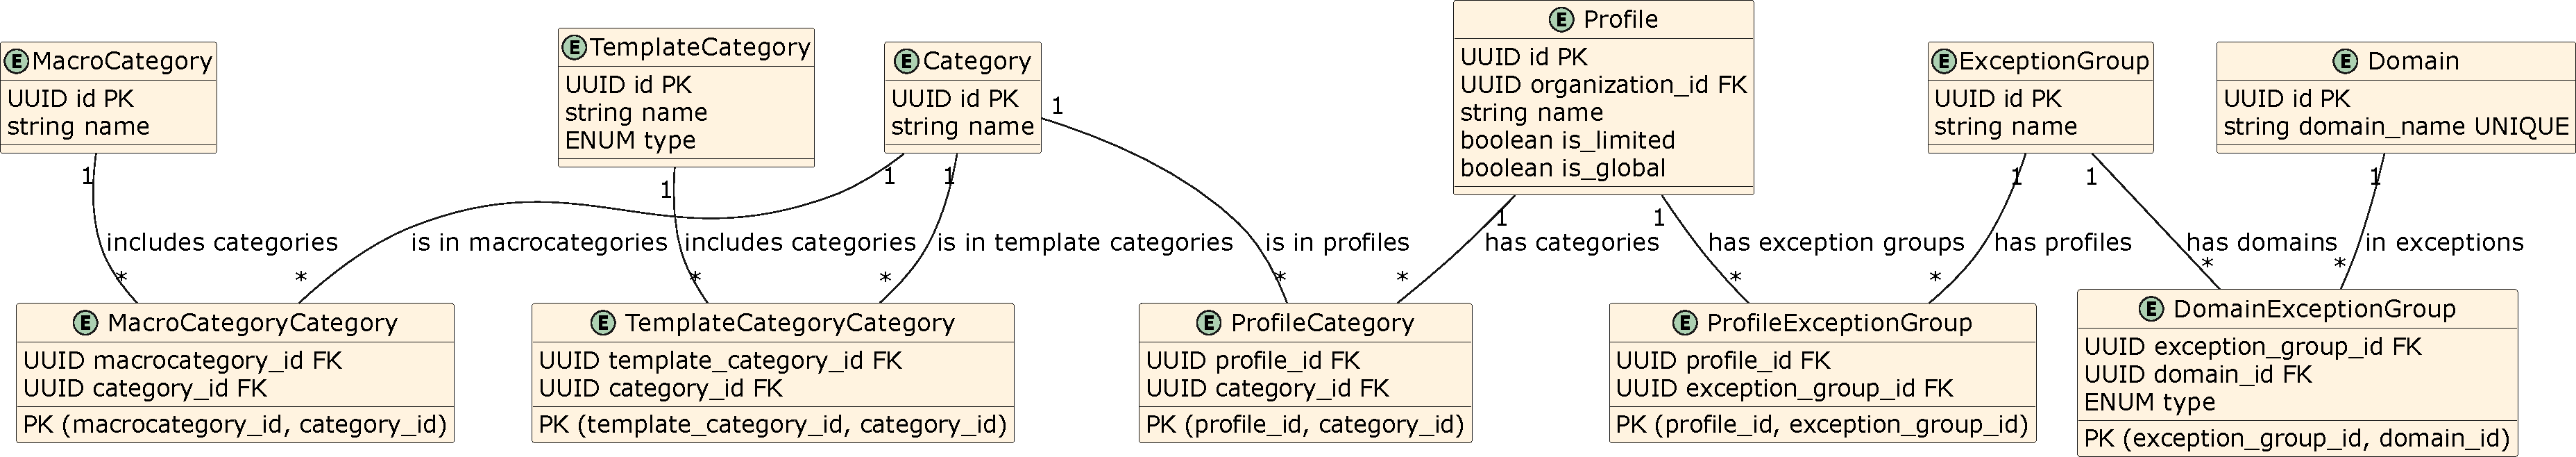
\includegraphics[width=1\textwidth]{figures/db-category-exceptions.pdf}
  \caption{Diagramma ER relativo alla gestione delle categorie e delle eccezioni.}
  \label{fig:categories-exceptions}
\end{figure}

\subsection{Linee guida per la migrazione dei dati}
Il processo di migrazione dei dati rappresenta un'operazione critica nel passaggio dal sistema legacy alla nuova infrastruttura poiché coinvolge informazioni essenziali per il funzionamento del filtro DNS e per l'esperienza degli utenti. Affinché la transizione avvenga in modo efficace, il nuovo sistema dovrà essere già popolato con tutti i dati esistenti prima della sua messa in produzione, evitando così discontinuità operative o perdita di informazioni.

Attualmente, non è ancora stata definita nei dettagli la strategia di migrazione che si vuole adottare, poiché il nuovo sistema si trova in una fase iniziale di sviluppo. Tuttavia, è possibile delineare alcune considerazioni preliminari basate sul confronto tra la struttura del database legacy e la nuova modellazione dei dati. Queste riflessioni costituiscono un primo passo verso la progettazione di un processo di migrazione strutturato, che garantisca coerenza, integrità e compatibilità tra i due ambienti. Di seguito, verranno illustrate alcune linee guida fondamentali per la migrazione, organizzate in base alle principali entità del database. L'obiettivo è fornire un quadro chiaro delle trasformazioni necessarie e delle possibili strategie da adottare per assicurare una transizione fluida e priva di anomalie.

Prima di tutto, un aspetto fondamentale del processo in questione, che coinvolge ogni singola entità da trasferire, riguarda la gestione degli identificativi. Nel vecchio sistema, gli identificativi delle entità erano di natura numerica e seguivano il tipo di dato \texttt{Decimal(1000, 1)} di SQL. Nel nuovo sistema, si utilizzeranno invece identificativi di tipo Universally Unique IDentifier\footnote{\url{https://datatracker.ietf.org/doc/html/rfc9562}} (UUID), garantendo maggiore scalabilità e unicità. Di conseguenza, per ogni entità migrata, sarà necessario generare un nuovo UUID e aggiornare tutte le relazioni di conseguenza. Qualsiasi riferimento all'identificativo legacy dovrà essere tracciato temporaneamente in una tabella di mapping per facilitare il passaggio al nuovo schema.

\subsubsection{Migrazione delle organizzazioni e degli utenti}
La migrazione delle organizzazioni e degli utenti rappresenta un punto cruciale, in quanto bisogna passare da un sistema privo di multiutenza a uno in cui la funzionalità multi-tenant ha guidato lo sviluppo fin dall’inizio. Nel sistema legacy, non esisteva una distinzione tra organizzazione e utente: ogni riga della tabella \texttt{admin} con l'attributo \texttt{tipo = 1} rappresentava sia un cliente che il relativo utente amministratore. Questa struttura era possibile poiché vi era un singolo account per ogni cliente, eliminando la necessità di una separazione tra le due entità.
%
Nel nuovo sistema, invece, utenti e organizzazioni sono stati modellati come entità distinte. La migrazione dovrà quindi adattare i dati esistenti a questa nuova struttura, assicurando che ogni cliente del vecchio database venga convertito in una vera e propria organizzazione, con almeno un utente amministratore associato.

In particolare, il primo passo del processo di migrazione prevede la creazione delle organizzazioni nel nuovo sistema. Ogni riga della tabella \texttt{admin} con \texttt{tipo = 1} dovrà essere trasformata in una entry nella corrispondente tabella del nuovo database. Gli attributi identificativi dell’organizzazione, come il nome, dovranno essere trasferiti e adattati alla nuova struttura.

Per ricreare la gerarchia delle organizzazioni sarà necessario analizzare il valore del campo \texttt{cloud\_idfornitore} della tabella \texttt{admin}. Questo campo, se valorizzato, contiene l’indirizzo email dell’organizzazione padre, ovvero del cliente che gestisce l’entità in questione. Se il campo risulta vuoto, significa che l'organizzazione non è subordinata ad altre ed è quindi posizionata al livello più alto della gerarchia, come nel caso di Dealer o MSP.
%
Nel nuovo sistema, l'associazione tra organizzazioni non avviene più tramite email, ma attraverso l'UUID dell'organizzazione padre. Pertanto, nel processo di migrazione, sarà necessario risolvere queste relazioni traducendo il valore di \texttt{cloud\_idfornitore} nel corrispondente UUID dell'organizzazione padre. Questo passaggio dovrà essere eseguito in due fasi:
\begin{enumerate}
  \item Creare tutte le organizzazioni migrando i dati dalla tabella \texttt{admin}, senza impostare subito il campo \texttt{parent\_organization\_id}.
  \item Dopo che tutte le organizzazioni sono state inserite nel nuovo database, aggiornare il campo \texttt{parent\_organization\_id} associando a ciascuna il corrispondente UUID dell'organizzazione padre, risolvendo la relazione tramite il valore presente in \texttt{cloud\_idfornitore}.
\end{enumerate}
Questa strategia garantisce che la gerarchia venga ricostruita correttamente senza incongruenze nella fase di migrazione.

Successivamente, per ogni organizzazione migrata, dovrà essere creato il corrispondente utente amministratore. Quest'ultimo dovrà essere associato all’organizzazione di riferimento tramite una chiave esterna, garantendo così una chiara relazione tra le due entità. Poiché nel sistema legacy l'utente e l'organizzazione coincidevano, sarà necessario separare logicamente i dati, assicurandosi che il nuovo sistema mantenga coerenza e integrità.

\subsubsection{Migrazione dei profili di protezione}
La migrazione dei profili di protezione rappresenta una delle operazioni più complesse in quanto il nuovo sistema ha introdotto il concetto di profili condivisi, modificando radicalmente la struttura e le modalità di associazione delle configurazioni di filtraggio.

Nel sistema legacy, i profili erano identificati tramite un \textit{codice profilo} e associati ai clienti attraverso la tabella \texttt{admin}, con un legame statico e univoco. Questo significava che ogni profilo apparteneva esclusivamente a un singolo cliente, senza possibilità di essere condiviso tra più entità. Nel nuovo sistema, invece, i profili non sono più legati a una singola istanza del vecchio database, ma vengono associati direttamente alle organizzazioni, con la possibilità di essere riutilizzati dalle organizzazioni subordinate.

Sebbene sia teoricamente possibile effettuare un'analisi per identificare i potenziali profili da trasformare in condivisi, questa operazione risulta particolarmente complessa. Nel database legacy, infatti, non esiste un'informazione chiara e diretta che indichi se un profilo sia utilizzato da più clienti. Questo rende difficile stabilire automaticamente quali profili potrebbero essere condivisi senza introdurre ambiguità o errori nella migrazione.
%
Per garantire una transizione coerente, si può quindi procedere migrando tutti i profili esistenti e impostandoli inizialmente come non condivisibili, riproducendo fedelmente la configurazione che gli utenti avevano nel vecchio pannello. Una volta completata la migrazione, saranno gli stessi amministratori ad avere la possibilità di convertire i profili tradizionali in condivisi e riutilizzarli per più sottoclienti, sfruttando le nuove funzionalità del sistema.

\subsubsection{Migrazione delle categorie di blocco e delle eccezioni}
La migrazione delle categorie di blocco avverrà trasferendo i dati esistenti nelle nuove tabelle, assicurando che le associazioni tra profili e categorie rimangano invariate. Nel sistema legacy, l'associazione tra profilo e categoria era effettuata tramite il codice profilo collegato alla relativa entità nella tabella \texttt{admin}, mentre nel nuovo sistema viene utilizzato l'UUID del profilo. Di conseguenza, la migrazione dovrà prevedere la conversione dei riferimenti al codice profilo nel nuovo identificativo univoco, garantendo la coerenza con la nuova struttura dati.

Un aspetto più critico riguarda la gestione delle eccezioni, che nel nuovo sistema introduce gruppi riutilizzabili anziché liste statiche per ogni profilo. Per garantire una transizione coerente, la migrazione dovrà trasformare le eccezioni esistenti adattandole alla nuova struttura. Una possibile soluzione consiste nel creare un gruppo di eccezioni predefinito per ogni profilo, popolandolo con i domini bloccati e consentiti presenti nel vecchio database. Questo approccio mantiene le configurazioni originali, offrendo al contempo la maggiore flessibilità del nuovo sistema.

\subsubsection{Migrazione delle reti}
La migrazione delle reti richiede un processo di consolidamento degli indirizzi IP per adattarli alla nuova rappresentazione basata sulla notazione CIDR. Anziché memorizzare ogni singolo indirizzo come una entry separata, il nuovo sistema consente di rappresentare un intero range di IP in modo compatto, riducendo la ridondanza e ottimizzando lo spazio di archiviazione.

Per garantire una transizione coerente, la migrazione dovrà prevedere la conversione degli indirizzi IP esistenti nella loro corrispondente rappresentazione CIDR. Questo comporta l’aggregazione degli indirizzi appartenenti allo stesso range e la loro trasformazione in un’unica entry nel nuovo database. Tale processo migliorerà le operazioni di gestione e ricerca delle reti, riducendo significativamente il numero di record memorizzati.

\chapter{Implementazione}

\section{Piano di Sviluppo}
Il processo di sviluppo del nuovo sistema si è basato sulla metodologia \textit{Agile SCRUM}, con cicli di sviluppo iterativi e incrementali della durata di due settimane (\textit{sprint}). Al termine di ogni sprint, si è tenuto un meeting di revisione con il \textit{project manager} (PM), il quale ha supervisionato lo stato di avanzamento del lavoro, analizzato le criticità emerse e verificato la conformità delle ore lavorate rispetto a quelle preventivate. Durante questi incontri, si sono definite le attività per lo sprint successivo, garantendo un flusso di sviluppo costante e ben organizzato.

Il team di sviluppo è composto esclusivamente da \textit{Full Stack Developer}, senza una suddivisione rigida tra frontend e backend. Le attività di progettazione grafica non sono state gestite internamente, ma affidate a un designer esterno, incaricato del rinnovo della brand identity. Quindi, per quanto concerne la UI/UX, il team si è solo ocupato di implementare le nuove interfacce grafiche, seguendo le specifiche fornite dal designer.

Per la gestione e il monitoraggio delle attività, è stato utilizzato lo strumento di project management \textit{ClickUp}\footnote{\url{https://clickup.com/}}, che ha permesso di tracciare i task, assegnare priorità e garantire un'organizzazione efficace del lavoro.

Le attività svolte durante gli sprint hanno incluso lo sviluppo di nuove funzionalità, la risoluzione di bug, il refactoring del codice e l'ottimizzazione delle performance. Particolare attenzione è stata dedicata alla qualità del software, con l'integrazione di test automatici e revisioni periodiche del codice prima del rilascio delle feature.

\subsection{Ambiente di sviluppo e infrastruttura}
L'ambiente di sviluppo è stato configurato in modo da rispecchiare il più possibile l'ambiente di produzione, garantendo una maggiore affidabilità nei test e riducendo il rischio di anomalie legate a differenze infrastrutturali. Per ottenere questa uniformità, sono state adottate tecnologie che permettono di replicare fedelmente la configurazione di produzione.

L'intero sistema di sviluppo è stato containerizzato tramite Docker, con i vari servizi orchestrati tramite Docker Compose. Questo permette di avviare l’ambiente di sviluppo in modo rapido e riproducibile su diverse macchine, riducendo problemi di configurazione tra membri del team. Inoltre, l'uso di \textit{Docker-in-Docker} nella pipeline \textit{CI/CD} consente di replicare l’ambiente di esecuzione anche nei job automatici di test e build.

Per la gestione delle configurazioni, ogni microservizio utilizza un file \texttt{.env}, che contiene le variabili d’ambiente necessarie per la configurazione dinamica dello stesso, come le credenziali di accesso ai database e gli endpoint delle API. Durante l’esecuzione della pipeline CI/CD, questo file viene iniettato nei container, permettendo di mantenere un ambiente coerente tra sviluppo, test e produzione, senza la necessità di configurazioni separate per ciascun contesto.

Per migliorare l'affidabilità dei test, è stata implementata una strategia di \textit{seeding} del database, che consente di popolare l’ambiente di test con dati coerenti ad ogni esecuzione, assicurando risultati riproducibili e verifiche affidabili.

\subsection{Struttura della repository}
L'intero codice del progetto è gestito tramite una \textit{monorepo}, ospitata su GitLab. La scelta di adottare una monorepo è motivata dalla necessità di mantenere in un unico repository sia il frontend che tutti i microservizi che compongono il backend, semplificando la gestione delle dipendenze, la coerenza tra i moduli e l'esecuzione delle pipeline di \textit{Continuous Integration/Continuous Deployment} (CI/CD).

Per ottimizzare la gestione della monorepo, è stato utilizzato \texttt{Turborepo}\footnote{\url{https://turbo.build}}, un tool specificamente progettato per lo sviluppo di applicazioni in TypeScript. Turborepo consente di affrontare in modo efficiente il problema dei lunghi processi di compilazione, tipici delle monorepo con numerosi pacchetti e molteplici task (come compilazione, testing e linting). Il tool pianifica l'esecuzione dei task in modo ottimizzato, parallelizzandoli su tutti i core disponibili e implementando un avanzato sistema di caching. Questo permette di ridurre drasticamente i tempi di build successivi al primo, migliorando la produttività del team di sviluppo.

L'organizzazione della monorepo sfrutta la funzionalità \textit{workspace} di \texttt{pnpm}, suddividendo i pacchetti in due macro-categorie:
\begin{itemize}
  \item \textbf{Apps}: Contiene tutti i servizi che vengono eseguiti in maniera indipendente e che costituiscono i diversi microservizi del sistema. Qui sono presenti il frontend e tutti i componenti del backend che operano come unità autonome.
  \item \textbf{Packages}: Include pacchetti di supporto utilizzati dalle \textit{apps}. Tra questi vi sono il package \texttt{commons}, che contiene definizioni e metodi condivisi tra i vari servizi, i pacchetti dedicati alla gestione dello schema di \textit{Prisma} e all'esportazione del client per il database, oltre ai pacchetti per il seeding di quest'ultimo nella fase di test.
\end{itemize}

\subsubsection{Modello di branching}
Per organizzare al meglio il lavoro di sviluppo del team, è stato adottato un modello di branching strutturato, che consente di gestire in modo chiaro e controllato il ciclo di vita del codice. Esso prevede i seguenti branch principali:
\begin{itemize}
  \item \textbf{Main}: Contiene il codice stabile e rappresenta l'unico branch dal quale si effettuano rilasci in produzione.
  \item \textbf{Unstable}: Include le funzionalità candidate al rilascio in produzione. Il codice qui presente è testato in un ambiente di staging prima di essere eventualmente integrato nel branch \textit{main}.
  \item \textbf{Branch personali}: Ogni sviluppatore lavora principalmente su un branch personale, denominato con il proprio cognome, per eseguire i commit delle proprie modifiche prima di unire il codice nei branch condivisi.
  \item \textbf{Feature branches}: Per lo sviluppo di funzionalità specifiche, possono essere creati branch temporanei, indipendenti dai branch personali, in modo da favorire un'organizzazione più modulare del codice.
\end{itemize}

Questa strategia consente di mantenere un flusso di sviluppo ordinato, con chiara separazione tra il codice in produzione, il codice in fase di test e le modifiche in sviluppo. Inoltre, grazie all'integrazione con le pipeline CI/CD di GitLab, il sistema è in grado di eseguire automaticamente test e build per ogni \textit{push} e \textit{merge request}, garantendo un'elevata affidabilità prima della promozione del codice verso l'ambiente di produzione.

\subsubsection{Pipeline CI/CD}
L'automazione del processo di sviluppo è stata realizzata attraverso una pipeline di \textit{CI/CD}, integrata direttamente in GitLab. La pipeline è suddivisa in più fasi, organizzate per garantire una validazione progressiva del codice prima del rilascio in staging.

L'intero processo di build e test si basa su Docker-in-Docker\footnote{\url{https://www.docker.com/resources/docker-in-docker-containerized-ci-workflows-dockercon-2023}} (DinD), una soluzione che permette alla pipeline di eseguire e gestire container Docker all'interno di ambienti di esecuzione basati sulla stessa tecnologia. Questo approccio consente di costruire immagini Docker direttamente nei job della pipeline, riducendo la dipendenza da infrastrutture esterne e garantendo isolamento ed una maggiore coerenza tra gli ambienti di sviluppo, test e deploy.

Il flusso di lavoro della pipeline prevede le seguenti fasi:
\begin{enumerate}
  \item \textbf{Build dell'ambiente di sviluppo}: I servizi vengono compilati e avviati tramite \texttt{docker-compose}, con supporto alla parallelizzazione dei task e caching per ottimizzare i tempi di build.
  \item \textbf{Esecuzione dei test}: Ogni microservizio è testato in container isolati. Viene eseguito il processo di seeding del database per simulare scenari reali e ottenere una copertura completa del codice.
  \item \textbf{Build per la produzione}: Se i test risultano superati, viene generata una build ottimizzata per il rilascio, con tagging e push delle immagini Docker nel registry di GitLab.
  \item \textbf{Deploy sull'ambiente di staging}: Il codice viene distribuito aggiornando i container in esecuzione e ripristinando il database con i dati necessari per il test pre-produzione.
\end{enumerate}

La pipeline utilizza strategie di caching avanzate per ridurre i tempi di esecuzione. I pacchetti \texttt{pnpm} e la cache di \texttt{Turborepo} vengono riutilizzati tra i job, evitando ricompilazioni non necessarie. Inoltre, il sistema di \textit{retry} assicura la ripetizione automatica dei job in caso di errori transitori, migliorando l'affidabilità del processo.

Grazie a questa configurazione della pipeline è possibile garantire un flusso di sviluppo strutturato e sicuro, assicurando che solo codice stabile e testato venga promosso verso l'ambiente di staging e, successivamente, alla produzione.

\subsection{Test e controllo qualità}
Una componente fondamentale del piano di sviluppo è stata la verifica della qualità del codice e la sua copertura tramite test automatizzati. Il processo di testing ha seguito le seguenti linee guida:
\begin{itemize}
  \item \textbf{Copertura al 100\%} del codice backend e frontend tramite test unitari e di integrazione.
  \item Per i test lato backend è stata utilizzata la libreria \texttt{Mocha}\footnote{\url{https://mochajs.org}}, che permette di eseguire test unitari e di integrazione in un ambiente controllato, verificando il corretto funzionamento delle API e della logica applicativa.
  \item Per quelli lato frontend è stato invece adottato \texttt{Playwright}\footnote{\url{https://playwright.dev}}, uno strumento per il testing end-to-end che consente di simulare interazioni utente su più browser. Tuttavia, la copertura dei test frontend è ancora da ampliare per garantire una validazione più completa dell'interfaccia utente.
  \item Utilizzo di strumenti di analisi statica del codice come \texttt{ESLint}\footnote{\url{https://eslint.org}} e \texttt{Prettier}\footnote{\url{https://prettier.io}} per garantire standard di qualità e uniformità nella formattazione.
  \item Verifica delle performance e dei comportamenti critici del sistema mediante test prestazionali.
\end{itemize}

\subsection{Approccio alla reingegnerizzazione}
Come descritto nella \Cref{sec:reingegnerizzazione-approcci-fasi}, ogni modello di reingegnerizzazione presenta vantaggi e criticità differenti. Il processo adottato in questo contesto si pone a metà tra l'approccio ``Big Bang'' e quello ``Evolutivo''. Lo sviluppo del nuovo sistema è già avviato e procede in modo incrementale, senza tuttavia una fase di coesistenza con il vecchio. Una volta completato, esso sostituirà integralmente il sistema precedente, fatta eccezione per alcune funzionalità che continueranno a essere gestite dal legacy senza necessità di retrocompatibilità.

La transizione avverrà in modo diretto, senza un rilascio graduale in produzione. Questo semplifica la migrazione, evitando la necessità di interfacce di compatibilità tra i due sistemi. Tuttavia, a differenza di un classico approccio ``Big Bang'', lo sviluppo non è stato affrontato come una riscrittura monolitica. Il nuovo sistema, infatti, è stato progettato fin dall'inizio con un'architettura a microservizi, organizzata sulla base delle funzionalità piuttosto che sulla replica della struttura esistente.

Questo approccio ibrido permette di bilanciare i vantaggi dei due modelli. La sostituzione completa del vecchio sistema eliminerà la necessità di mantenere allineate due versioni in parallelo, riducendo la complessità operativa. Allo stesso tempo, l'architettura modulare migliorerà la manutenibilità e faciliterà l'integrazione di nuove tecnologie nel tempo. Questa fusione di metodologie garantirà una transizione più controllata, riducendo il rischio di regressioni e assicurando una maggiore stabilità per il sistema finale.

\section{Implementazione della gestione degli errori}
La gestione degli errori rappresenta un aspetto cruciale dell’implementazione del nuovo sistema, garantendo uniformità e coerenza tra backend e frontend. Come descritto nella \Cref{sec:error-management} del capitolo precedente, il design della gestione degli errori è stato strutturato attorno a un modello tipizzato e scalabile, che consente di categorizzare le anomalie in base alla loro natura e al contesto in cui si verificano. In questa sezione verrà illustrata l'implementazione di questo modello, partendo dalla struttura del backend e analizzando successivamente il meccanismo di gestione degli errori nel frontend

\subsection{Gestione degli errori nel backend}
Nel backend, la gestione degli errori è stata implementata attraverso una struttura tipizzata e centralizzata, che garantisce una rappresentazione coerente delle anomalie e facilita la comunicazione con il frontend. Il sistema si basa su una gerarchia di classi che categorizzano le diverse tipologie di errore, sfruttando appieno il sistema di tipi di TypeScript per garantire sicurezza e scalabilità. In questa sezione si analizzeranno nel dettaglio le componenti principali dell’implementazione, tra cui la classe base \texttt{AppError}, il tipo \texttt{AppErrorPayload} e il meccanismo di mappatura degli errori tramite \texttt{ErrorDetailsMapping}.

\subsubsection{Struttura di \texttt{ErrorDetailsMapping}}
Un elemento cardine nella gestione degli errori in questo contesto è la struttura \texttt{ErrorDetailsMapping}, che definisce un sistema di mappatura tra i codici d'errore e le informazioni aggiuntive associate a ciascuno di essi. Questa mappatura consente di tipizzare in modo rigoroso le eccezioni all'interno del sistema, garantendo coerenza tra backend e frontend.

Il tipo \texttt{ErrorDetailsMapping} è stato implementato utilizzando il concetto di \textit{Discriminated union} \footnote{\url{https://www.typescriptlang.org/docs/handbook/2/narrowing.html\#discriminated-unions}}, una tecnica avanzata di TypeScript che permette di creare un'unione di tipi distinti, ciascuno caratterizzato da un identificatore univoco. Questo approccio consente di associare a ogni codice d'errore una specifica struttura dati, evitando il rischio di assegnare dettagli incoerenti o incompleti a una determinata tipologia di errore.

Di seguito è riportata una porzione della definizione di \texttt{ErrorDetailsMapping}:

\lstinputlisting[
  language=typescript,
  caption={Porzione di \texttt{ErrorDetailsMapping}},
label={lst:errorDetailsMapping}]{listings/errorDetails.ts}

La mappatura è organizzata in diverse categorie di errori, ciascuna caratterizzata da una stringa identificativa che segue una convenzione specifica. Ad esempio, gli errori relativi alla validazione degli input sono contrassegnati dal prefisso ``\texttt{validation}'', mentre quelli legati alla gestione delle entità utente utilizzano prefissi come ``\texttt{user}''. Questo schema permette di mantenere un'organizzazione chiara e prevedibile all'interno del codice. Da notare che questi prefissi sono stati scelti in modo da rispecchiare la struttura delle cartelle che usa il frontend per organizzare i file relativi alle traduzioni di tutte le strinche di testo presenti nell'applicazione.

Ogni chiave di \texttt{ErrorDetailsMapping} è associata a un oggetto che definisce i dettagli dell’errore corrispondente. Ad esempio, il codice ``\texttt{user.not\_found}'' è mappato su un oggetto che contiene un solo campo, \texttt{userId}, il quale rappresenta l'identificativo dell'utente che non è stato trovato. Al contrario, errori più complessi, come quelli relativi alla creazione di un utente, includono un campo \texttt{cause} che specifica la motivazione dell'errore. Tale campo è stato anch'esso definito come tipo, sfruttando gli \textit{Union Types}\footnote{\url{https://www.typescriptlang.org/docs/handbook/2/everyday-types.html\#union-types}} di TypeScript su tipi letterali.

Per rendere la gestione degli errori più espressiva e facilmente interpretabile, la definizione dei dettagli di alcuni errori si basa su una gerarchia di tipi, che sfrutta le unioni di stringhe per categorizzare le cause in modo strutturato. Ad esempio, nel caso di un errore durante la creazione di un'entità, la causa può essere una violazione di unicità o un problema di vincolo di chiave esterna nel database. La seguente definizione mostra come tali categorie di errore siano tipizzate:

\lstinputlisting[language=typescript, caption={Definizione del tipo \texttt{cause} per operazioni di creazione}, label={lst:createErrorCause}]{listings/errorTypes.ts}

Questa strategia permette di mantenere un elevato livello di tipizzazione e controllo statico sugli errori generati dal backend. Ogni valore di \texttt{CreateErrorCause} è riconducibile a una stringa specifica che rappresenta la causa esatta dell'errore, evitando di dover gestire messaggi arbitrari e favorendo una comunicazione chiara tra backend e frontend.

Un ulteriore vantaggio di questa struttura è la sua leggibilità. I codici di errore e le relative cause sono stati definiti in modo schematico per essere facilmente convertibili in una stringa leggibile da un umano, permettendo così al frontend di tradurli in messaggi comprensibili per l'utente finale. Questo meccanismo consente di centralizzare la gestione delle stringhe di errore senza doverle definire manualmente nel backend, migliorando la manutenibilità e la scalabilità del sistema.

L'utilizzo di una \textit{Discriminated Union} in questo contesto è particolarmente vantaggioso perché consente di sfruttare il controllo statico dei tipi offerto da TypeScript. In particolare, questa struttura garantisce che:
\begin{itemize}
  \item Ogni codice d’errore sia sempre associato ai dati corretti, evitando ambiguità nella gestione delle eccezioni.
  \item Il frontend possa interpretare correttamente le informazioni restituite dal backend senza necessità di controlli manuali sul tipo dei dati.
  \item L’aggiunta di nuove tipologie di errore sia semplice e non impatti le funzionalità esistenti, rendendo il sistema facilmente estendibile.
\end{itemize}

In sintesi, la struttura \texttt{ErrorDetailsMapping} rappresenta il punto di riferimento per la gestione tipizzata degli errori nel sistema, fornendo un modello scalabile, sicuro e coerente per il trattamento delle anomalie.

\subsubsection{Classe \texttt{AppError}}
La gestione degli errori nel backend si basa anche su una classe astratta denominata \texttt{AppError}, che funge da base per la definizione di tutte le eccezioni applicative. Questa classe fornisce un modello coerente per la rappresentazione degli errori, assicurando che ogni anomalia venga espressa attraverso un formato strutturato e facilmente interpretabile dal sistema. L'obiettivo principale è quello di centralizzare la gestione degli errori, evitando soluzioni dispersive e garantendo una chiara separazione tra la logica applicativa e il trattamento delle anomalie.

Per garantire la massima flessibilità e sicurezza dei tipi, la classe \texttt{AppError} sfrutta i \textit{Generics}\footnote{\url{https://www.typescriptlang.org/docs/handbook/2/generics.html}} di TypeScript. Questo approccio consente di vincolare ogni istanza di errore a un preciso codice identificativo, associandolo a un insieme di dettagli specifici definiti nel tipo \texttt{ErrorDetailsMapping}. Grazie a questa struttura, ogni errore è caratterizzato da tre elementi principali: un codice univoco, uno stato HTTP corrispondente e un set di dettagli contestuali che forniscono informazioni aggiuntive sull'errore.

\lstinputlisting[language=TypeScript,label={lst:appError},caption={Implementazione della classe \texttt{AppError}}]{listings/appError.ts}

\paragraph{Definizione del tipo generico per \texttt{AppError}}
Un elemento fondamentale dell'implementazione della classe \texttt{AppError} è l'uso della keyword \texttt{keyof}\footnote{\url{https://www.typescriptlang.org/docs/handbook/2/keyof-types.html}} durante la definizione del tipo generico \texttt{K}. Questo costrutto di TypeScript, visionabile a riga 2 del \Cref{lst:appError}, consente di ottenere un'unione di stringhe che rappresentano tutti i possibili codici d'errore previsti nel sistema. In altre parole, \texttt{keyof ErrorDetailsMapping} genera dinamicamente un insieme di stringhe che corrispondono esattamente ai nomi delle chiavi definite in \texttt{ErrorDetailsMapping}.
%
Consideriamo, ad esempio, la seguente struttura tipizzata di errori:
\begin{lstlisting}[language=typescript, caption={Esempio di unione di stringhe generate da \texttt{keyof}}]
  "validation.input_error" | "internal.database_error" | "user.create_failed"
\end{lstlisting}
%
Grazie a questo meccanismo, il parametro generico \texttt{K} della classe \texttt{AppError} è automaticamente limitato ai valori validi definiti in \texttt{ErrorDetailsMapping}. In questo modo, qualsiasi istanza della classe d'errore può essere creata solo con un codice conforme alle specifiche del sistema, evitando l'utilizzo di stringhe arbitrarie che potrebbero causare errori di inconsistenza.

\paragraph{Vincolo sul tipo dei dettagli dell’errore}
Oltre a garantire che il codice di errore appartenga a un insieme predefinito, il tipo generico \texttt{K} consente anche di vincolare il formato dei dettagli associati all’errore. Ogni codice d’errore definito in \texttt{ErrorDetailsMapping} è associato a un oggetto contenente informazioni specifiche per quel particolare tipo di anomalia. La classe \texttt{AppError} assicura che il campo \texttt{details} rispetti esattamente la struttura prevista per il codice d’errore selezionato.
%
Ad esempio, se si crea un'istanza di errore per rappresentare un utente non trovato, TypeScript garantirà che i dettagli contengano esclusivamente le proprietà previste per quel tipo di errore. Il codice nel \Cref{lst:appErrorUsage} mostra un caso d’uso concreto:

\lstinputlisting[language=typescript, caption={Esempio di utilizzo della classe \texttt{AppError}}, label={lst:appErrorUsage}]{listings/appErrorUsage.ts}
%
In questo caso, il codice dell'errore è limitato alla stringa ``\texttt{user.not\_found}'', e i dettagli sono strutturati esattamente come specificato in \texttt{ErrorDetailsMapping}. Se si tentasse di fornire un oggetto dettagli con proprietà non conformi, TypeScript genererebbe un errore a tempo di compilazione, impedendo di introdurre inconsistenze nel sistema.

Questa strategia, combinata con il sistema di tipi di TypeScript, permette di mantenere una gestione degli errori robusta, sicura e facilmente estendibile. Nuovi codici d’errore possono essere aggiunti semplicemente aggiornando \texttt{ErrorDetailsMapping}, senza dover modificare la logica esistente o introdurre controlli manuali.

\paragraph{Definizione del tipo \texttt{AppErrorPayload}}
Un altro elemento centrale di \texttt{AppError} è il metodo \texttt{toJSON()}, il quale ha il compito di serializzare l’errore in un formato compatibile con la comunicazione tra backend e frontend. Questo metodo restituisce un oggetto che segue la struttura imposta dal tipo \texttt{AppErrorPayload}, definito nel \Cref{lst:appErrorPayload}.

\newpage
\lstinputlisting[language=typescript, caption={Definizione del tipo \texttt{AppErrorPayload}}, label={lst:appErrorPayload}]{listings/appErrorPayload.ts}
La sintassi utilizzata in questa definizione sfrutta alcune funzionalità avanzate di TypeScript:
\begin{itemize}
  \item \textbf{Mapped Types}: La parte di codice a linea 2 itera su ciascuna chiave \texttt{K} presente in \texttt{ErrorDetailsMapping}. Per ogni chiave, viene creato un nuovo tipo \textit{object} avente due proprietà:
    \begin{itemize}
      \item \texttt{code} di tipo \texttt{K}, che rappresenta il codice d’errore,
      \item \texttt{details} di tipo \texttt{ErrorDetailsMapping[K]}, che contiene i dettagli specifici associati a quel codice.
    \end{itemize}

  \item \textbf{Indexed Access Types}: L'intera mappatura è poi indicizzata con \texttt{[keyof ErrorDetailsMapping]} a linea 6. Questa operazione estrae, dall'oggetto mappato, una unione di tutti i tipi generati per ogni chiave. In altre parole, il risultato finale è una unione dei tipi object definiti per ciascuna chiave in \texttt{ErrorDetailsMapping}.
\end{itemize}

In sintesi, \texttt{AppErrorPayload} rappresenta uno union type, in cui ogni membro dell'unione è un oggetto con due proprietà:
\begin{itemize}
  \item \texttt{code}, il quale contiene un identificativo dell'errore,
  \item \texttt{details}, il quale fornisce informazioni specifiche associate a quell'errore, basate sulla mappatura definita in \texttt{ErrorDetailsMapping}.
\end{itemize}

Questo design consente a \texttt{AppError} di gestire in modo robusto e tipizzato una serie di errori diversi, garantendo che ogni di essi abbia una struttura dati coerente e ben definita.

\chapter{Valutazione}

L'obiettivo del presente capitolo è discutere i risultati finora ottenuti, in particolare sulla base dei requisiti già soddisfatti e delle migliorie introdotte dal nuovo sistema rispetto alla versione legacy. Poiché il sistema è ancora in fase di sviluppo, non è possibile fornire una valutazione complessiva, effettuare un confronto esaustivo con il vecchio sistema, né presentare risultati di test prestazionali e di usabilità. Tuttavia, è possibile analizzare le funzionalità già progettate e implementate, valutandone il contributo rispetto agli obiettivi iniziali e identificando le garanzie che il nuovo sistema è già in grado di fornire.

\section{Requisiti soddisfatti}
Sin dall'inizio era stato stabilito che questa tesi non avrebbe condotto alla realizzazione completa del sistema, ma si sarebbe concentrata principalmente sulle fondamentali fasi di analisi e progettazione, includendo anche l'implementazione di una prima versione funzionale. Nonostante ciò, è possibile tracciare un bilancio dei requisiti già soddisfatti, i quali evidenziano le potenzialità del nuovo sistema rispetto al precedente. A tal fine, i requisiti verranno suddivisi in due categorie: quelli già soddisfatti sia dal punto di vista progettuale che implementativo e quelli attualmente soddisfatti solo dal punto di vista progettuale.

\subsection{Elementi progettati e implementati}
Tra i requisiti soddisfatti, alcuni non si limitano alla fase di progettazione ma sono già stati concretamente implementati, costituendo il nucleo della prima versione del sistema. Questi elementi forniscono un primo miglioramento rispetto al legacy e rappresentano una base solida per l’evoluzione futura del progetto. Di seguito vengono analizzate le funzionalità già operative, evidenziandone l'impatto e le garanzie offerte.

\subsubsection{Dashboard panoramica per MSP e Dealer}
La prima funzionalità significativa già implementata è la dashboard panoramica, progettata specificamente per MSP e Dealer. Nel sistema legacy, questi utenti non disponevano di una visione aggregata ed efficace dei clienti sotto la loro gestione. Il nuovo sistema, invece, include una schermata con statistiche e grafici che permettono di ottenere una panoramica dettagliata delle attività del filtro DNS. In particolare, la dashboard mostra le seguenti informazioni:

\begin{itemize}
  \item Nella parte superiore, vengono presentate statistiche di base relative alle richieste elaborate dal filtro. Tra queste: il numero totale di richieste ricevute, il numero di minacce bloccate, il numero di categorie e indirizzi IP bloccati, il numero di categorie consentite, il numero di richieste DNS non risolte (NXDOMAIN) e, infine, il numero di richieste che hanno forzato l’utilizzo della SafeSearch sui motori di ricerca e YouTube. Questi dati offrono un quadro generale sul funzionamento del sistema e sull'efficacia del filtraggio.

  \item Nella parte centrale, sono presenti grafici per monitorare l’andamento delle richieste DNS. In particolare, vi è:
    \begin{itemize}
      \item Un grafico a barre che mostra le cinque categorie più bloccate;
      \item Un grafico a torta che rappresenta la distribuzione percentuale delle richieste DNS in base alla loro tipologia (richieste bloccate, richieste consentite, blocchi per IP, domini non risolti).
    \end{itemize}

  \item Nella parte inferiore, è presente un grafico che mostra l’andamento delle richieste DNS nel tempo, distinguendo tra quelle bloccate e quelle consentite.

  \item Tutti e tre i grafici consentono di modificare l'intervallo temporale di visualizzazione, permettendo di analizzare i dati su finestre temporali di 24, 48 o 72 ore.
\end{itemize}
%
Oltre a offrire una panoramica complessiva, la dashboard consente di visualizzare statistiche e report specifici per ciascun cliente gestito dall’MSP o dal Dealer. È infatti possibile selezionare un cliente dall'apposito menu a tendina e ottenere un quadro dettagliato delle sue attività. Questa funzionalità risulta particolarmente utile per monitorare eventuali anomalie o problemi specifici di un singolo cliente.

Al momento, la dashboard è ancora in una fase iniziale e non è possibile esprimere garanzie sulla qualità dell'aggregazione dei dati, che verrà affinata con le iterazioni successive dello sviluppo.

\begin{figure}
  \centering
  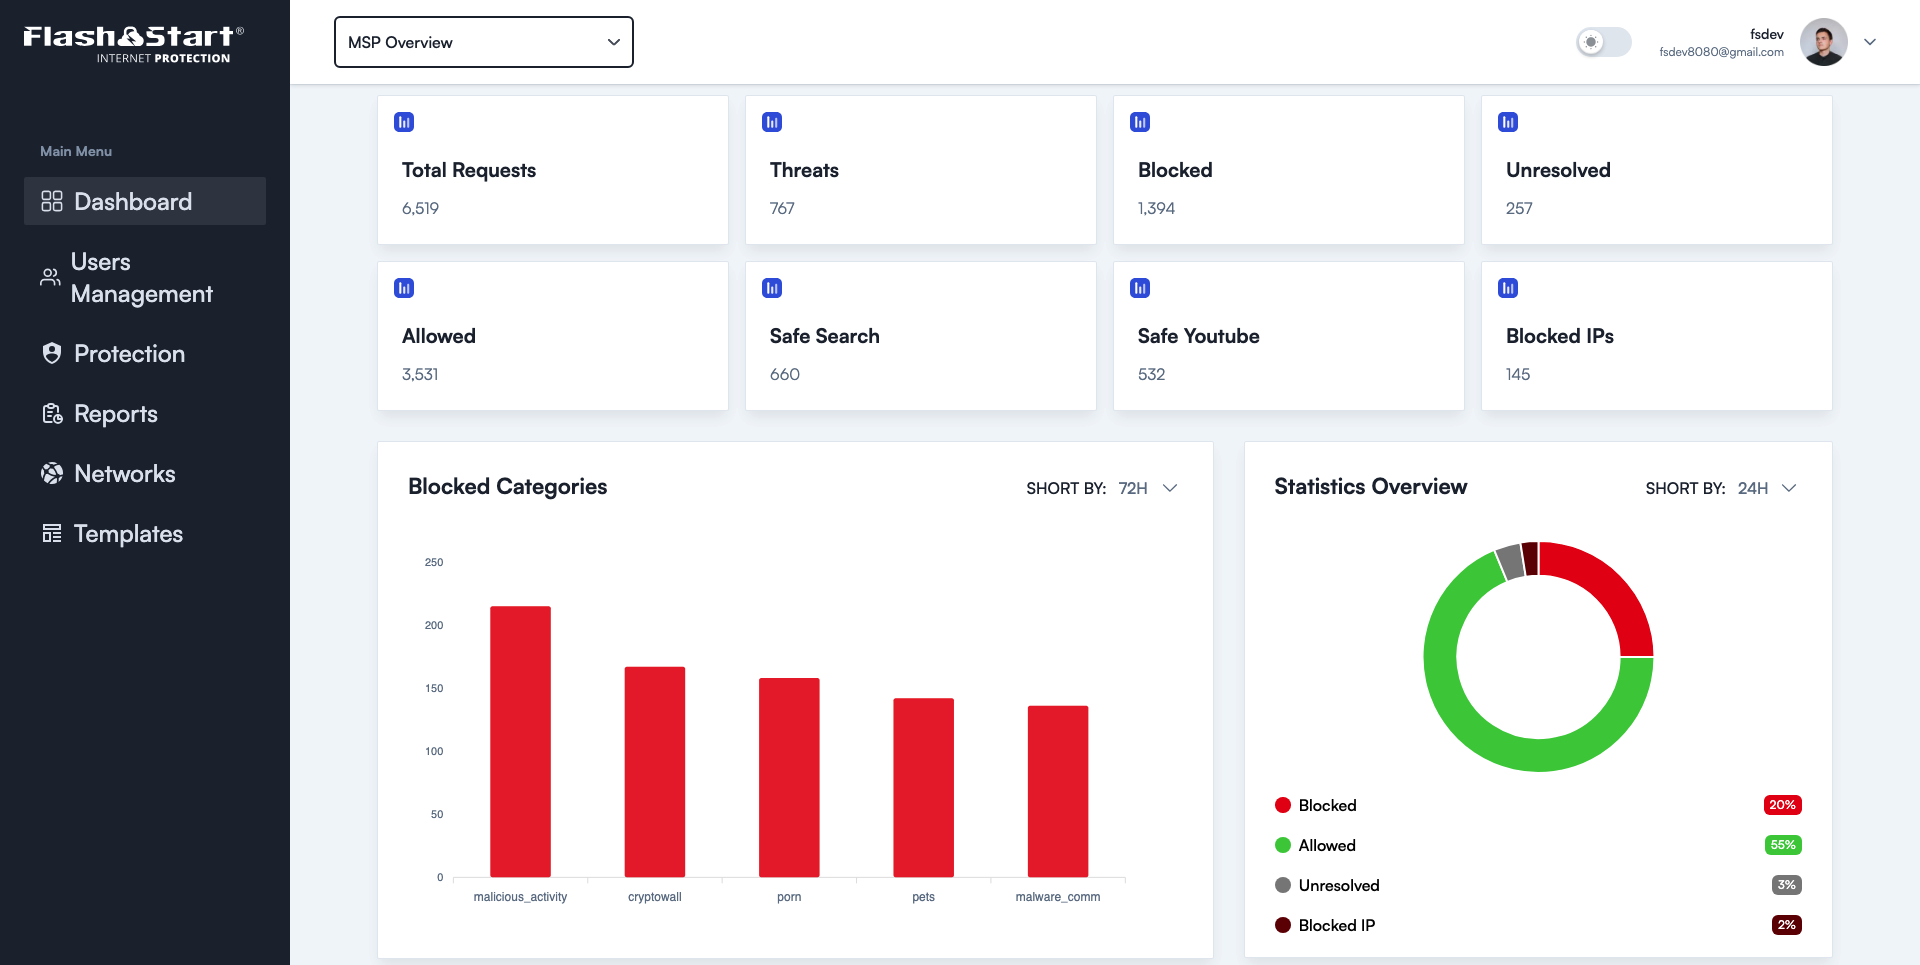
\includegraphics[width=1\textwidth]{figures/new-dashboard.png}
  \caption{Schermata del nuovo sistema che rappresenta la dashboard MSP.}
  \label{fig:dashboard-msp}
\end{figure}

\paragraph{Struttura e layout della dashboard}
Dal punto di vista dell’interfaccia utente, come si può vedere in \Cref{fig:dashboard-msp}, la dashboard è stata progettata con una struttura chiara e organizzata per garantire un’esperienza di navigazione fluida. Il menu di navigazione, posizionato nella parte sinistra dello schermo, è sempre visibile indipendentemente dalla pagina in cui ci si trova. Nei dispositivi aventi un display ridotto, come gli smartphone, il menu rimane nascosto per ottimizzare lo spazio e può essere aperto su richiesta dall’utente.

Nella parte superiore dell’interfaccia sono presenti diversi elementi chiave:
\begin{itemize}
  \item \textbf{Il logo dell'azienda}, posizionato a sinistra.
  \item \textbf{Il selettore del cliente}, che consente agli MSP di filtrare i report per un cliente specifico, oppure di lasciare l’opzione predefinita per visualizzare la panoramica di tutti i clienti gestiti.
  \item \textbf{Il selettore del tema}, situato sulla destra, che permette di passare dalla modalità scura a quella chiara.
  \item \textbf{L’area utente autenticato}, da cui è possibile accedere alle impostazioni del profilo e alla funzione di logout.
\end{itemize}
%
In futuro, nell’header verrà integrata una sezione notifiche, accessibile tramite un’icona che indicherà la presenza di nuovi avvisi e permetterà di visualizzarli all’interno di un pannello dedicato.

Infine, il corpo centrale della dashboard ospita i grafici e le statistiche descritte in precedenza, fornendo un’analisi dettagliata del traffico DNS e della sicurezza del sistema. L’interfaccia è stata progettata per garantire flessibilità, con un layout adattivo che ottimizza la visualizzazione su schermi di diverse dimensioni.

\subsubsection{Gestione della multiutenza}
La necessità di introdurre un sistema che supportasse la multiutenza ha costituito uno dei principali requisiti per il nuovo pannello. Rispetto al precedente, in cui la gestione degli account risultava assai limitata, la nuova implementazione permette ora di associare più credenziali di accesso a una singola organizzazione e di abilitare operazioni di creazione, modifica ed eliminazione degli utenti. Questa flessibilità si traduce in un notevole progresso rispetto al passato, consentendo a più persone, con diversi ruoli, di accedere alla dashboard e monitorare le informazioni di loro competenza.

Un ulteriore aspetto riguarda la futura integrazione del controllo degli accessi: sebbene tale meccanismo non sia ancora stato sviluppato, l’architettura del sistema è stata progettata per accogliere in modo agevole e graduale soluzioni di autorizzazione avanzate, basate su ruoli e permessi granulari. In questo modo, sarà possibile estendere ulteriormente la sicurezza e la modularità del pannello.

Sul fronte della protezione delle credenziali di accesso, è stato adottato l’algoritmo di hashing \texttt{bcrypt}. Quest’ultimo offre non solo una maggiore sicurezza contro attacchi di forza bruta, ma consente anche di aumentare il costo computazionale dell’hashing nel tempo, adeguandone la resistenza alla continua crescita della potenza di calcolo. In questo modo, il sistema può mantenere un elevato livello di protezione delle password anche sul lungo termine.

Per consentire una gestione semplice e immediata della multiutenza, è stata sviluppata un’apposita interfaccia che permette di inserire, aggiornare o rimuovere gli account, oltre che di assegnare a ogni utente un ruolo specifico all’interno dell’organizzazione. Tale funzionalità costituisce le fondamenta su cui verrà costruito in futuro un sistema di controllo degli accessi più sofisticato, in grado di differenziare i privilegi sulle singole risorse applicative.

Nella \Cref{fig:user-management} viene mostrata la schermata dedicata alla gestione degli utenti, in cui è possibile osservare le form per l’inserimento, la modifica e l’eliminazione degli account.

\begin{figure}
  \centering
  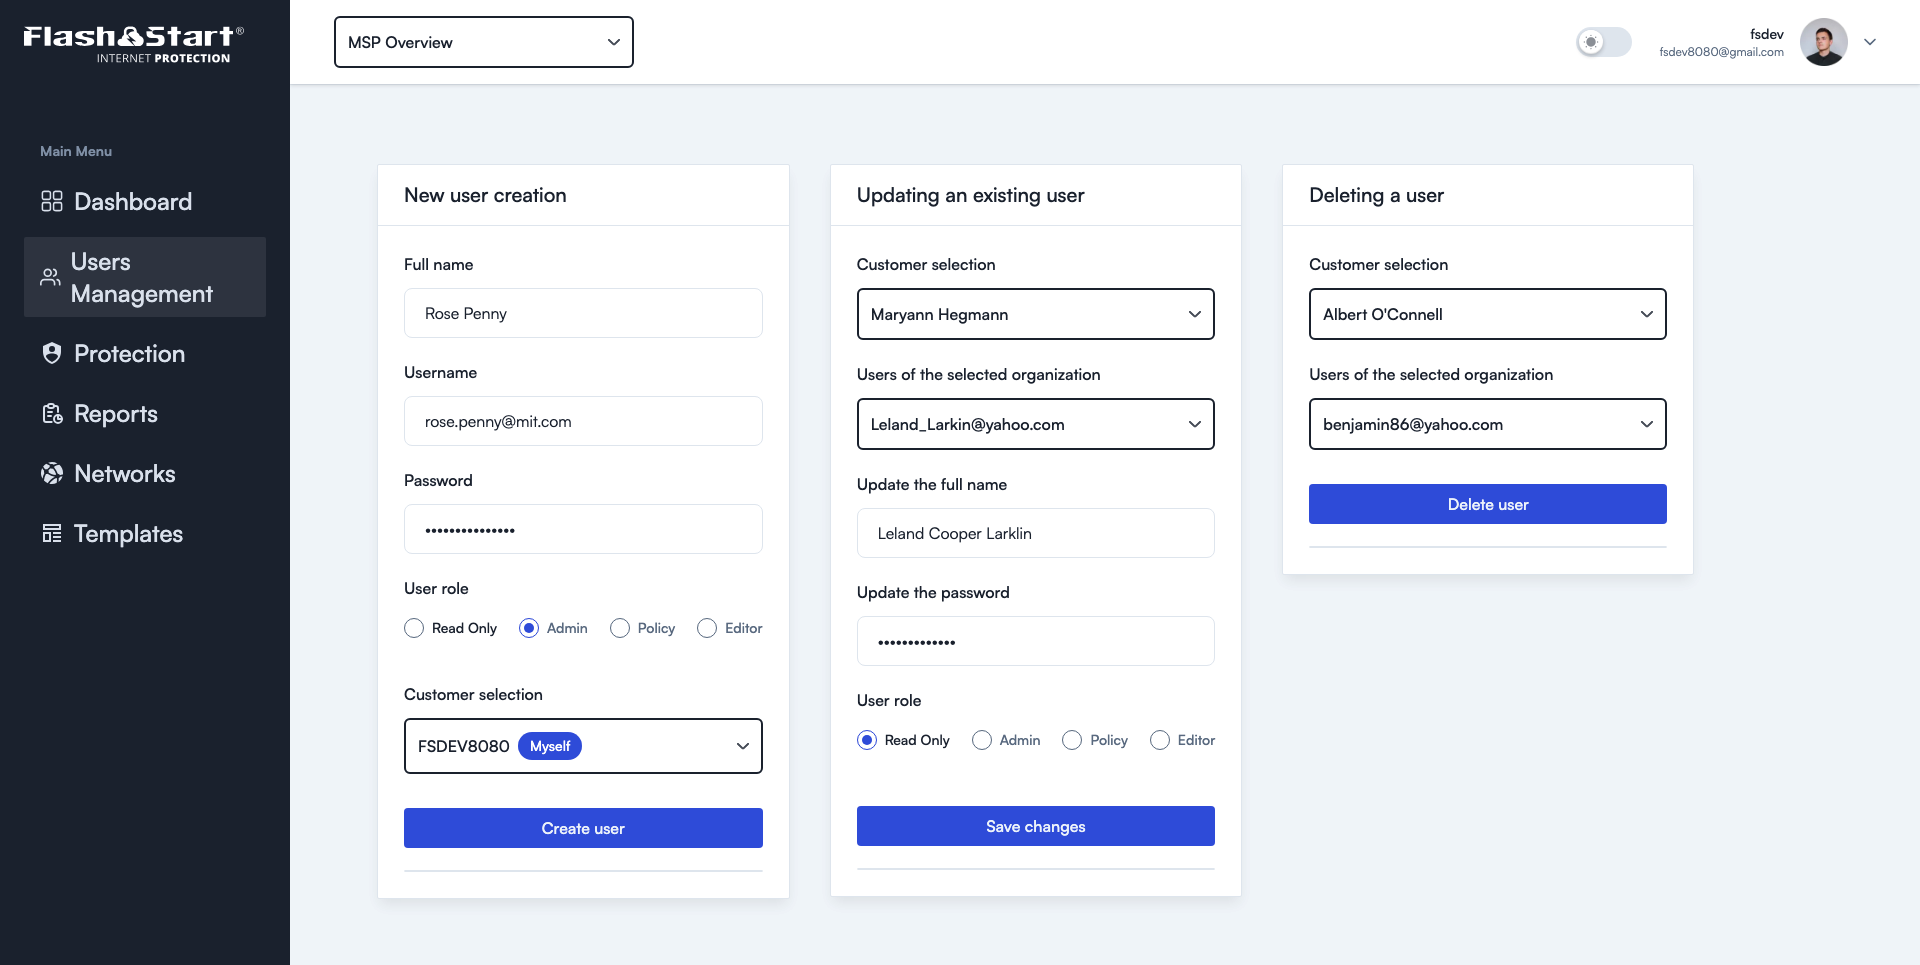
\includegraphics[width=1\textwidth]{figures/new-user-panel.png}
  \caption{Schermata del nuovo sistema per la gestione degli utenti.}
  \label{fig:user-management}
\end{figure}

\subsubsection{Supporto multilingua}
Un ulteriore requisito già soddisfatto è il supporto multilingua. Il frontend del nuovo sistema, infatti, possiede già il supporto completo alle lingue italiano e inglese. Sebbene possa sembrare un dettaglio secondario, questa funzionalità è fondamentale per un prodotto destinato a un mercato internazionale, in cui gli utenti parlano lingue diverse. Inoltre, l’architettura progettata consente di aggiungere nuove lingue in modo semplice, senza necessità di modifiche al codice sorgente, ma solo integrando nuovi file di traduzione.

\subsubsection{Gestione avanzata degli errori}
Un altro elemento progettato e implementato è la gestione avanzata degli errori, che introduce una strategia scalabile e strutturata per il trattamento delle anomalie sia lato backend che frontend.
%
Questa architettura garantisce diversi vantaggi:
\begin{itemize}
  \item \textbf{Robustezza e controllo a tutti i livelli del sistema}: la gestione degli errori è strutturata in modo gerarchico, coprendo dalla validazione degli input nelle API fino ai problemi a livello di database, evitando che errori non gestiti possano propagarsi in modo incontrollato.
  \item \textbf{Standardizzazione e interoperabilità}: gli errori vengono generati in modo schematizzato e dinamico, garantendo una rappresentazione uniforme e facilmente interpretabile da qualsiasi componente del sistema, sia interno che esterno.
  \item \textbf{Compatibilità con il sistema multilingua}: grazie alla struttura modulare degli errori, il frontend può costruire dinamicamente messaggi testuali in più lingue, senza dipendere da stringhe fisse predefinite nel backend.
  \item \textbf{Affidabilità del codice grazie a TypeScript}: il sistema di gestione degli errori sfrutta la tipizzazione statica di TypeScript, garantendo una maggiore sicurezza nella gestione delle eccezioni e facilitando l’individuazione di problemi già in fase di sviluppo.
\end{itemize}

Rispetto al sistema legacy, che gestiva gli errori in modo frammentato e poco strutturato, questa soluzione garantisce una maggiore affidabilità complessiva, riducendo il rischio di comportamenti inattesi e migliorando la manutenibilità del codice. Inoltre, la sua scalabilità consente di adattarlo facilmente a nuove esigenze, rappresentando un elemento chiave per la futura evoluzione del sistema.

\subsection{Elementi solo progettati}
In aggiunta alle funzionalità già realizzate, si evidenzia l’esistenza di alcuni aspetti che, sebbene non ancora sviluppati in maniera operativa, risultano già completamente definiti dal punto di vista progettuale. Nonostante la loro efficacia pratica non sia al momento valutabile, è comunque possibile analizzare il potenziale e il valore aggiunto che tali elementi apporteranno rispetto al sistema legacy.

\subsubsection{Gestione dei profili condivisi}
Uno degli elementi più significativi in questa categoria è l’introduzione dei profili condivisi. Questa novità consente di creare profili di protezione condivisibili tra più organizzazioni all'interno della stessa gerarchia. Essi possono essere visti come template di protezione, utili soprattutto per gli MSP e per i Dealer, che potranno così offrire configurazioni standardizzate e omogenee ai loro clienti.

Un altro vantaggio di questa funzionalità è la semplificazione della gestione della protezione: eventuali modifiche a un profilo condiviso vengono automaticamente propagate a tutte le organizzazioni che lo utilizzano. Questo rappresenta un miglioramento significativo rispetto al vecchio sistema, dove le configurazioni erano gestite separatamente per ogni organizzazione, con difficoltà nella loro manutenzione e uniformità.

L’introduzione dei profili condivisi permette inoltre al sistema di allinearsi con i competitor, alcuni dei quali già dispongono di questa funzionalità. Benché tale caratteristica non sia ancora implementata, la sua progettazione dettagliata consente di avere una chiara roadmap per la sua realizzazione e integrazione futura.

\subsubsection{Riprogettazione del database}
Il design della funzionalità appena descritta rientra in un più ampio processo di rimodellazione del database, che garantisce maggiore scalabilità e coerenza dei dati. Inoltre, la nuova struttura permette l’implementazione di funzionalità avanzate che il vecchio database, per sua natura, non poteva supportare. Questa revisione assicura che il sistema possa evolversi senza le limitazioni strutturali della versione legacy, rendendolo più flessibile, scalabile e adatto alle esigenze future.

Per quanto la riprogettazione del database sia stata completata principalmente a livello di schema concettuale, alcune componenti essenziali risultano già integrate nel sistema. In particolare, le nuove tabelle dedicate alla gestione degli utenti e delle organizzazioni sono già operative e costituiscono la base su cui si fonda il meccanismo di multiutenza. Queste modifiche hanno consentito di superare i vincoli del vecchio modello, che non era stato concepito per supportare una gestione avanzata degli accessi e delle gerarchie organizzative.

L’adozione del nuovo schema dati non solo migliora la struttura e la leggibilità del database, ma assicura anche una maggiore coerenza e manutenibilità, agevolando l’implementazione futura di altre funzionalità chiave. Inoltre, grazie al suo design modulare e scalabile, il database può adattarsi con facilità a nuove esigenze, garantendo flessibilità operativa e una gestione più efficiente dei dati.

\section{Miglioramenti pianificati}
Malgrado il nuovo sistema abbia già introdotto numerosi miglioramenti rispetto alla versione legacy, vi sono ancora diverse aree che non risultano complete, così come altre funzionalità che devono essere introdotte ex novo per garantire un'esperienza conforme alle esigenze operative previste. Tutti i punti trattati in questa sezione rappresentano miglioramenti già pianificati o previsti nella roadmap di sviluppo e verranno implementati nelle fasi successive rispetto a questa tesi.

\subsection{Gestione avanzata dei permessi e autenticazione}
L’attuale implementazione della multiutenza consente la creazione e la gestione di account con differenti ruoli, tuttavia, il controllo degli accessi richiede ulteriori sviluppi. In particolare, è prevista l’integrazione di un sistema \textit{Role-Based Access Control} per la gestione dei ruoli utente, combinato con un livello di autorizzazione che regoli i permessi legati all’organizzazione di appartenenza e alle licenze attive.

Per garantire un sistema di permessi strutturato ed efficace, sarà necessaria un’analisi approfondita per individuare tutte le operazioni da regolamentare e codificare in una tabella del database. Successivamente, il sistema dovrà essere integrato a tutti i livelli della piattaforma, assicurando un controllo uniforme sugli endpoint dell’API e sulle rotte del frontend.

In aggiunta, per migliorare ulteriormente la sicurezza e conformarsi agli standard più recenti, è prevista l’implementazione di un sistema di autenticazione multifattore (MFA). Questo elemento è particolarmente richiesto dai clienti operanti in settori sensibili, dove la protezione degli accessi rappresenta un requisito imprescindibile.

\subsection{Integrazione della brand identity nel frontend}
Attualmente, il frontend del sistema è stato sviluppato con un focus sulle funzionalità, senza un’integrazione effettiva della nuova identità visiva dell'azienda. Nelle fasi successive, è già previsto il coinvolgimento del designer responsabile del rinnovamento dell'immagine aziendale, garantendo così un'interfaccia armonizzata con il design system dell'organizzazione. Sebbene questo aspetto non incida direttamente sulle funzionalità, riveste un ruolo cruciale per l’accettazione del prodotto da parte degli utenti finali, che devono percepirlo come un sistema moderno, affidabile e in linea con l’identità del brand.

\subsection{Implementazione della nuova struttura del database}
Come è già stato evidenziato, la riorganizzazione del database risulta già delineata sotto il profilo concettuale e, attualmente, è stata resa operativa soltanto la componente relativa alla gestione della multiutenza. Per le restanti sezioni, invece, è in corso la traduzione in un database di test.

Un elemento cruciale nella roadmap è la definizione di un processo di migrazione dei dati dal sistema legacy alla nuova base dati. Tale passaggio consentirà di validare fin da subito la coerenza e l’integrità delle nuove tabelle, garantendo al contempo la prosecuzione dello sviluppo sulla versione migliorata del database.

\subsection{Aumento della copertura dei test}
Attualmente, l’infrastruttura di testing del frontend è stata predisposta e resa operativa, ma non dispone ancora di specifiche definite per garantire una copertura adeguata. Tuttavia, la \textit{coverage} al 100\% del codice sorgente rappresenta un requisito fondamentale per garantire la stabilità e l’affidabilità del sistema, in quanto contribuisce a individuare e correggere eventuali anomalie prima del rilascio in produzione.
%
Per soddisfare questo requisito è necessario incrementare la copertura dei test automatizzati, con particolare attenzione ai componenti critici dell’interfaccia utente. Questo aspetto è già stato pianificato e verrà affrontato nelle prossime iterazioni dello sviluppo, al fine di consolidare la qualità del software e ridurre il rischio di regressioni.

\subsection{Implementazione delle funzionalità chiave}
Oltre ai miglioramenti tecnici e architetturali già discussi, il completamento della prima release del sistema richiede l’integrazione di alcune macrofunzionalità fondamentali per garantirne la piena operatività. In particolare, il sistema dovrà includere:
\begin{itemize}
  \item \textbf{Gestione della protezione}: interfacce e strumenti dedicati alla configurazione delle policy di filtraggio e sicurezza, con un'efficace integrazione dei profili condivisi.
  \item \textbf{Generazione e visualizzazione avanzata dei report}: estensione del modulo di reporting per offrire un’analisi più dettagliata rispetto ai dati attualmente disponibili nella dashboard panoramica, così come la possibilità di esportare i report in formati standard.
  \item \textbf{Analisi del traffico in tempo reale}: strumenti per il monitoraggio live delle richieste DNS, utili per una gestione più dinamica della sicurezza di rete. Dovrà essere inclusa una funzione di ricerca avanzata per filtrare e analizzare i dati in tempo reale.
  \item \textbf{Gestione degli Endpoint remoti}: integrazione del sistema con i dispositivi mobili dotati di \textit{ClientShield}, per consentirne la configurazione e il monitoraggio da parte dei gestori del filtro.
\end{itemize}

Il nuovo sistema è destinato a sostituire integralmente il precedente, ragion per cui dovrà integrare fin dalla prima release tutte le macrofunzionalità della versione legacy, garantendo continuità nell’erogazione dei servizi e nella gestione della protezione e del traffico DNS. L’implementazione di tali moduli, dunque, non costituisce un semplice avanzamento, bensì un requisito imprescindibile per assicurare una transizione senza compromessi tra il vecchio e il nuovo sistema.

\subsection{Scrittura della documentazione}
Un aspetto fondamentale per garantire la manutenibilità e l’adozione efficace del nuovo sistema è la creazione di una documentazione completa e strutturata. Questo processo coinvolge tre aree principali: la documentazione del codice, la formalizzazione delle API e la stesura di un manuale utente.

Per quanto riguarda il codice sorgente, è essenziale integrare commenti dettagliati nelle parti più rilevanti e articolate, al fine di agevolare la comprensione della codebase da parte di nuovi sviluppatori. La documentazione interna sarà redatta esclusivamente in inglese, seguendo le best practices per i progetti software con una possibile espansione internazionale.

Parallelamente, sarà necessario predisporre una documentazione formale delle API, che descriva in modo chiaro gli endpoint disponibili, i parametri accettati e i formati di risposta previsti. Questa documentazione sarà tradotta nelle principali lingue per garantire un facile accesso agli sviluppatori esterni e ai partner tecnologici.

Infine, la redazione di un manuale utente sarà essenziale per facilitare l’adozione del nuovo sistema sia da parte dei nuovi utenti sia di coloro che effettuano la transizione dal pannello legacy. Il manuale dovrà includere istruzioni dettagliate sulle funzionalità disponibili e sarà tradotto nelle principali lingue, garantendo un supporto chiaro e accessibile a un’utenza internazionale.

L’implementazione di un processo di documentazione strutturato contribuirà significativamente a migliorare l’esperienza degli sviluppatori e degli utenti, garantendo una maggiore efficienza nella gestione del sistema e una più rapida curva di apprendimento.


%----------------------------------------------------------------------------------------
% BIBLIOGRAPHY
%----------------------------------------------------------------------------------------

\backmatter

\nocite{*} % Remove this as soon as you have the first citation

\bibliographystyle{alpha}
\bibliography{bibliography}

% \begin{acknowledgements} % this is optional
% Optional. Max 1 page.
% \end{acknowledgements}

\end{document}
